\documentclass[12pt]{ociamthesis}  % default square logo 
%\documentclass[12pt,beltcrest]{ociamthesis} % use old belt crest logo
%\documentclass[12pt,shieldcrest]{ociamthesis} % use older shield crest logo

% pakiety ze strony pjatk
\pagenumbering{gobble}
\usepackage[T1]{fontenc}
\usepackage{lmodern,cmap}
\usepackage[none]{hyphenat}


%load any additional packages
\usepackage{amssymb}
\usepackage[utf8]{inputenc}
\usepackage{polski}
\usepackage[polish]{babel}

\usepackage{hyperref} % enables using hyperlinks in captions
\usepackage{float} % allows using option [H] in the positioning of figures
\usepackage{xcolor} % allows defining own colors according to schema \definecolor{myOrange}{rgb}{1, 0.5, 0}

\usepackage{chronosys} % to make a timeline

\definecolor{TODO}{rgb}{1, 0.5, 0}
\definecolor{darkerBlue}{rgb}{0.01 ,0.2, 0.55}
\definecolor{babyblueeyes}{rgb}{0.63, 0.79, 0.95}
\usepackage{hyperref}

\usepackage{pifont} % special characters \ding{number}, np. \ding{70}

\usepackage{listings} % for adding code snippets with labels and captions that can be referenced later
\renewcommand\lstlistingname{Listing}
\renewcommand\lstlistlistingname{Spis listingów}
\def\lstlistingautorefname{Listing. }

\definecolor{codegreen}{rgb}{0,0.6,0}
\definecolor{codeMygreen}{rgb}{0,0.99,0.78}
\definecolor{codegray}{rgb}{0.5,0.5,0.5}
\definecolor{codepurple}{rgb}{0.58,0,0.82}
\definecolor{codeLightBlue}{rgb}{0,0.48,1}
\definecolor{codeyellow}{rgb}{0.67,0.67,0.0}
\definecolor{backcolour}{rgb}{0.95,0.95,0.92}
\definecolor{backcolourWhite}{rgb}{1,1,1.}

\lstdefinestyle{mystyle}{
	language=Python,
	backgroundcolor=\color{backcolour},   
	%backgroundcolor=\color{backcolourWhite},   
	commentstyle=\color{codegreen},
	keywordstyle=\color{codeLightBlue},
	emph={testfunc,print,src},
	emphstyle=\color{codeyellow},
	numberstyle=\tiny\color{codegray},
	stringstyle=\color{magenta},
	basicstyle=\footnotesize,
	breakatwhitespace=false,         
	breaklines=true,                 
	captionpos=t,                    
	keepspaces=true,                 
	numbers=left,                    
	numbersep=5pt,                  
	showspaces=false,                
	showstringspaces=false,
	showtabs=false,                  
	tabsize=2
}

\lstset{style=mystyle}

\usepackage{fancyvrb} % adding indentation to Verbatim (with capital letter)  cells
\usepackage{rotating}

%input macros (i.e. write your own macros file called mymacros.tex 
%and uncomment the next line)
%\include{mymacros}

%\title{Codimension-Two\\[1ex]     %your thesis title,
%        Free Boundary Problems}   %note \\[1ex] is a line break in the title
%
%\author{Keith Gillow}             %your name
%\college{St Catherine's College}  %your college
%
%%\renewcommand{\submittedtext}{change the default text here if needed}
%\degree{Doctor of Philosophy}     %the degree
%\degreedate{Trinity 1998}         %the degree date




%end the preamble and start the document
\begin{document}
	
	

%this baselineskip gives sufficient line spacing for an examiner to easily
%markup the thesis with comments
\baselineskip=18pt plus1pt

%set the number of sectioning levels that get number and appear in the contents
\setcounter{secnumdepth}{3}
\setcounter{tocdepth}{3}


%\maketitle                  % create a title page from the preamble info



\begin{center}
	
\includegraphics[width=1\textwidth]{images/logo_pl.jpg}
	
	\vspace*{1.25cm}
	\textbf{Wydział Informatyki}
	
	\vspace*{1.25cm}
	\textbf{Katedra Data Science}
	
	\vspace*{0.25cm}
	Inteligentne Systemy Przetwarzania Danych
	
	\vspace*{1.25cm}
	\begin{center}
	\textbf{	Autorzy:} \\
	\end{center}
\begin{center}
	\begin{tabular}{ c c }
		\textbf{Lidia J. Opuchlik} \qquad & \qquad \textbf{Sandra Rawicz} \\ 
		Nr albumu s16478 \qquad & \qquad Nr albumu s16536 \\  
   
	\end{tabular}
\end{center}
	
	\vspace{1.5cm}
	{\huge Analiza sentymentu w recenzjach filmowych}
	
	\vspace{0.5cm}
	
	{\large Sentiment analysis in film reviews  \par}
	
	
	
\end{center}

\vspace*{1cm}

\begin{center}
{\large \textbf{Praca inżynierska}}
\end{center}

\vspace*{0.2cm}

\begin{flushright}
	
	\begin{minipage}{0.5\textwidth}
%	\textbf{\begin{center}
%				Praca inżynierska
%	\end{center}}
		
		\vspace{0.5cm}
		\textbf{Promotor:} \\
		dr hab. Grzegorz M. Wójcik, prof. PJATK
	\end{minipage}
	
	
\end{flushright}


\begin{center}
	\vspace*{\fill}
	Warszawa, wrzesień 2021
\end{center}
\thispagestyle{empty}




%\include{dedication}        % include a dedication.tex file
%\include{acknowledgements}  % include an acknowledgements.tex file
%\include{abstract}          % include the abstract
\chapter*{Wkład do pracy}
\thispagestyle{empty}

%%%  ------------> obrazek
\begin{figure}[H]
	\centering
	
\includegraphics[width=1\linewidth]{images/podpis-wklad.pdf}
	\label{fig:wklad}
\end{figure}




%
%Wkład do części pisemnej pracy inżynierskiej był następujący:
%
%\bigskip
%\noindent Cele i streszczenie --- Sandra Rawicz \\
%Rozdział 1 --- Lidia J. Opuchlik \\
%Rozdział 2 --- Sandra Rawicz \\
%Rozdział 3 --- Lidia J. Opuchlik i Sandra Rawicz (po równo) \\
%Rozdział 4 --- Lidia J. Opuchlik \\
%
%
%\bigskip
%\noindent Opracowanie koncepcji oraz modelowanie było wykonywane w równym stopniu przez Lidię J. Opuchlik i Sandrę Rawicz.
%
%\bigskip\bigskip\bigskip
%
%\begin{tabular}{p{7cm} p{5cm}}
%
%	 & 
%	 	Podpis promotora
%	 \\
%		& \\
%		& \\
%     & .............................................................. \\
%
%\end{tabular}
\begin{romanpages}          % start roman page numbering
\tableofcontents            % generate and include a table of contents

\listoffigures              % generate and include a list of figures
\addcontentsline{toc}{section}{Spis rysunków}
\listoftables      % generate and include a list of tables
\addcontentsline{toc}{section}{Spis tablic}
\lstlistoflistings
\addcontentsline{toc}{section}{Spis listingów}
\end{romanpages}            % end roman page numbering



\addcontentsline{toc}{chapter}{Wstęp}
\addcontentsline{toc}{section}{Cel pracy}
\addcontentsline{toc}{section}{Słowa kluczowe}
\addcontentsline{toc}{section}{Streszczenie}

\chapter*{Cel pracy i streszczenie}

\section*{Cel}

Celem ninejszej pracy było stworzenie i zbadanie przydatności klasycznych modeli machine learningowych oraz modeli wykorzystujących sieci neuronowe umożliwiających analizę sentymentu --- klasyfikację czy dana recenzja ma pozytywny czy negatywny wydźwięk --- recenzji filmowych z portalu IMDB (Internet Movie DataBase).

\section*{Streszczenie}

W rozdziale pierwszym niniejszej pracy opisujemy najpierw zagadnienie sztucznej inteligencji --- rys historyczny oraz podstawowe pojęcia. Następnie omawiamy pojedynczą dziedzinę sztucznej inteligencji --- przetwarzanie języka naturalnego. Przybliżamy założenia i metody charakterystyczne dla tej dziedziny. Definiujemy też konstrukcje i metody wykorzystywane w zagadnieniach uczenia maszynowego, do których odwołują się kolejne rozdziały. W szczególności opisujemy problem klasyfikacji binarnej, który rozwiązujemy w ramach niniejszej pracy.

W drugim rozdziale pracy omawiamy wykorzystane przez nas algorytmy: las losowy, maszyna wektorów nośnych, konwolucyjne sieci neuronowe, LSTM, oraz połączenie sieci konwolucyjnej z LSTM. Dla każdego algorytmu opisana jest jego konstrukcja i właściwości, a także szczegóły implementacji wykorzystanej w obrębie pracy.

W trzecim rozdziale pracy przedstawiamy eksperymenty aplikujące poszczególne przedstawione algorytmy do wybranego zbioru danych. Najpierw omawiamy przygotowanie zbioru danych. Następnie dla każdego z algorytmów prezentujemy implementację oraz omawiamy sposób dobrania parametrów modelu. Pokazujemy też estymację przydatności poszczególnych algorytmów za pomocą wybranego zbioru metryk.

W ostatnim rozdziale znajduje się podsumowanie otrzymanych wyników. % cel.tex file
 %now include the files of latex for each of the chapters etc
\chapter{Sztuczna inteligencja}

% http://www.if.pw.edu.pl/~julas/TEXT/pliki/TEXT4.pdf
Koncepcja nowoczesnej sztucznej inteligencji ma swoje korzenie już w pracach klasycznych filozofów, którzy próbowali opisać proces ludzkiego myślenia jako mechaniczną manipulację symbolami.
Wiele wieków później, w latach 40. XX wieku, zwieńczeniem tych prac było wynalezienie programowalnego komputera cyfrowego bazującego na abstrakcyjnym rozumowaniu matematycznym. Urządzenie to i stojące za nim pomysły zainspirowały naukowców do dyskusji na temat możliwości zbudowania „mózgu elektronicznego”.
Badania w tej dziedzinie znacznie przyspieszyły i zróżnicowały się (rozgałęziły) począwszy od lat 50-tych XX wieku, kiedy to Alan Turing --- znany angielski matematyk, kryptolog --- stworzył maszynę Turinga  ---  abstrakcyjny model urządzenia służącego do wykonywania różnych algorytmów. Turing jest uważany za jednego z „ojców” informatyki i sztucznej inteligencji \cite{turing}. W ramach badań nad sztuczną inteligencją zaproponował on wykonanie testu zwanego Testem Turinga, który miał za zadanie sprawdzić czy „wypowiedzi” odpowiednio zaprogramowanej maszyny/algorytmu naśladującego sposób myślenia ludzkiego i posługującego się językiem naturalnym są odróżnialne od wypowiedzi prawdziwego człowieka. Test uznawany jest jako zaliczony, gdy sędzia (człowiek) konwersujący z kilkoma innymi obiektami (kilkoma ludźmi i maszyną) nie jest w stanie stwierdzić, czy w danej chwili rozmawia z człowiekiem, czy z maszyną symulującą człowieka. Od tego ważnego wydarzenia dynamika badań nad przetwarzaniem języka naturalnego (NLP) znacznie przyspieszyła. Ważniejsze kamienie milowe przedstawione są na osi czasu na następnej stronie. Obejmuje ona historię NLP od roku 1950 do czasów obecnych. \\
\noindent W ogólności sztuczna inteligencja jest definiowana jako zdolność systemu do poprawnej interpretacji danych zewnętrznych, uczenia się na podstawie takich danych oraz wykorzystywania tych informacji do osiągania konkretnych celów i zadań wykorzystując elastyczną adaptację \cite{KAPLAN2019}. Sztuczną inteligencję, ze względu na możliwości rozwiązywania przez nią problemów oraz umiejętność dostosowywania się do różnego rodzaju zadań, można podzielić na 3 rodzaje: słabą, ogólną i superinteligencję. \\


%%    http://www.cs.put.poznan.pl/amichalski/wsi/AI1.rgb.pdf


% --------------- TIMELINE ----------------
\startchronology
[
align=left, 
startyear=1950,
stopyear=2021, 
startdate=true, 
stopdate=true, 
dateselevation=-20pt, 
arrow=false,
arrowcolor=black, 
box=true
]

% lata 50-te
\chronoevent[markdepth=-30pt, textwidth=2.5cm, date=false]{1950}{{\small \begin{center}
			\textbf{1950} \\ Test Turinga \cite{turingtesttimeline}
\end{center}}}

% 60-te
\chronoperiode[color=babyblueeyes, startdate=false, stopdate=false]{1956}{1962}{}

\chronoevent[markdepth=20pt, textwidth=3.5cm, date=false]{1959}{{\small \begin{center}
			\textbf{późnie lata 50-te i~wczesne 60-te} \\ sieci semantyczne do tłumaczeń maszynowych \\ \cite{siecisemantyczne}
\end{center}}}
\chronoevent[markdepth=-30pt, textwidth=2.5cm, date=false]{1965}{{\small \begin{center}
			\textbf{1965} \\ ELIZA \\ \cite{eliza}
\end{center}}}

% lata 70-te
\chronoevent[markdepth=20pt, textwidth=2.5cm, date=false]{1975}{{\small \begin{center}
			\textbf{1975} \\ PARRY \\ model paranoika (Colby)
\end{center}}}



% 80-te


\chronoevent[markdepth=-30pt, textwidth=2.5cm, date=false]{1986}{{\small \begin{center}
			\textbf{1986} \\ STUDENT \\ znacznie pojedyńczych słów (Bobrow)
\end{center}}}




\chronoevent[markdepth=20pt, textwidth=2.5cm, date=false]{2011}{{\small \begin{center}
			\textbf{2011}  \\ Watson (IBM) wygrywa w Jeopardy! \\ \cite{jeopardy}
\end{center}}}

\chronoperiode[color=babyblueeyes, startdate=false, stopdate=false]{2011}{2015}{}

\chronoevent[markdepth=-30pt, textwidth=2.5cm, date=false]{2013}{{\small \begin{center}
			\textbf{2011-2014} \\ Apple Siri, asystent Google'a, MS Cortana
\end{center}}}



\stopchronology






%% --------------- TIMELINE ----------------
%\startchronology
%[
%align=left, 
%startyear=1950,
%stopyear=2030, 
%startdate=false, 
%stopdate=false, 
%dateselevation=0pt, 
%arrow=true,
%arrowcolor=babyblueeyes, 
%box=true
%]
%%\chronoperiode[color=darkerBlue, startdate=false, stopdate=false]{1950}{2030}{}
%
%
%% lata 50-te
%\chronoevent[markdepth=-80pt, textwidth=2.5cm, date=false]{1956}{{\small \begin{center}
%			\textbf{1956} \\ Pojęcie sztucznej inteligencji \cite{KAPLAN2019}
%\end{center}}}
%\chronoevent[markdepth=10pt, textwidth=2.5cm, date=false]{1950}{{\small \begin{center}
%			\textbf{1950} \\ Test Turinga \cite{turingtesttimeline}
%\end{center}}}
%
%% 60-te
%\chronoevent[markdepth=60pt, textwidth=3.5cm, date=false]{1958}{{\small \begin{center}
%			\textbf{późnie lata 50-te i~wczesne 60-te} \\ sieci semantyczne do tłumaczeń maszynowych \\ \cite{siecisemantyczne}
%\end{center}}}
%\chronoevent[markdepth=-30pt, textwidth=2.5cm, date=false]{1965}{{\small \begin{center}
%			\textbf{1965} \\ ELIZA \\ \cite{eliza}
%\end{center}}}
%
%% lata 70-te
%\chronoevent[markdepth=10pt, textwidth=2.5cm, date=false]{1974}{{\small \begin{center}
%			\textbf{1974-1980} \\ I. zima AI
%\end{center}}}
%
%\chronoevent[markdepth=-125pt, textwidth=2.5cm, date=false]{1970}{{\small \begin{center}
%			\textbf{1970} \\ propagacja wsteczna
%\end{center}}}
%
%
%% 80-te
%\chronoevent[markdepth=60pt, textwidth=2.5cm, date=false]{1984}{{\small \begin{center}
%			\textbf{1984} \\ Film Terminator
%\end{center}}}
%
%\chronoevent[markdepth=-70pt, textwidth=2.8cm, date=false]{1980}{{\small \begin{center}
%			\textbf{1980-1987} \\ Rozwój AI w~Wlk. Brytanii
%\end{center}}}
%
%\chronoevent[markdepth=-30pt, textwidth=2.5cm, date=false]{1990}{{\small \begin{center}
%			\textbf{1987-1993} \\ II. zima AI
%\end{center}}}
%
%
%
%% lata 90-te
%\chronoevent[markdepth=10pt, textwidth=2.5cm, date=false]{1997}{{\small \begin{center}
%			\textbf{1997} \\ Deep Blue (IBM) pokonuje Garego Kasparova w~szachy
%\end{center}}}
%
%
%
%% 2000-czne
%\chronoevent[markdepth=-100pt, textwidth=2.5cm, date=false]{2001}{{\small \begin{center}
%			\textbf{2001} \\ Film A.I. Steven'a Spielberg'a
%\end{center}}}
%
%
%\chronoevent[markdepth=-30pt, textwidth=1.5cm, date=false]{2009}{{\small \begin{center}
%			\textbf{2010} \\ Kinnect XBOX (CV)
%\end{center}}}
%
%
%
%
%
%\chronoevent[markdepth=90pt, textwidth=2.5cm, date=false]{2019}{{\small \begin{center}
%			\textbf{2015} \\ AlphaGo pokonuje mistrza w Go
%\end{center}}}
%
%
%\chronoevent[markdepth=10pt, textwidth=2.3cm, date=false]{2011}{{\small \begin{center}
%			\textbf{2011}  \\ Watson (IBM) wygrywa w Jeopardy
%\end{center}}}
%
%\chronoevent[markdepth=-100pt, textwidth=2.5cm, date=false]{2014}{{\small \begin{center}
%			\textbf{2011-2014} \\ Apple Siri, asystent Google'a, MS Cortana
%\end{center}}}
%
%\chronoevent[markdepth=-30pt, textwidth=2.2cm, date=false]{2021}{{\small \begin{center}
%			\textbf{2017} \\ konferencja o etyce w AI
%\end{center}}}
%
%
%\chronoevent[markdepth=10pt, textwidth=2cm, date=false]{2026}{{\small \begin{center}
%			\textbf{2020}  \\  GPT-3 (OpenAI)
%\end{center}}}
%
%
%\stopchronology




%
%
%\textcolor{TODO}{Potem napisać jak przez lata rozwijała się sztuczna inteligencja - jakiś krótki rys historyczny i kiedy tak naprawdę zaczął się dynamiczny rozwój - coraz mocniejsze komputery, coraz tańsze przetwarzanie, zasoby do przechowywania itd. Jak obecnie dzieli się sztuczną inteligencję (general, super, itd. - 3 rodzaje). Jakie są wady i jakie potencjalne zagrożenia mogą być z nią związane. Jakie są zalety AI i technologii powiązanych. Co można wyciągnąć i w jaki sposób wykorzystuje się dane - jakie sektory, po co, jakie korzyści biznesowe i niebiznesowe za tym idą itd. Analiza, wizualizacja - jak i po co? Rodzaje technologii - ML, NN, CV, NLP itd. i do czego są wykorzystywane. TO CO PONIŻEJ WRZUCIĆ JAK JUŻ BĘDĘ PRÓBOWAŁA NAWIĄZAĆ DO NLP. Dobór techniki opiera się na tym, z jakimi danymi mamy do czynienia. Napisać też o danych generowanych z różnych urządzeń pomiarowych i czujników, smart homes, zegarki, rózne pulsomierze i inne pierdoły (wspomnieć).} \\




\bigskip

%   http://www.cs.put.poznan.pl/amichalski/wsi/AI1.rgb.pdf
\noindent Głównymi obszarami zastosowań sztucznej inteligencji są:
\begin{itemize}
\item uczenie maszynowe (automatyczne),
\item rozpoznawanie i przetwarzanie obrazów --- diagnostyka medyczna, tworzenie gier, śledzenie, tworzenie sztuki,
\item \textbf{przetwarzanie języka naturalnego (NLP)},
\item robotyka i planowanie działań,
\item tworzenie systemów eksperckich.
\end{itemize}

%%%  ------------> obrazek
%\begin{figure}[H]
%	\centering
%	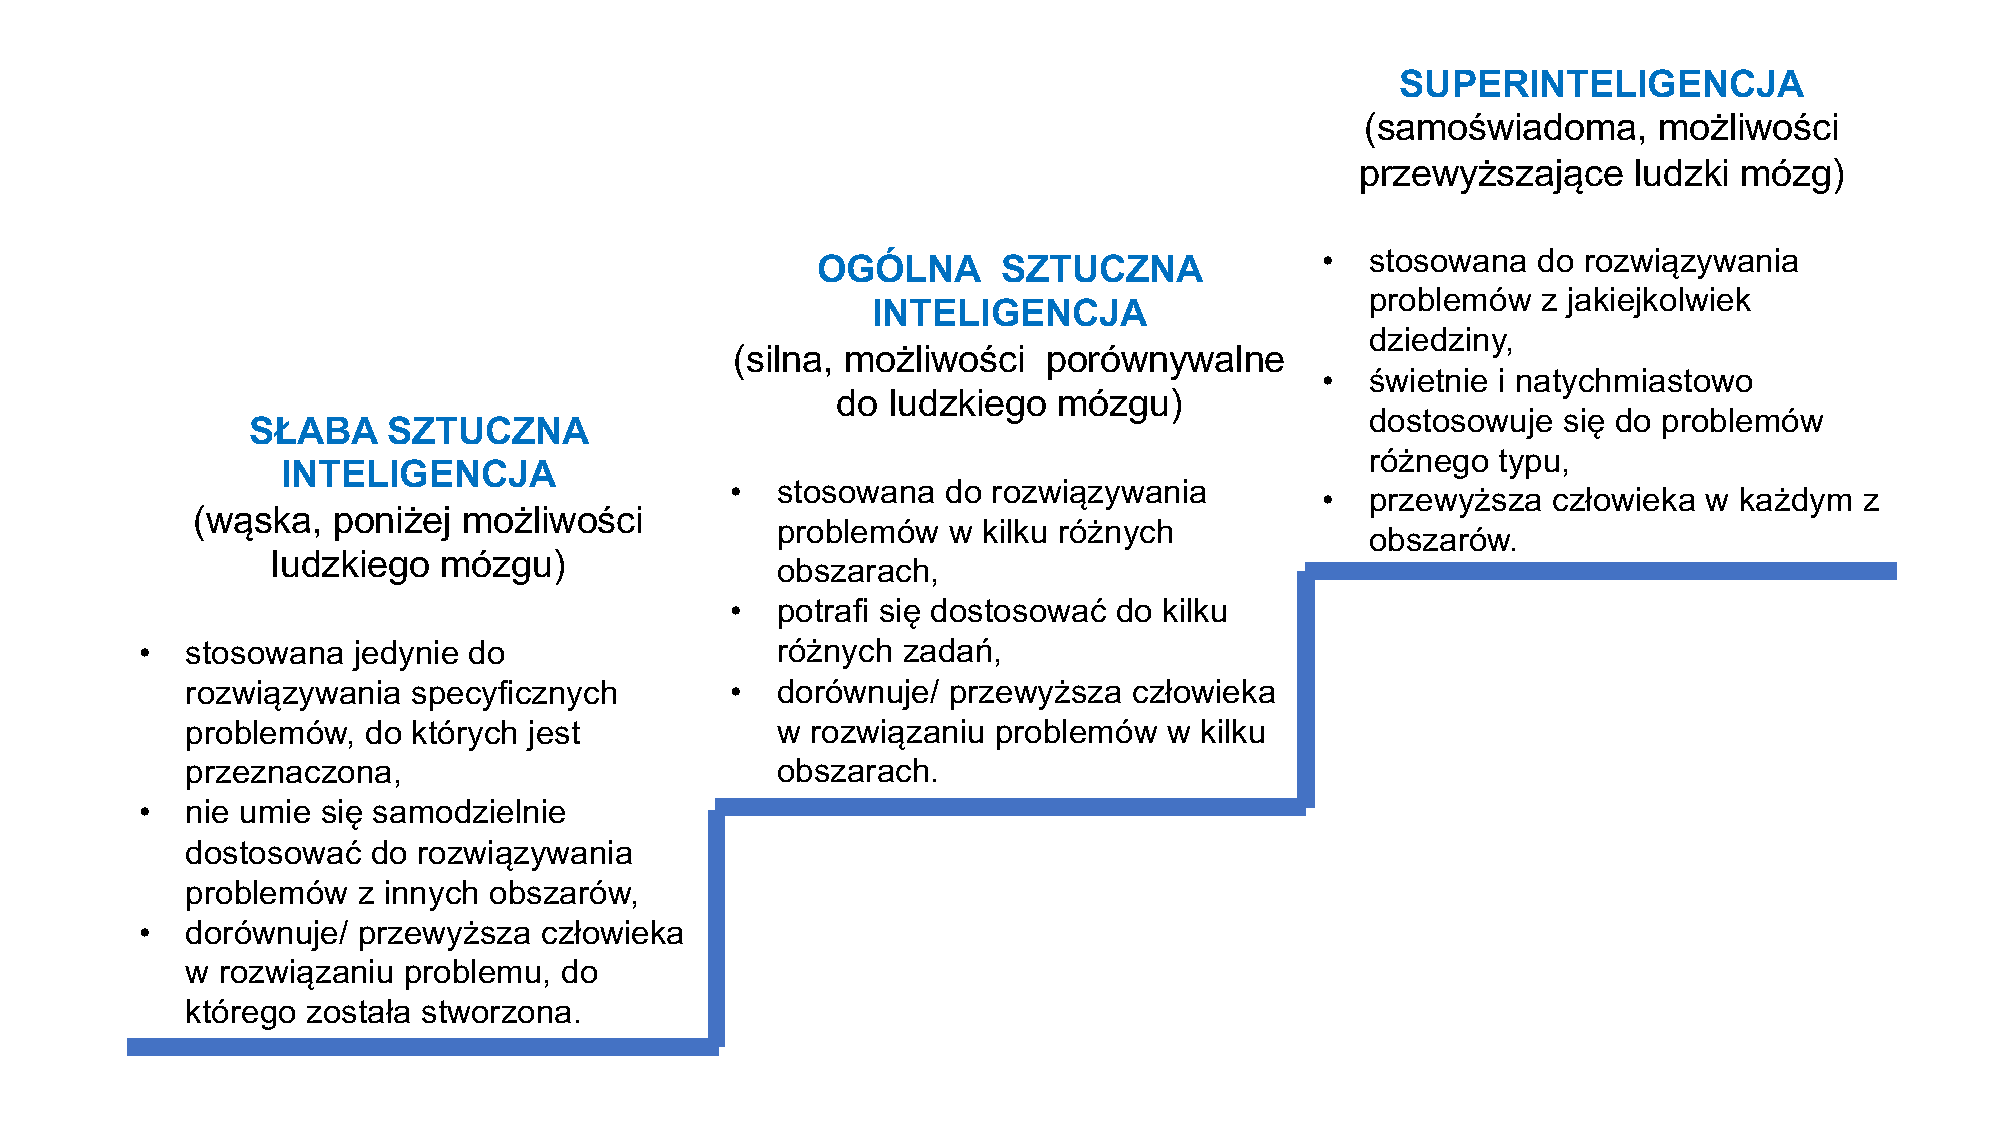
\includegraphics[width=0.95\linewidth]{images/chapter1/weak-general-super-intelligence.pdf}
%	\caption{Rodzaje i możliwości współczesnej sztucznej inteligencji.}
%	\label{fig:narrow-general-super}
%\end{figure}

\bigskip

\noindent Obecnie świat napędzany jest nieustannie rosnącą ilością generowanych danych.  W 2020 roku zostało wygenerowanych, prztworzonych, skopiowanych lub pobranych ponad 64 zettabajy danych. Jeden zettabajt danych, to 10$^{21}$ bajtów. Odnosząc się do danych podawanych przez platformę \copyright~Statista, prognozowana ilość danych ma się mniej więcej potroić do końca 2025 roku \cite{Statista}. Ze względu na tą ogromną ilość ważne jest aby stworzyć efektywne systemy umożliwiające jej wykorzstywanie.


%%%  ------------> obrazek z podpisem hyperlinkiem
%\begin{figure}[H]
%	\centering
%	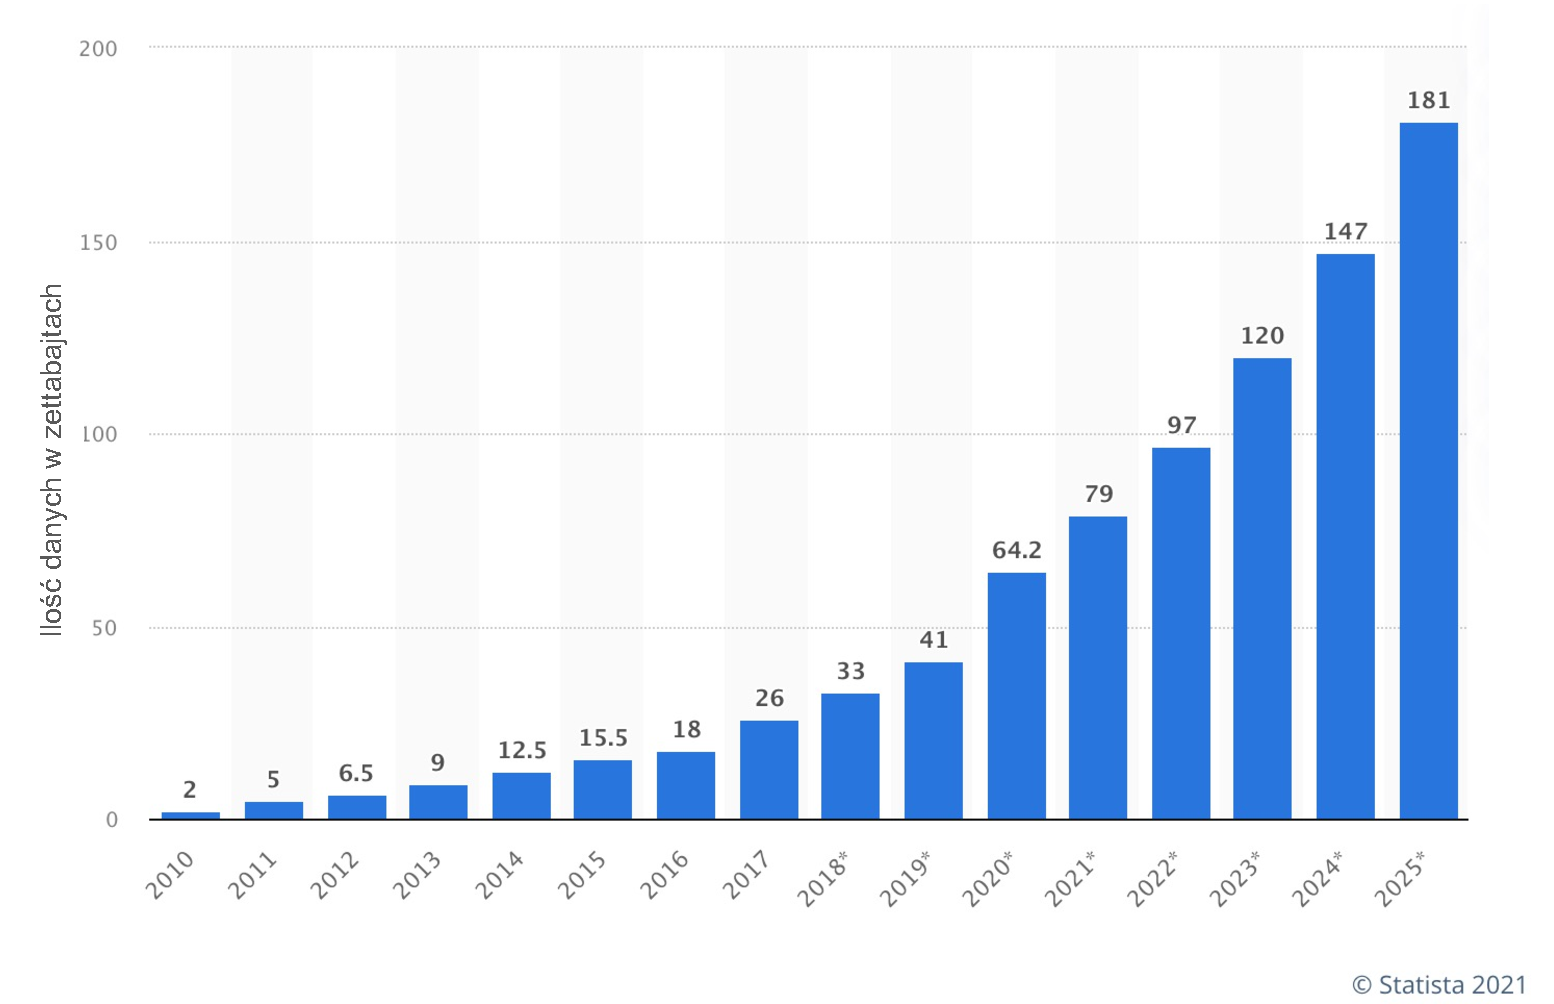
\includegraphics[width=0.95\linewidth]{images/chapter1/data-volume.pdf}
%	\caption{\href{https://www.statista.com/statistics/871513/worldwide-data-created/}{Ilość danych przetwarzanych rocznie w latach 2010 -- 2025.}}
%	\label{fig:data-volume}
%\end{figure}


% z prezentacji

\noindent Wg różnych źródeł około 80\% danych generowanych w obecnych czasach występuje w formie nieustrukturyzowanej, np. jako posty na Facebooku, tweety, opinie, recenzje wystawiane przez użytkowników na portalach internetowych, nagrania audio, wiadomości z Messengera czy Whatsappa oraz dane zbierane przez asystentów głosowych typu Alexa, Siri Cortana itd.
Do danych nieustrukturyzowanych zaliczamy też filmy oraz zdjęcia i wszelką grafikę.
Jednak ze względu na potrzeby tej pracy, skupimy się na danych tekstowych. \\

\noindent Dane nieustrukturyzowane niosą ze sobą mnóstwo użytecznych informacji. Jednak ze względu na nieodłączną złożoność ich przetwarzania i analizowania, praca z nimi stanowi wyzwanie, gdyż dane te trzeba najpierw skrupulatnie wydobyć z surowych zbiorów (nieobrobionych danych źródłowych) lub różnego rodzaju rejestratorów. Jednakże uważamy, że warto poświęcić na to czas, gdyż z biznesowego punktu widzenia nieustrukturyzowane dane stanowią potencjalną kopalnią złota.

\noindent Dla porównania, dane ustrukturyzowane czyli takie, które posiadają konkretną ściśle zdefiniowaną formę stanowią jedynie około 20\% wszystkich generowanych danych, a więc zdecydowaną mniejszość. Jest to kolejny powód, dla którego warto sięgać też po dane nieustrukturyzowane, gdyż korzystanie tylko z tych ustrukturyzowanych danych powoduje, że dużo wartości umyka.
Oba rodzaje wspomnianych danych wykazują istotne różnice. Poniżej wymienione są te najważniejsze.

\begin{table} [H]
	\caption{Porównanie danych ustrukturyzowanych i nieustrukturyzowanych.}
\begin{center}
	\begin{tabular}{ |p{7cm}|p{7cm}|  }
		\hline
		\begin{center}
			Dane ustrukturyzowane 
		\end{center}& \begin{center}
		Dane nieustrukturyzowane
	\end{center} \\  
		\hline
		\ding{70} o jasno zdefiniowanych typach, które można przeszukiwać wg określonych kryteriów & \ding{70} zwykle przechowywane w ich natywnym formacie \\ 
		\ding{70} najczęściej ilościowe & \ding{70} najczęściej jakościowe \\ 
		\ding{70} często przechowywane w hurtowniach danych & \ding{70} często przechowywane w jeziorach danych \\ 
		\ding{70} można je łatwo przeszukiwać i analizować & \ding{70} wymagają więcej pracy --- wstępnej obróbki --- do wydobycia i zrozumienia informacji, które niosą \\ 
		 \ding{70} istnieją we wstępnie zdefiniowanych formatach & \ding{70} występują w różnych formatach \\  
		\hline
	\end{tabular}
\end{center}
\end{table}

\noindent Ze względu na cel niniejszej pracy, skupimy się na możliwościach przetwarzania i analizowania danych w postaci tekstu pisanego (recenzji filmów). Będziemy opierać się na koncepcji przetwarzania języka naturalnego.


\section{Przetwarzanie języka naturalnego}

Dane nie posiadające zdefiniowanej struktury --– w szczególności te tekstowe i głosowe można analizować przy pomocy przetwarzania języka naturalnego.
Wg Wikipedii: przetwarzanie języka naturalnego (\textit{Natural Language Processing}, NLP) to interdyscyplinarna dziedzina, łącząca zagadnienia sztucznej inteligencji i językoznawstwa, zajmująca się automatyzacją języka naturalnego przez komputer, w tym analizą, rozumieniem, tłumaczeniem i generowaniem języka naturalnego \cite{wikipediaNLP}. 
%Systemy rozumiejące język naturalny przekształcają próbki języka naturalnego na bardziej formalne symbole, łatwiejsze do przetworzenia dla programów komputerowych, natomiast systemy generujące język naturalny przekształcają informacje na język łatwy do odczytania i zrozumienia przez człowieka.
%Często rozumienie i generowanie języka idą ze sobą w parze.


\subsection{Do czego wykorzystywane jest NLP?
}
Na pierwszy rzut oka można tego nie zauważyć, ale przetwarzanie języka naturalnego towarzyszy nam w wielu aspektach codziennego życia, i właściwie można stwierdzić, że bez jego obecności trudno byłoby nam funkcjonować.
\\

\noindent Przetwarzanie języka naturalnego wykorzystywane jest:
\begin{enumerate}
\item Do analizy sentymentu --- a poprzez poznawanie opinii użytkowników/klientów --- dalej wykorzystywane jest np. w celu tworzenia spersonalizowanych rekomendacji i reklam, ogłoszeń. Może się to odbywać na podstawie analizy przeprowadzanych ankiet, wypełnianych formularzy, czy po prostu opinii i recenzji pisanych przez użytkowników Internetu,
\item Do automatyzacji różnych procesów:
	\begin{itemize}
	\item kontaktów z klientami --- doradztwo chatbotowe czy ekstrakcja i analiza informacji z nagrań reklamacji itp.,
	\item biurowych --- wyciąganie danych z faktur, dokumentów,
	\item HR-owych ---  do usprawniania procesów rekrutacyjnych, np. analiza i wyciąganie pożądanych informacji z CV czy z portali społecznościowych. Przesłane przez aplikanta CV może nawet nie dojść do żywego rekrutera, bo zostanie już odrzucone na etapie wstępnym w związku z tym, że nie będzie posiadało pewnych elementów czy pożądanych informacji,
	\end{itemize}
\item W urządzeniach Smart Home, np. asystenci głosowi tacy jak Siri, Alexa, Cortana, Google Assistant bazują na rozpoznawaniu i przetwarzaniu mowy, 
\item Do tłumaczenia w czasie rzeczywistym (machine translation), np. google translate,
\item Do sprawdzania pisowni, stylistyki, słownictwa (synonimy), np. Grammarly,
\item W programowaniu --- wszystkie narzędzia intellisense oparte są o NLP, np. Kite,
\item Do wyszukiwania po słowach kluczowych (np. google search zwraca bardzo trafne wyniki wyszukiwania).
\end{enumerate}

\bigskip
\bigskip

\noindent Przetwarzanie języka naturalnego można podzielić na dwie główne gałęzie:
\begin{enumerate}
	\item Rozumienie języka naturalnego,
	\item Tworzenie języka naturalnego.
\end{enumerate}

\bigskip

\noindent Gałąź pierwsza obejmuje wydobywanie informacji z tekstu (\textit{text mining}) i analizę testu (\textit{text analytics}) \cite{wikipediaTM}. Na analizę składają się:
mapowanie surowych danych z tekstów lub nagrań wyrażonych przy pomocy języka naturalnego w ich użyteczną reprezentację, czyli przekształcanie ich w wartościowe informacje, a ponadto nadawanie im odpowiedniej struktury i analiza pewnych cech i wzorców wydobywanych z tych tekstów
oraz analiza aspektów językowych.
Natomiast, gałąź druga polega na wytwarzaniu fraz i zdań oraz dłuższych form  z wewnętrznych reprezentacji mających znaczenie w formie języka naturalnego \cite{wikipediaNLgeneration}.
Gałąź pierwsza jest dużo bardziej pracochłonna i dużo więcej aspektów trzeba zrozumieć żeby wykorzystać to zastosowanie.
Te dwa procesy mogą być ze sobą ściśle powiązane.
\\

\noindent Ogólnym celem NLP jest praca z danymi w języku naturalnym, która umożliwia tworzenie modeli, wyciąganie wniosków w celu produkowania wartości biznesowej.
Jednak żeby korzystać z tego typu nieustrukturyzowanych danych trzeba być zaznajomionym z technikami analizy tekstu i przetwarzania języka naturalnego oraz posiadać do tego spory wachlarz odpowiednich narzędzi.

\subsection{Operacje na danych tekstowych}
Do podstawowych operacji wykonywanych na danych tekstowych należą m. in. tokenizacja, normalizacja, usunięcie niewnoszących do znaczenia tzw. słów-stopów (\textit{stop-words}), stemming, lematyzacja, tagowanie/oznaczanie/rozpoznawanie części mowy (w tym tworzenie N-gramów), rozpoznawanie bytów nazwanych (nazw własnych), parsowanie tekstu --- chunking (parsowanie płytkie)
i parsing (właściwe parsowanie). Należy zaznaczyć, że wykonywanie poszczególnych operacji jest opcjonalne i zależy od zamysłu programisty i użyteczności samej operacji. Najpopularniejszą biblioteką umożliwiającą te operacje jest biblioteka \verb|NLTK| (\textit{Natural Language ToolKi}t). Oprócz funkcjonalności wymienionych wcześniej, biblioteka ta zapewnia również wiele innych bardziej zaawansowanych, nieco rzadziej używanych funkcjonalności.


\subsubsection{Tokenizacja}

Jest to pierwszy etap przetwarzania tekstu polegający na rozbijaniu tekstu na mniejsze struktury --- tzw. tokeny (żetony), np. zdania, wyrażenia, słowa.
Należy tu wyraźnie podkreslić, że znaki przystankowe (kropka, przecinek itd.) też są tokenami.
Przykładowe zdanie --- \textit{Tokenizacja to pierwszy etap w przetwarzaniu języka naturalnego.} --- po wykonaniu tokenizacji zostanie rozbite na następujące tokeny:

%%%  ------------> obrazek
\begin{figure}[H]
	\centering
	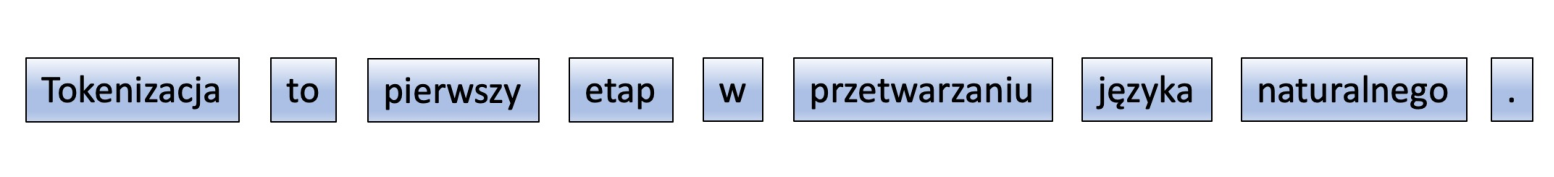
\includegraphics[width=0.95\linewidth]{images/chapter1/tokenizacja.pdf}
	\caption{Zdanie --- Tokenizacja to pierwszy etap w przetwarzaniu języka naturalnego. --- po wykonaniu tokenizacji.}
	\label{fig:tokenizacja}
\end{figure}

\noindent Wygenerowane zostaje tu dziewięć tokenów: \\
$\qquad \rightarrow$ każdy wyraz jest tokenem, \\
$\qquad \rightarrow$  kropka również jest tokenem.


\subsubsection{Normalizacja}
Normalizacja to wykonanie procesów przekształcenia danych tekstowych, które czasami towarzyszą tokenizacji. Normalizacja, inaczej ujednolicenie, może polegać na sprowadzeniu różnych form słów mających podobne (to samo) znaczenie do wspólnej postaci, np. liczebniki znaczące to samo, ale odmienione przez rodzaje --- \textit{jeden}, \textit{jedna}, \textit{jedno} --- należy sprowadzić do postaci \textit{1}, gdyż mają to samo znaczenie. Pominięcie tej procedury skutkowałoby tym, że wyrazy te traktowane by były jako trzy różne słowa mimo, że semantycznie znaczą to samo. Innym zabiegiem normalizacyjnym stosowanym w celu ułatwienia pracy z tekstem jest zamiana wszystkich znaków na znaki tej samej wielkości \cite{normalizacja} --- na wielkie lub małe litery itp. 

\subsubsection{Usuwanie słów-stopów}
Słowa-stopy są to słowa nic nie wnoszące do znaczenia i zrozumienia procesowanych danych (uznawane są za szum). Słowa te (w danym języku) są bardzo powszechnie używane i pojawiają sie właściwie w każdym tekście uniemożliwiając różnicowanie. Wyeliminowanie zbioru tych słów pozwala skupić się na wartościowych treściach (kluczowych słowach umożliwiających skuteczną analizę) \cite{stopwords}. \\
Do słów-stopów zalicza się rodzajniki, spójniki, przyimki itp. Najczęściej są to słowa o najwyższej częstotliwości występowania w tekście. Usuwanie można robić na podstawie dostępnych baz predefiniowanych dla danego języka lub tworzyć własne listy słów-stopów.
Często tworzy się dedykowane listy słów-stopów w zależności od domeny, w której osadzony jest dany tekst. Np., żeby usprawnić analizę tekstu medycznego można usunąć takie słowa jak dr, pacjent itd., żeby analizować wypowiedzi z Twittera można usunąć hashtagi, czyli słowa zaczynające się na \#, nazwy użytkowników --- zaczynające się znakiem @ itp. W ogólności powinno się usuwać wszystkie słowa i frazy, które mają małą moc dyskryminującą i takie, które prowadzą do nieprawidłowości w otrzymywanych wynikach.

%  https://kavita-ganesan.com/what-are-stop-words/#.YQ0ge1MzaL0

\subsubsection{Inne przekształcenia}
Oprócz usuwania słów-stopów można równeż wykonać przekształcenia dające podobny efekt np.
usuwanie akcentów, znaków specjalnych, aposrtrofów, cyfr, czy czegokolwiek niepotrzebnego lub niewnoszącego do zrozumienia niesionej informacji bazując na odpowiednich wyrażeniach regularnych. Przykładem może być usuwanie tagów \verb|HTML|, np. po pobieraniu surowych danych ze strony internetowej (\textit{webscraping}). Przekształcenia te mogą również dotyczyć modyfikacji posiadanych danych. W języku angielskim popularne jest używanie form skrótowych \textit{y'all, I'd, I'll}. Należy je zamienić na \textit{you all}, \textit{I would} oraz na \textit{I will} itd.


\subsubsection{Tworzenie N-gramów}
Tworzenie N-gramów, np. bigramów, trigramów etc. --- polega na tworzeniu połączeń słów, które mogą występować razem. Najpierw się tokenizuje zdanie do słów, a następnie z powstałych tokenów tworzy się N-gramy.
Często zdarza się, że połączenia słów nabierają nowego, innego znaczenia. \\
Przykład: \\
\textit{Nowy Jork} razem ma inne znaczenie niż oddzielne słowa \textit{Nowy} i \textit{Jork}.

\subsubsection{Stemming}
Stemming
to proces usunięcia ze słowa końcówki fleksyjnej (przedrostka, przyrostka) pozostawiając tylko temat wyrazu (nieodmienny rdzeń). Może być przeprowadzany w celu zmierzenia popularności danego słowa. Różne rodzaje stemmerów --- mniej i bardziej agresywne, np. \verb|PorterStemmer| (łagodny), \verb|LancasterStemmer| (bardziej agresywny).

\noindent Wynikiem stemmingu może być ciąg znaków, który sam w sobie nic nie znaczy, ale jest wspólny dla wszystkich słów znaczących to samo w danym tekście jak też normalnym istniejącym i  funkcjonującym słowem. \\
Np. angielskie słowa: \textit{connection}, \textit{connections}, \textit{connective}, \textit{connected}, \textit{connecting} poddane stemmingowi dadzą ten sam wynik, czyli słowo \textit{connect}.

\subsubsection{Lematyzacja}
Lematyzacja to sprowadzenie słowa do jego podstawowej postaci (bazowej), czyli analiza morfologiczna. Do wykonania tego zadania potrzebny jest słownik lub rozbudowany zestaw reguł.
W przypadku czasownika będzie to bezokolicznik, w przypadku rzeczownika --- mianownik liczby pojedynczej. W odróżnieniu od stemmingu --- forma bazowa powstała po lematyzacji zawsze jest  istniejącym słowem.
Warto tutaj dodać, że lematyzacja jest dużo trudniejsza dla silnie fleksyjnych języków ---  takich, które posiadają dużo końcówek dla różnych osób, liczb, przypadków, jak np. język polski. Jest to dużo łatwiejsze w przypadku języka angielskiego.


\subsubsection{Rozpoznawanie części mowy}
Rozpoznawanie części mowy zwane inaczej tagowaniem gramatycznym --- jest to oznaczanie części mowy (POS --- \textit{Part Of Speech}), czyli rozpoznawanie i etykietowanie czy dane słowo jest rzeczownikiem, czasownikiem, przymiotnikiem, przysłówkiem, liczebnikiem itp. Wykonuje się to albo w oparciu o słownik albo wykorzystując występujące końcówki fleksyjne. Może się zdarzyć, że słowo, w zależności od kontekstu, w którym się znajduje, będzie przynależało do różnego typu części mowy . 
\\

\noindent Poniższy przykład dobrze obrazuje wspomnianą niejednoznaczność: \\
$\rightarrow$ \textit{message me} (jako czasownik)
niesie znaczenie daj mi znać lub powiadom mnie, natomiast \\
$\rightarrow$ \textit{a message}  (jako rzeczownik) oznacza po prostu wiadomość.


\subsubsection{Rozpoznawanie bytów nazwanych}
Kolejna operacja na tekście to rozpoznawanie bytów nazwanych. Jest to nic innego jak identyfikowanie/odnajdywanie nazw własnych, które w odróżnieniu od rzeczowników pospolitych, nie są łatwe do rozpoznania, np. lokalizacje, nazwy budynków, dane personalne, waluty, jednostki itp.


\subsubsection{Parsowanie}
Parsowanie to zbieranie indywidualnych „oczyszczonych” kawałków tekstu i grupowanie ich w większe wyrażenia.
Z grubsza, parsowanie można podzielić na dwa rodzaje: parsowanie płytkie (\textit{shallow-parsing}) oraz parsowanie głębokie (\textit{deep-parsing}).

\paragraph{Parsowanie płytkie}
Parsowanie płytkie, czasami określane terminem kawałkowanie (\textit{chunking}), ma na celu wydobycie istotnej informacji, bez potrzeby wyciągania wszystkich zależności składniowych pomiędzy słowami.
Kawałkowanie bierze na wejściu pojedyncze części mowy i zwraca na wyjściu grupy wyrazów/ wyrażenia (\textit{chunki}).
Istnieje 5 głównych rodzajów wyrażeń (grup/\textit{chunków}):
\begin{itemize}
	\item wyrażenia rzeczownikowe (NP),
	\item wyrażenia czasownikowe (VP),
	\item wyrażenia przymiotnikowe (ADJP),
	\item wyrażenia przysłówkowe (ADVP),
	\item wyrażenia przyimkowe (PP).
\end{itemize}

%%%  ------------> obrazek
\begin{figure}[H]
	\centering
	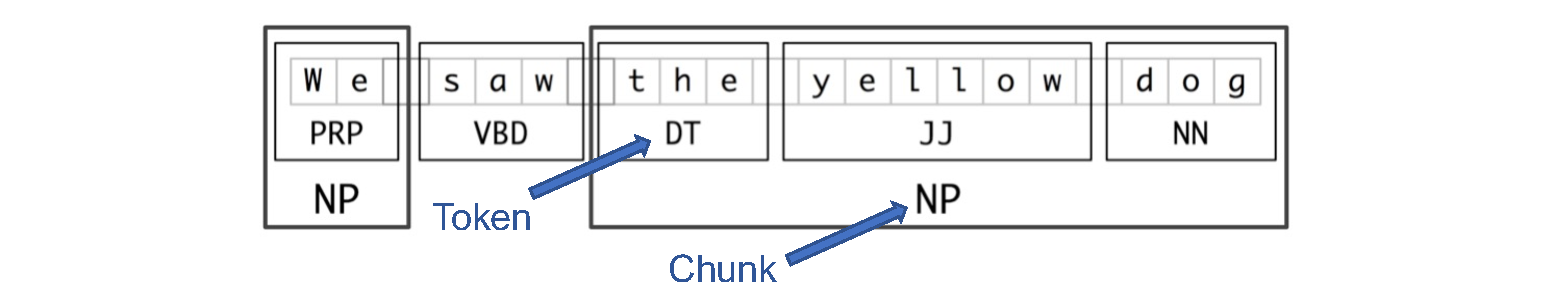
\includegraphics[width=0.95\linewidth]{images/chapter1/shallowParsing.pdf}
	\caption{\href{http://www.nltk.org/book/ch07.html}{Parsowanie płytkie.}}
	\label{fig:shallowParsing}
\end{figure}



\paragraph{Parsowanie głębokie}
Parsowanie głębokie polega na pełnym odtworzeniu drzewa składniowego zdania. 
\\

\noindent Wszystkie wyżej opisane zabiegi stosuje się po to żeby jak najbardziej uprościć budowany model (zmniejszyc jego rozmiary). Jednakże żaden algorytm nie może używać bezpośrednio słów żeby wykoywać modelowanie. Aby budować modele matematyczne, należy przekształcić  słowa w wartości liczbowe (w NLP  w wektory liczb). Gdy dojdzie się do tego punktu, tak naprawdę zabawa się dopiero zaczyna. Można zrobić takie rzeczy, jak wyznaczanie częstotliwości słów w tekście, mierzenie odległości między słowami, wyznaczanie wielu innych przydatnych zależności i parametrów oraz tworzenie modeli klasyfikujących, klasterujących i innych. Istnieje też wiele bibliotek, przy pomocy których można również tworzyć bardzo efektowne wizualizacje.

\section{Podstawy modelowania}
% nazwy bibliotek
%  \verb_sklearn.ensemble.RandomForestClassifier_ 
\subsection{Definicje}
\subsubsection{Uczenie maszynowe}
Uczeniem się systemu jest każda autonomiczna zmiana w systemie zachodząca na podstawie doświadczeń, która prowadzi do poprawy jakości jego działania \cite{cichosz2000}.\\
Uczenie maszynowe to dziedzina nauki dająca komputerom możliwość uczenia się bez konieczności ich jawnego programowania \cite{samuel1959}.  Mówiąc bardziej technicznie uczenie maszynowe polega na tym, że program komputerowy uczy się na podstawie doświadczenia (E) w odniesieniu do jakiegoś zadania (T) i pewnej miary wydajności (P), jeżeli jego wydajność wzrasta wraz z nabywaniem doświadczenia \cite{mitchell}.

\begin{figure}[H]
	\centering
	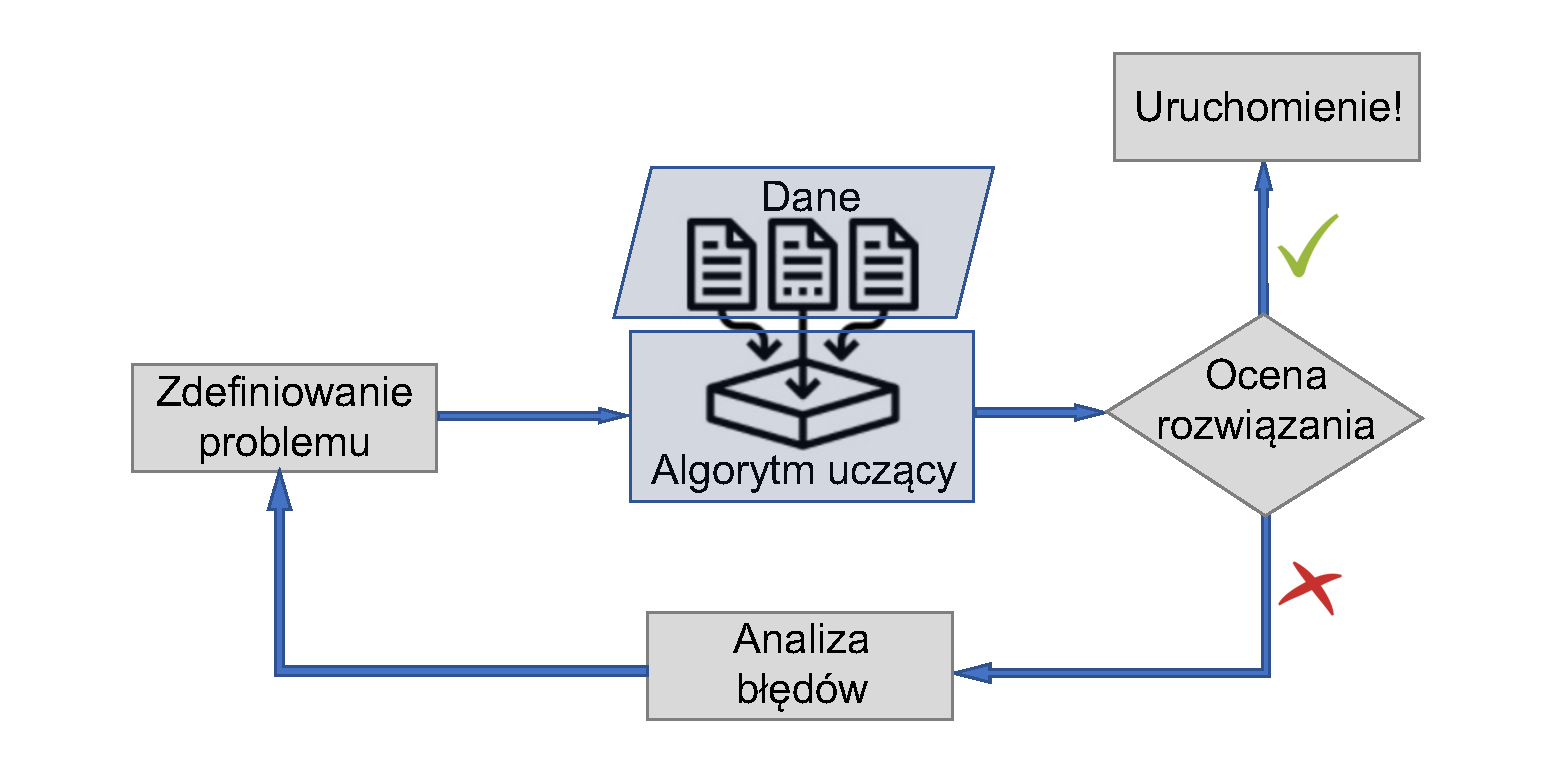
\includegraphics[width=0.75\linewidth]{images/chapter1/machineLearning.pdf }
	\caption{Proces uczenia maszynowego.}
	\label{fig:machine_learning}
\end{figure}


Uczenie maszynowe można podzielić na trzy główne typy:
\begin{enumerate}
	\item Uczenie nadzorowane (\textit{supervised learning}) --- maszyna uczy się generalizować na podstawie oznakowanych danych. W pierwszym etapie nastepuje trenowanie modelu: model jest trenowany na podstawie macierzy cech (\textit{features, atributes}) i odpowiadającym wartościom na wyjściu (\textit{label}). Polega to na dopasowaniu funkcji jak najlepiej odzwierciedlającej dane (generalizującej). Następnie wyznaczony model używa się w predykcji --- na wejściu podaje się macierz z nowymi wartościami cech i wytrenowany model wnioskuje wartość wyjścia (dyskretną --- klasę lub ciągłą --- liczbę) wykorzystując wyuczoną funkcję.
	\item Uczenie nienadzorowane (\textit{unsupervised learning}) --- ma miejsce, gdy informacja trenująca jest niedostępna (brak przynależności do klas wynikowych). De facto używany algorytm sam wyznacza klasy --- znajduje opisy dla tych klas (reguły podziału: jakie klasy są obecne i co je różnicuje) --- i dzieli obserwacje pomiędzy te klasy wg własnego uznania. Proces ten jest często określany mianem grupowania (\textit{clustering}). Należy tu podkreślić, że w zależności od użytego algorytmu, klasy mogą być zdefiniowane w różny sposób --- może istnieć wiele różnych sposobów dzielenia obserwacji na klasy i opisywania każdej klasy, dlatego rodzaj użytego algorytmu ma tu kluczowe znaczenie.
	\item Uczenie wspomagane (\textit{reinforcement learning}).
\end{enumerate}

\subsubsection{Model predykcyjny}
Model predykcyjny opisuje zależności między zmiennymi objaśniającymi (cechami) a zmienną wynikową (targetem) \cite{website}. Umożliwia on, w oparciu o zmienne objaśniające, domniemać jaka jest wartość targetu. Istnieje wiele rodzajów modeli. Przykładami są regresja logistyczna, regresja liniowa, drzewo decyzyjne. \\

\noindent Modele można podzielić ze względu na ich przeznaczenie na:
\begin{itemize}
	\item klasyfikujące --- target dyskretny (np. drzewa decyzyjne, regresja logistyczna),
	\item aproksymujące --- target ciągły (np. regresja liniowa, sieci neuronowe),
	\item asocjujące --- współwystępowanie wartości (np. algorytm A-Priori, sieci asocjacyjne),
	\item segmentujące --- podział na segmenty (np. algorytm k-means, sieci Kohonena).
\end{itemize}

\subsubsection{Klasa}
Klasa --- inaczej target lub zmienna wynikowa lub etykieta --- jest to wartość docelowa wyznaczana przez model predykcyjny, która ma formę dyskretną (nieciągłą).

\subsubsection{Klasyfikacja binarna}
Klasyfikacja binarna --- inaczej regresja logistyczna, to przykład modelu klasyfikacyjnego, w którym na podstawie danych objaśniających nadawane są przynależności do jednej z \textbf{dwóch} możliwych dyskretnych klas wynikowych. Przykładowo na podstawie pewnych określonych charakterystycznych objawów można zakwalifikować pacjenta jako zdrowego lub chorego.

\subsubsection{Algorytm trenujący}
Model może zostać wytrenowany przy pomocy różnych algorytmów trenujących. Algorytmy te mogą różnić się, np. hiperparametrami i ich wartościami oraz dochodzić do wyniku w nieco różny sposób.


\subsubsection{Próbka}
Jest to każdy „element” wykorzystywany do uczenia modelu, tzw. przykład uczący --- pojedyńcza kombinacja cech (atrybutów) wraz z etykietą odpowiadającą tym cechom \cite{geron}. Mówiąc kolokwialnie, jest to jeden wiersz/ rekord/ obserwacja/ obiekt w \verb|Dataframie|.

\subsubsection{Atrybut}
Atrybut --- inaczej cecha (\textit{feature}) --- jest to jeden z aspektów danej próbki. Pojedyńczy atrybut reprezentowany jest jako pojedyńcza kolumna w \verb|Dataframie|. Atrybuty mogą być proste (niepodzielne/ atomowe) lub złożone (można je podzielić na „mniejsze” atrybuty, np. adres zawierający miasto, ulicę, numer, kod pocztowy można rozbić na składowe), kategoryczne lub numeryczne. Atrybuty można również podzielić na niezależne (cechy wykorzystywane do wykonania predykcji) oraz zależne (wyniki predykcji --- tzw. etykiety) \cite{website}.

\subsubsection{Zbiór treningowy}
Zbiór treningowy (\textit{training set}) --- jest to zbiór danych, który używany jest do uczenia się modelu (algorytmu). Na podstawie tych danych model uczy się odpowiednio klasyfikować lub aproksymować wartości wyjścia oraz buduje wszelkie zależności. Inaczej mówiąc, model uczy się przewidywać możliwe wyniki i podejmować decyzje na podstawie przekazanych mu danych \cite{geron}.
\subsubsection{Zbiór testowy}
Zbiór testowy (\textit{testing set}) --- jest to zbiór danych, którego używa się do przetestowania wcześniej wytrenowanego na danych treningowych modelu. Należy podkreslić, że dane zawarte w zbiorze testowym nie mogą być używane wcześniej do nauki modelu (dane, których model nigdy wcześniej nie widział), ponieważ nie będą się wtedy nadawać do obiektywnej oceny działania/skuteczności modelu. Zbioru tego można również użyć w procesie dobierania odpowiedniego zetawu hiperparametrów dla danego modelu \cite{raschka}. \\

\noindent Aby podzielić wyjściowy zbiór danych na treningowy i testowy można użyć popularnej metody \verb|train_test_split| z pakietu \verb|sklearn.model_selection|.


\subsubsection{Hiperparametry}
Zazwyczaj modele w uczeniu maszynowym posiadają parametry. Niektóre mają ich więcej drugie mniej --- w zależności od złożoności danego modelu. Gdy wartość parametru obliczana jest samodzielnie przez algorytm podczas procesu trenowania to parametr taki nazywamy po prostu zwykłym parametrem, natomiast jeżeli wartość parametru zostaje podana przez modelarza, który danego algorytmu używa, to taki specjalny parametr nosi miano hiperparametru \cite{mamczur}. Przykładem hiperparametrów (zewnętrznych parametrów) są, np. głębokość lasu losowego (liczba drzew) czy liczba epok treningowych, natomiast zwykłymi (wewnętrznymi) parametrami mogą być wagi w sieciach neuronowych, czy współczynniki w regresji liniowej.


\subsubsection{Funkcja kosztu (straty)}
Tworzony model, czyli de facto funkcja dopasowywana do danych wejściowych modelu zwana jest powszechnie hipotezą. Dokładność funkcji hipotezy (w stosunku do zbioru uczącego) można zmierzyć za pomocą funkcji kosztu. Przykładem funkcji kosztu może być średni kwadratowy błąd (\textit{mean squared error}). W dużym skrócie, funkcja kosztu zwraca średnią różnicę między wynikami funkcji hipotezy a rzeczywistymi danymi wyjściowymi dla każdego wejścia.
Celem jest minimalizacja tej funkcji kosztu, czyli znalezienie odpowiednich optymalnych parametrów. Im mniejsza wartość funkcji kosztu, tym dokładniejsza jest funkcja hipotezy, czyli lepiej dopasowany jest nasz model \cite{andrewng}.

%\textcolor{TODO}{Dopisać może wzór przykładowej funkcji kosztu z Andrew Ng}

% https://ichi.pro/pl/uczenie-maszynowe-funkcje-kosztow-88976465788030


\subsubsection{Błąd}
Błąd jest to różnica pomiędzy wartością otrzymaną a wartością rzeczywistą (prawdziwą) dla danej obserwacji. Technicznie, błąd można wyznaczać na wiele różnych sposobów. Najczęściej błąd podaje się jako uśrednioną wartość błędów obliczoną dla całego zbioru danych.

\subsubsection{Walidacja --- metryki sukcesu (\textit{model evaluation metrics})}
 Walidacja jest to proces oceny przydatności danego modelu. Do walidacji działania stworzonego modelu stosuje się różne metryki sukcesu. Sa to takie wielkości, które mówią jak dobrze dany model nauczył się generalizować, a co za tym idzie pozwalają nam określić przydatność danego modelu do wykonywania określonego zadania. W problemach klasyfikacyjnych często do oceny używa się macierzy omyłek, która posiada informacje o prawidłowo i nieprawidłowo sklasyfikowanych przykładach w odniesieniu do prawdziwych wartości dla danych przykładów. W oparciu o nią można później obliczyć różne metryki sukcesu. Bardzo popularną metryką jest precyzja (\textit{accuracy}) --- obliczana jako liczba dobrze sklasyfikowanych przykładów do liczby wszystkich przykładów.

\subsubsection{Przeuczenie (\textit{overfitting})}
Przeuczenie (\textit{overfitting}) polega na tym, że model przesadnie dopasowuje się do konkretnych danych --- tych, na podstawie których został zbudowany. Dla tych konkretnych danych zwraca on wyniki obdarzone bardzo małym błędem, natomiast nie umie on dobrze generalizować, a co za tym idzie, jeżeli nakarmimy model nowymi danymi otrzymamy znacznie gorsze wyniki. Przeuczenie następuje, gdy model statystyczny ma zbyt dużo parametrów w stosunku do rozmiaru próby, na podstawie której był konstruowany \cite{overfitting}.

%%%  ------------> obrazek
\begin{figure}[H]
	\centering
	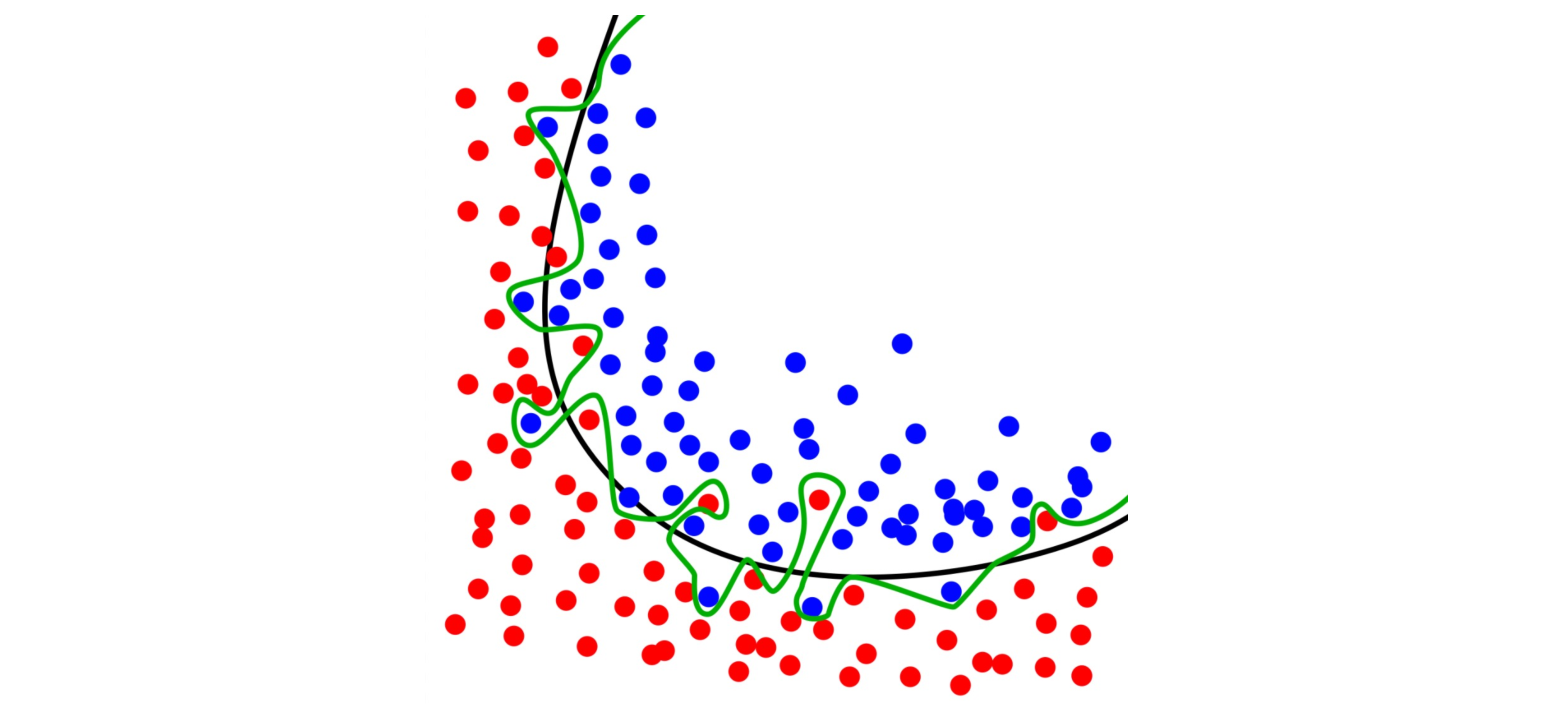
\includegraphics[width=0.95\linewidth]{images/chapter1/overfitting.pdf}
	\caption{\href{https://upload.wikimedia.org/wikipedia/commons/1/19/Overfitting.svg}{Przeuczenie (overfitting).}}
	\label{fig:overfitting}
\end{figure}

\noindent Zielona linia reprezentuje model przesadnie dopasowany (przeuczony), a czarna linia reprezentuje model uregulowany. Chociaż zielona linia najlepiej podąża za danymi treningowymi, jest zbyt zależna od tych danych i prawdopodobnie będzie miała wyższy poziom błędów w przypadku nowych danych w porównaniu z czarną linią. Czarna linia zdecydowanie lepiej generalizuje.



\subsubsection{Wektoryzacja tekstu}
Większość istniejących algorytmów trenujących modele predykcyjne wymaga na wejściu wektorów liczbowych. Istnieje wiele technik pozwalających zamienić tekst na wektor liczb rzeczywistych. Najprostszą techniką jest użycie wektoryzacji zliczeniowej (\textit{Count Vectorization).} Wg dokumentacji \verb|ScikitLearn|, wektoryzacja ta polega na konwersji kolekcji dokumentów tekstowych na macierz zawierającą zliczenia poszczególnych tokenów \cite{countVectorizer}. Mówiąc prościej, polega na zliczaniu słów w danym tekście (korpusie) i w rezultacie umożliwia obliczenie częstości występowania danego słowa w analizowanym tekście. Zaimplementowana jest ona w pakiecie \verb|sklearn.feature_extract-| \verb|ion.text.CountVectorizer|. Rozkład częstości słów można wizualizować przy pomocy wykresów używając metody \verb|FreqDistVisualizer| z pakietu \verb|yellowbrick.text|.\\

%\chapter{Środowisko obliczeniowe}

Wszystkie obliczenia opisane w ramach niniejszej pracy wykonano w środowisku Google Collab na instancji [TODO ile RAMU ile procesora - google nie udostępnia tych danych !!!!!!], za pomocą interaktywnego narzędzia Notebook. Użyto języka Python w wersji 3.6.8 wraz z następującymi bibliotekami:
\begin{itemize}
	\item numpy w wersji 1.19.5 - biblioteka do efektywnych obliczeń naukowych
	\item pandas w wersji 1.1.5 [TODO] - [TODO co to]
	\item … [TODO]
\end{itemize}

\section{Dane}
\subsection{Dane wejściowe}

Wejściowy zbiór danych pochodzi z serwisu \href{https://ai.stanford.edu/~amaas/data/sentiment/}{IMDB (imdb.com)}. Jest to popularny zbiór danych wykorzystywany jako benchmark wielu technik przetwarzania języka naturalnego [TODO odniesienia do publikacji / artykułów gdzie jest wykorzystywany ?]. Składa się z pięćdziesięciu tysięcy recenzji różnych filmów. Każda recenzja jest oznaczona jako pozytywna bądź negatywna. Stosunek recenzji pozytywnych do negatywnych wynosi 1:1. Plik wejściowy ma format CSV z dwiema kolumnami: review - zawiera fragment HTML z tekstem recenzji, oraz sentiment - odpowiednio positive lub negative.
[Opcjonalnie wrzucić screen z kilkoma pierwszymi wierszami]

\subsection{Przygotowanie danych wejściowych}

Zbiór danych wejściowych został wczytany do obiektu typu pandas.Dataframe. Kolumna sentiment została zamieniona na wartości liczbowe - odpowiednio 0-negative oraz 1-positive. Z kolumny reviews, z formatu HTML za pomocą narzędzia BeautifulSoup został wyekstraktowany tekst recenzji. Dane zostały podzielone w sposób losowy na zbiór treningowy oraz testowy w stosunku 4:1. W dalszych krokach, jedynie zbiór treningowy był wykorzystywany do stworzenia modeli predykcyjnych, natomiast zbiór testowy został wykorzystany do ostatecznej walidacji i porównania otrzymanych modeli.
\chapter{Narzędzia i algorytmy}
\label{chapter:2}

W niniejszym rozdziale opisane są wybrane algorytmy służące do klasyfikacji binarnej --- las losowy, maszyna wektorów nośnych, sieci konwolucyjne oraz rekurencyjna sieć LSTM (długoterminowa pamięć krótkoterminowa). Dla każdego algorytmu opisana jest jego konstrukcja i właściwości, a także szczegóły implementacji na potrzeby niniejszej pracy.

\section{Las losowy}
\label{sec:rf}

Las losowy to szeroko wykorzystywana metoda uczenia maszynowego, mogąca posłużyć do rozwiązania problemu klasyfikacji. Polega ona na wytrenowaniu wielu drzew decyzyjnych na losowych podzbiorach danych wejściowych. W celu uzyskania predykcji, sprawdzane są predykcje tak uzyskanych drzew --- predykcja lasu to klasa wybrana przez większość drzew w lesie. Las losowy ma lepsze możliwości dostosowania się do danych wejściowych niż prostsze modele (np. liniowe), ale jest bardziej odporny na przetrenowanie (\textit{overfitting}) niż drzewo decyzyjne.
W tej sekcji opisana jest metoda drzewa decyzyjnego, następnie konstrukcja lasu losowego, potem omówione są kluczowe właściwości lasu losowego, zaś na końcu szczegóły implementacji algorytmu na potrzeby niniejszej pracy.

\subsection{Drzewo decyzyjne}
\label{subsec:dt}

Drzewo decyzyjne to jedna z podstawowych metod wykorzystywana w data miningu dla klasyfikacji \cite{rokach2007data}. Polega ona na zbudowaniu modelu predykcyjnego, który ma postać ukorzenionego drzewa. Każdy wewnętrzny węzeł drzewa jest oznaczony którymś z atrybutów z danych wejściowych. Każda z krawędzi wychodzących z węzła do potomka jest oznaczona zakresem wartości tego atrybutu. Każdy liść drzewa jest oznaczony jedną z klas, które model ma przewidywać. Predykcja za pomocą tego modelu polega na przejściu po drzewie od korzenia aż do któregoś z liści, po drodze wybierając odpowiednie krawędzie w zależności od wartości odpowiednich atrybutów próbki wejściowej.

\begin{figure}[H]
	\centering
	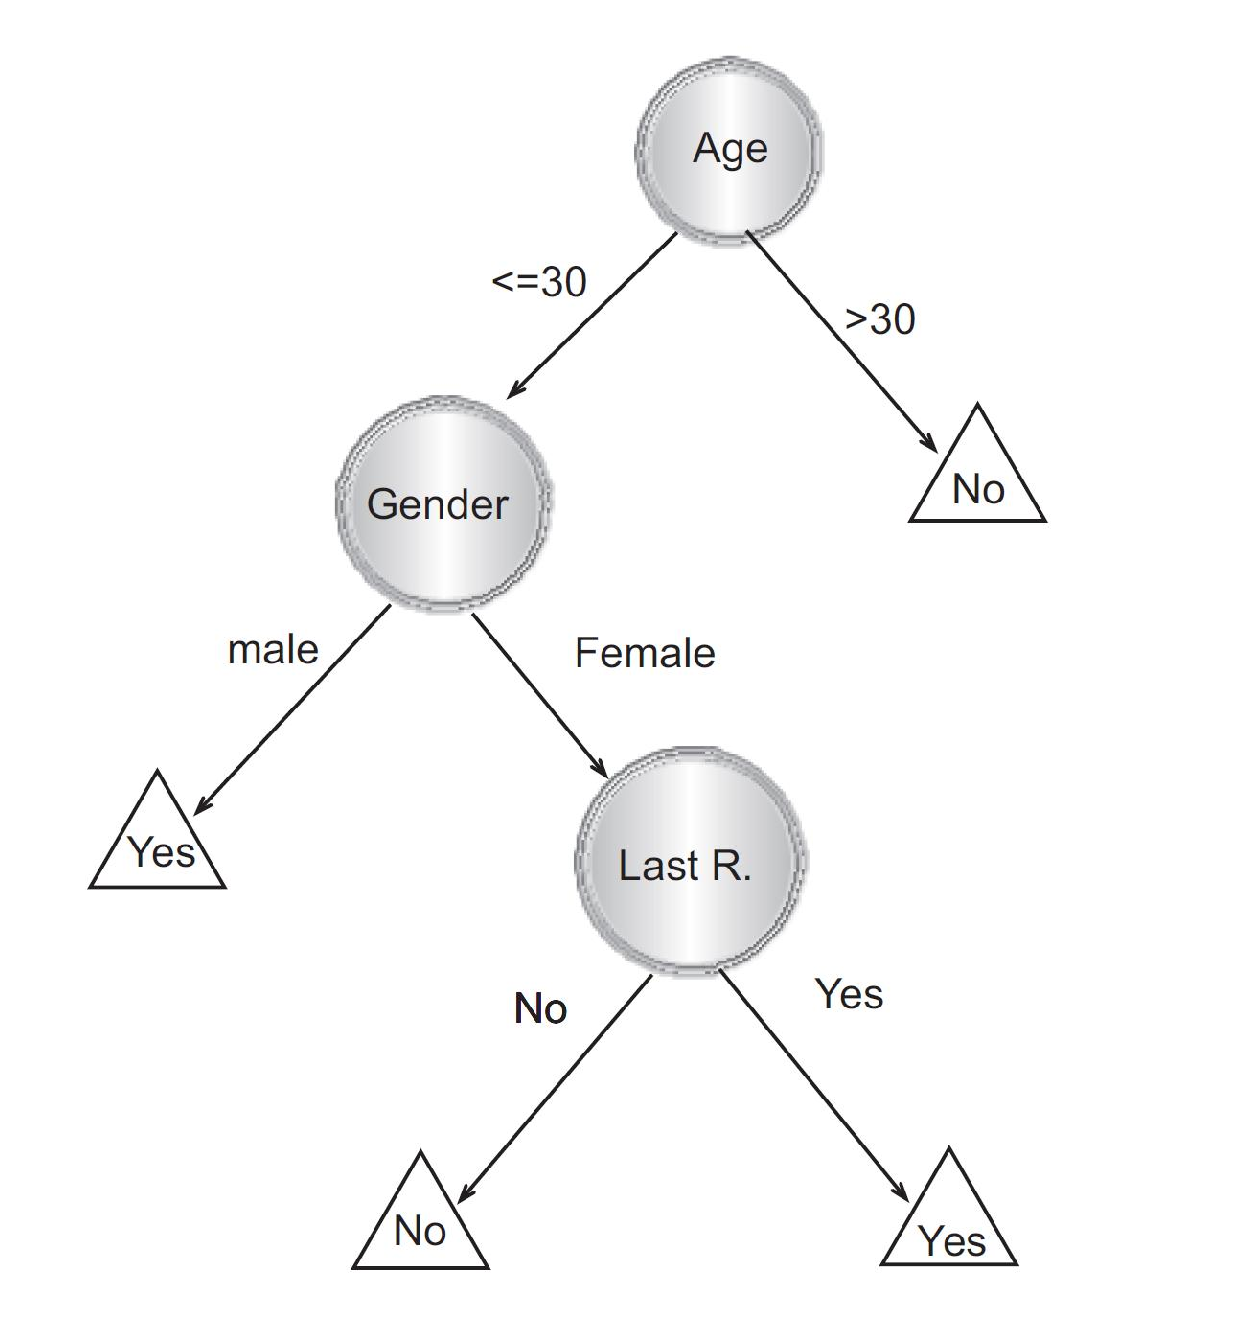
\includegraphics[width=0.6\linewidth]{images/chapter2/decision_tree.pdf}
	\caption{Drzewo decyzyjne \cite{rokach2007data}}
	\label{fig:decision-tree}
\end{figure}
Budowa drzewa decyzyjnego odbywa się typowo za pomocą algorytmu zachłannego. W danym wierzchołku wybierany jest ten atrybut oraz takie zakresy, które w wyniku podzielenia zbioru wejściowego stworzą podzbiory możliwie najbardziej jednorodne ze względu na klasy w nich zawarte. Ściślej, jako metrykę jakości danego podziału stosuje się zwykle miarę \textit{Information Gain} bądź \textit{Gini Impurity} --- wybór konkretnej miary jest hiperparametrem algorytmu uczącego, jednakże publikacje wskazują na to, że obie miary dają podobne wyniki \cite{tangirala2020evaluating}. Utworzone podzbiory przekazywane są rekurencyjnie w głąb drzewa w celu utworzenia kolejnych potomków. Procedura trwa do momentu gdy w każdym wierzchołku są już próbki z tylko jednej klasy, lub gdy zostanie osiągnięta maksymalna głębokość drzewa --- hiperparametr algorytmu.
Jak widać z konstrukcji modelu, drzewo decyzyjne ma bardzo wysoką interpretowalność --- łatwo zrozumieć w jaki sposób obliczona została dana predykcja. Drzewo decyzyjne charakteryzuje się też tym, że ma możliwość idealnego dopasowania się do danych treningowych. Często skutkuje to przeuczeniem się (\textit{overfitting}) i słabymi wynikami na danych testowych.

\subsection{Konstrukcja lasu losowego}

Las losowy budowany jest poprzez stworzenie pewnej liczby drzew decyzyjnych --- liczba drzew jest hiperparametrem algorytmu. Każde z drzew jest budowane na podstawie losowo stworzonego podzbioru zbioru treningowego. Ściślej, używana jest technika o nazwie \textit{bagging} (od ang. \textit{Bootstrap aggregating}) \cite{breiman1996bagging} --- dla zbioru wejściowego o rozmiarze $n$, dla każdego drzewa losowane jest ze zwracaniem $n$ próbek ze zbioru.
\\Dodatkowo, podczas budowy pojedynczych drzew, przy wybieraniu atrybutu do podziału w węźle drzewa, każdorazowo przeglądany jest jedynie losowy podzbiór atrybutów. Typowo losuje się $\sqrt{p}$ gdzie p to liczba atrybutów.
\\Tak zbudowany las wykorzystuje się do predykcji w następujący sposób --- dla danej próbki oblicza się predykcję z każdego z drzew, a następnie sprawdza się która z klas została przewidziana najczęściej.

\subsection{Właściwości}

Las losowy ma podobną siłę wyrazu jak drzewo decyzyjne. Jest jednak dużo bardziej odporny na przeuczenie --- innymi słowy ma mniejszą wariancję ale podobne obciążenie (\textit{bias}). Dzieje się tak dzięki temu, że drzewa są trenowane niezależnie --- czyni to model dużo mniej czułym na szum w zbiorze treningowym. Używanie podzbioru atrybutów podczas budowy węzłów ma za zadanie dodatkowego zmniejszenia korelacji między drzewami (w przeciwnym przypadku wszystkie stworzone drzewa będą preferowały atrybuty będące najsilniejszymi predyktorami, co sprawi, że będą one podobne) \cite{ho2002data}.
\\Las losowy jest też używany dla oszacowania ważności poszczególnych atrybutów --- podczas konstrukcji drzew, można zaobserwować jaka była miara jednorodności atrybutów użytych w węzłach. Tak stworzony ranking ważności atrybutów może pomóc w zinterpretowaniu zbioru danych, lub w wyborze najważniejszych atrybutów do innego algorytmu.

\subsection{Implementacja}

W ramach niniejszej pracy użyłyśmy implementacji lasu losowego dla języka Python zawartej w klasie \verb_sklearn.ensemble.RandomForestClassifier_ z biblioteki \verb_scikit-learn_. Pozwala ona na zdefiniowanie kluczowych hiperparametrów oraz na ekstrakcję ważności atrybutów.


\subsubsection {Wybór hiperparametrów}
\label{subsub: hyperparameters}

Do znalezienia hiperparametrów modelu (liczba drzew, maksymalna głębokość pojedynczego drzewa) użyłyśmy klasy \verb_RandomizedSearchCV_ z biblioteki
\verb_sklearn_ z pakietu \verb_model_$\_$\verb_selection_, która pozwala na przeszukiwaniu przestrzeni hiperparametrów na zdefiniowanym przez nas zakresie w efektywny sposób przy użyciu techniki walidacji krzyżowej (\textit{cross-validation}). Technika ta polega na wydzieleniu części danych treningowych, wytrenowaniu na nich modelu a następnie sprawdzeniu wyników predykcji na pozostałej części danych treningowych (zbiorze walidacyjnym). 

Użyta przez nas metoda używa techniki \textit{5-fold cross validation}, która polega na podzieleniu danych treningowych na 5 części, a następnie pięciokrotnym powtórzeniu procedury walidacji krzyżowej (tak, aby każda z 5 części raz została użyta jako zbiór walidacyjny). Wyniki wszystkich eksperymentów są zapisywane w klasie wraz z ich najistotniejszymi miarami statystycznymi (średnia wyników, odchylenie standardowe, średni czas trenowania modelu) oraz rankingowane.
\\\verb_RandomizedSearchCV_ jest przydatnym narzędziem, gdy chcemy przeszukać duży zbiór hiperparametrów i czas trenowania modelu jest długi. Nie sprawdza ona wszelkich możliwych kombinacji, tylko trenuje model na losowo wybranych hiperparametrach z podanych przez nas przedziałów, rozkładów lub zbiorów. 


\section{Maszyna wektorów nośnych}
\label{sec:svm}

Maszyna wektorów nośnych (\textit{Support Vector Machine}, SVM) \cite{cortes1995support}, jest to jeden z klasycznych algorytmów klasyfikacji binarnej. Opiera się on na znalezieniu hiperpłaszczyzny rozdzielającej przestrzeń danych wejściowych na dwie klasy, w taki sposób by odległość punktów danych od hiperpłaszczyzny była jak największa.

W tej sekcji opisana jest konstrukcja maszyny wektorów nośnych, następnie opisane są właściwości modelu, a na końcu szczegóły implementacji algorytmu na potrzeby niniejszej pracy.

\subsection{Konstrukcja}

Dane wejściowe o $p$ atrybutach można traktować jako zbiór punktów w $p$-wymiarowej przestrzeni --- każdy o przypisanej klasie. Maszyna wektorów nośnych to metoda znalezienia takiej $(p-1)$-wymiarowej płaszczyzny, która będzie rozdzielać punkty z jednej klasy od punktów z drugiej klasy. W przypadku gdy istnieje wiele takich płaszczyzn, wybierana jest taka, która maksymalizuje odległość najbliższych jej punktów. W przypadku gdy nie istnieje taka płaszczyzna, wybierana jest taka, która minimalizuje dodatkowo odległość od niej błędnie sklasyfikowanych punktów. To w jakim stosunku optymalizować te dwa cele jest hiperparametrem algorytmu (dalej oznaczony $\lambda$). 

\begin{figure}[H]
	\centering
	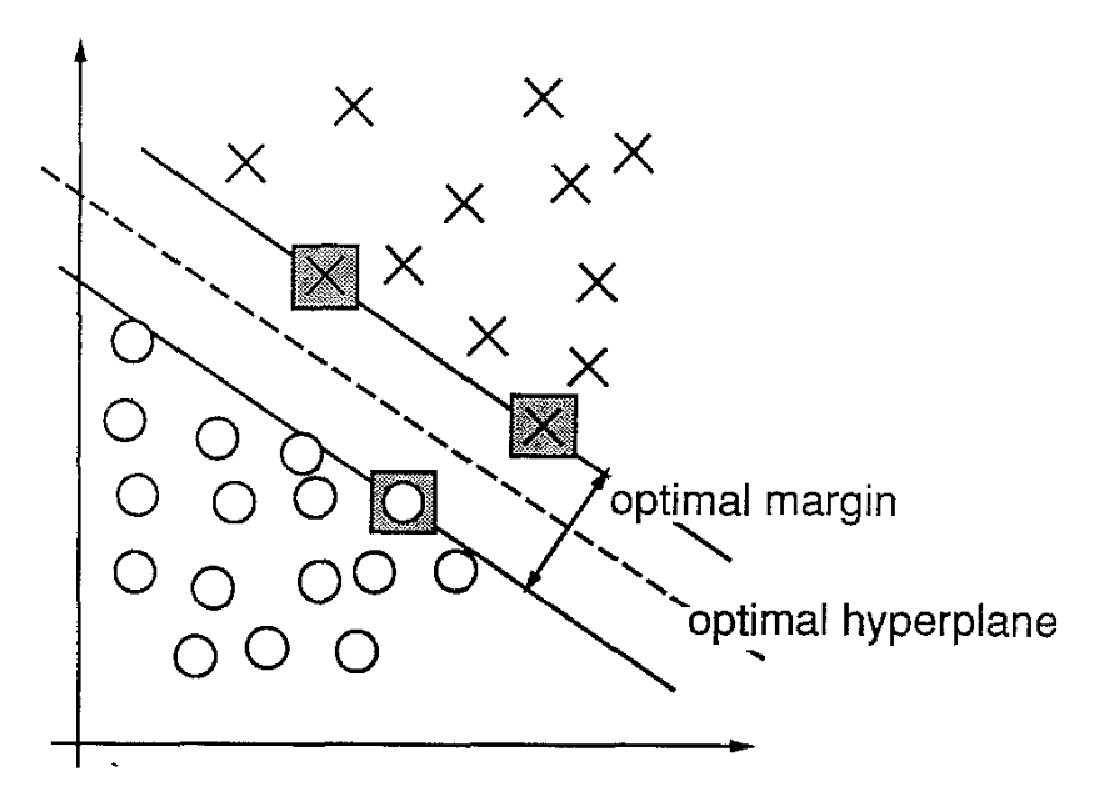
\includegraphics[width=0.6\linewidth]{images/chapter2/SVM.pdf}
	\caption{Przykład rozdzielonych punktów w 2-wymiarowej przestrzeni --- wektory nośne oznaczone są kwadratami \cite{cortes1995support}}
	\label{fig:svm}
\end{figure}
\noindent Wyraźmy hiperpłaszczyznę za pomocą jej wektora normalnego w oraz liczby $b$:
\begin{equation}
w^Tx - b = 0 
\end{equation}

\noindent Znalezienie odpowiedniej hiperpłaszczyzny sprowadza się do minimalizacji funkcji kosztu $f(w,b)$
\begin{equation}
\left[ \frac{1}{n}\sum_{i=1}^n \max(0, 1 - y_{i}(w^Tx_{i} - b))\right] + \lambda ||w|| ^2
\end{equation}

\noindent gdzie $n$ to liczba punktów, $x_i$ to $i$-ty punkt danych, $y_i$ to wartość jego klasy ($1$ lub $-1$), a $\lambda$ to hiperparametr algorytmu.
\\Pierwszy człon wyraża karę za źle sklasyfikowane punkty (tym większą im dalej są od hiperpłaszczyzny). Drugi człon jest odwrotnie proporcjonalny do kwadratu odległości hiperpłaszczyzny od poprawnie sklasyfikowanych punktów.

\subsection{Właściwości}

Maszyna wektorów nośnych w opisanej postaci tworzy model liniowy, charakteryzuje się więc wysokim obciążeniem (\textit{bias}) i niską wariancją. W sytuacjach gdzie klasy nie są łatwo separowalne liniowo, często stosuje się tzw. kernel trick przekształcający nieliniowo oryginalną przestrzeń punktów \cite{aizerman1964theoretical}.

\subsection{Implementacja}

W ramach niniejszej pracy użyłyśmy klasycznej implementacji maszyny wektorów nośnych dla języka Python zawartej w klasie \verb_sklearn.svm.LinearSVC_ z biblioteki \verb_scikit-learn_. Pozwala ona na zdefiniowanie hiperparametru $C = 1/ \lambda$.
\\Do znalezienia parametru \textit{C} użyłyśmy klas z biblioteki \verb_sklearn.model_$\_$\verb_selection_ - \verb_RandomizedSearchCV_ opisanej powyżej (Sekcja. \ref{subsub: hyperparameters}) oraz \verb_GridSearchCV_  
która również używa techniki walidacji krzyżowej, jednak sprawdza wszystkie możliwe kombinacje ze zdefiniowanych przez nas zbiorów. 


\section{Konwolucyjna sieć neuronowa}
\label{sec:cnn}
Konwolucyjna sieć neuronowa (\textit{Convolutional Neural Network}) to rodzaj sztucznej sieci neuronowej. Jej konstrukcja jest inspirowana procesami biologicznymi zachodzącymi w korze wzrokowej w mózgu \cite{chauhan2018convolutional}. Typowo sieci konwolucyjne wykorzystuje się do zadań uczenia maszynowego związanego z rozpoznawaniem obrazów. Mogą być jednak stosowane także w innych dziedzinach, w szczególności w przetwarzaniu języka naturalnego.

W tej sekcji najpierw opisany jest koncept klasycznej sieci neuronowej. Następnie opisana jest konstrukcja konwolucyjnej sieci, oraz zastosowanie jej w przetwarzaniu języka naturalnego. Na końcu podane są szczegóły implementacji sieci na potrzeby niniejszej pracy.

\subsection{Sieci neuronowe}
\label{subsec:nn}

Klasyczna wielowarstwowa sieć neuronowa składa się z sekwencji warstw, w których znajduje się duża liczba węzłów obliczeniowych (tzw. neuronów). Pojedynczy neuron przyjmuje na wejściu wektor liczb rzeczywistych $x$, do którego następnie aplikowany jest wektor wag $w$ (wynik uczenia sieci) przypisany do tego neuronu.
W wyniku otrzymywana jest liczba:

\begin{equation}
a = \sum_{i=1}^n w_i x_i
\end{equation}

\noindent do której aplikowana jest funkcja aktywacji --- decydująca o tym, jaki wynik zostanie przekazany do kolejnej warstwy \cite{gurney2013introduction}. Funkcje aktywacji odgrywają ważną rolę w sieciach neuronowych --- pozwalają dodać nieliniowość --- bez ich użycia, wynik wyjściowy modelu byłby kombinacją liniową danych wejściowych, z ograniczonymi możliwościami modelowania skomplikowanych typów danych (takich jak obrazy czy język naturalny) \cite{sharma2017activation}.  

\begin{figure}[H]
	\centering
	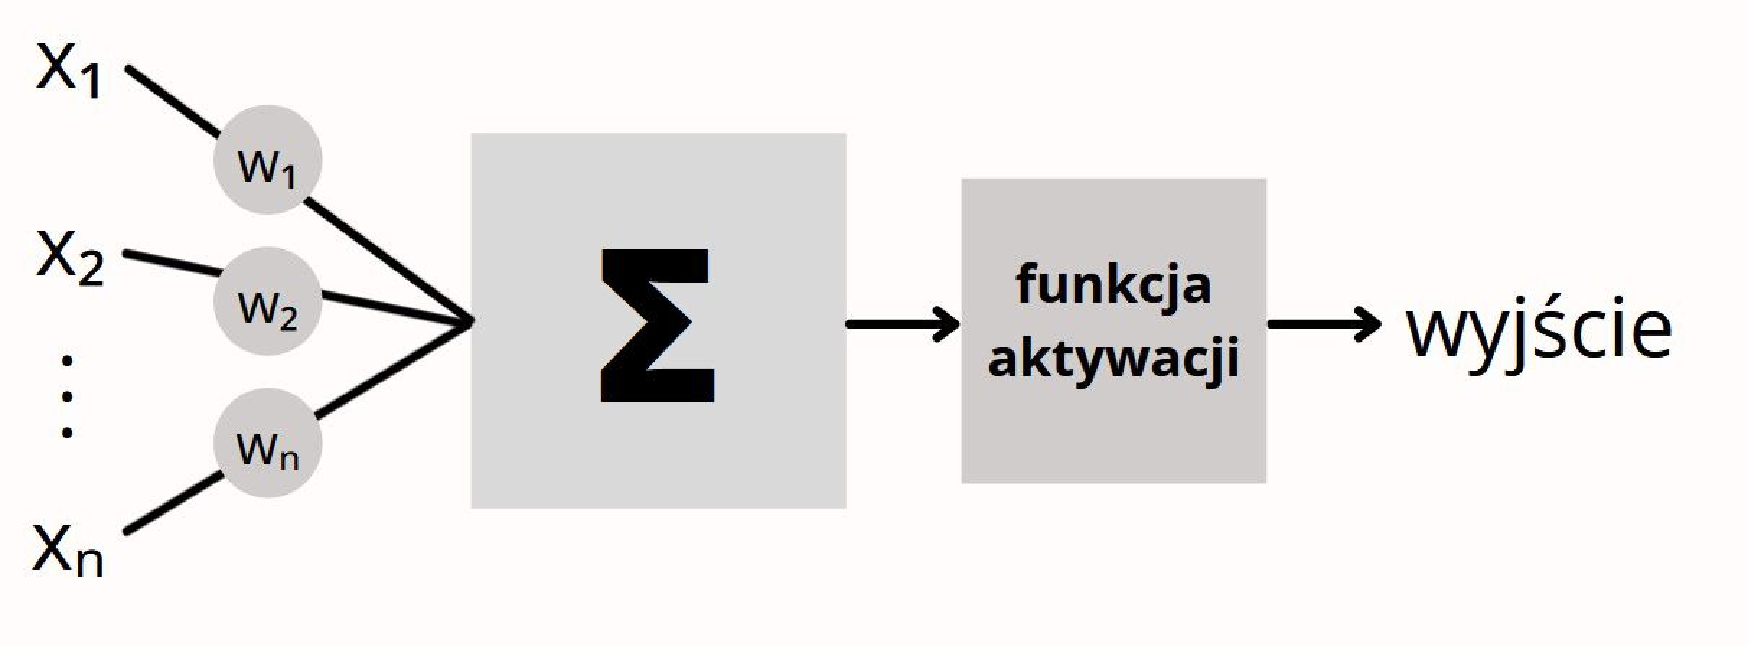
\includegraphics[width=0.6\linewidth]{images/chapter2/perceptron.pdf}
	\caption{Schemat działania pojedynczego neuronu}
	\label{fig:perceptron}
\end{figure}

\noindent Pierwsza warstwa nazywana jest warstwą wejściową (\textit{input layer}), która przyjmuje na wejściu czyste dane w postaci wektorów. Kolejne warstwy to warstwy ukryte (\textit{hidden layers}), do których wejściami są wyniki przekazane przez neurony poprzedniej warstwy. Ostatnią warstwą jest warstwa wyjściowa (\textit{output layer}), która na wejściu również przyjmuje dane z poprzedniej warstwy, a której wyjcie jest predykcją modelu.

\begin{figure}[H]
	\centering
	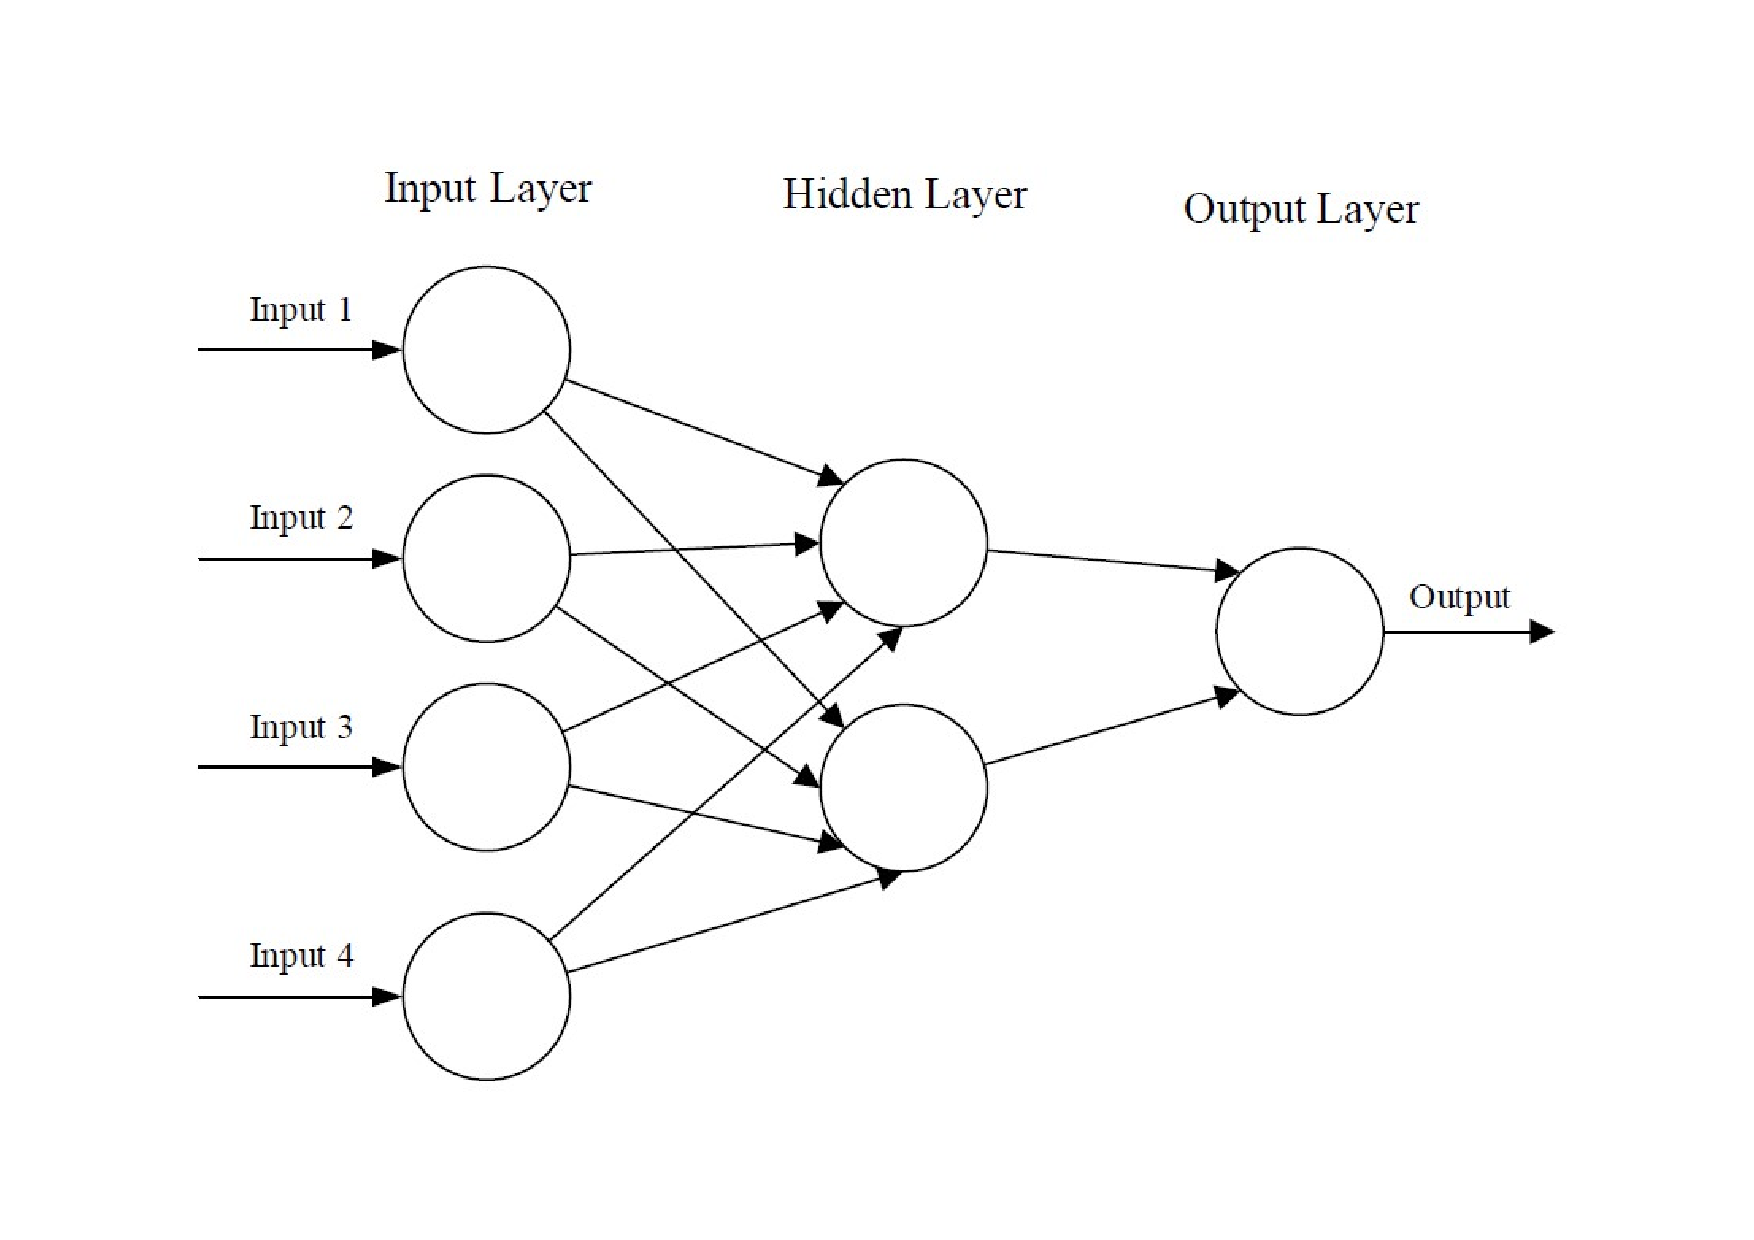
\includegraphics[width=0.9\linewidth]{images/chapter2/ann-layers.pdf}
	\caption{Wielowarstwowa sieć neuronowa \cite{o2015introduction}}
	\label{fig:ann-layer}
\end{figure}

\noindent Istnieje wiele różnych funkcji aktywacji, z których najpopularniejsze opisane są w \cite{sharma2017activation}. W ramach niniejsze pracy wykorzystałyśmy następujące funkcje:
\begin{enumerate}
	\item Funkcja sigmoidalna
	\begin{equation}
	f(x) = \frac{1}{1 + e^{-x}}
	\end{equation}
	
	Funkcja ta, mapująca liczby rzeczywiste na przedział $(0, 1)$, jest jedną z najczęściej stosowanych w sieciach neuronowych.
	
	\item Funkcja ReLU (od ang. \textit{rectified  linear  unit}) 
	\begin{equation}
	f(x) = \max(0,x)
	\end{equation}
	
	Funkcja ta jest szeroko stosowana w warstawch ukrytych m.in. dzięki prostocie obliczeń oraz rozrzadzeniu aktywnych neuronów (neurony aktywują się tylko dla $a > 0$).
	
\end{enumerate}

\subsection{Trening sieci neuronowej}

Trening --- uczenie sieci neuronowej ma na celu zminimalizowanie obserwowanego błędu, czyli różnicy między predykcją sieci na danych treningowych a faktycznymi klasami. Sieć inicjalizuje się z losowymi wagami. Następnie sieć jest aplikowana do danych wejściowych i wagi są aktualizowane w celu zmniejszeniu uzyskanego błędu. Proces powtarzany jest iteracyjnie. \cite{gurney2013introduction}. Hiperparametrami modelu są liczba iteracji (epok) oraz ile próbek naraz używać podczas jednego kroku aktualizacji (wielkość wsadu, \textit{batch size}).
\\Aktualizacja wag odbywa się za pomocą procesu zwanego propagacją wsteczną (\textit{backpropagation})  \cite{goodfellow2016deep}. Wagi aktualizowane są w kierunku gradientu funkcji błędu w zależności od tych wag. Innymi słowy, wartość błędu jest dzielona proporcjonalnie pomiędzy wagi które za niego odpowiadają.
\\W celu przeciwdziałania przeuczeniu się sieci neuronowej, można wykorzystać technikę zwaną \textit{dropout} \cite{srivastava2014dropout}. Polega ona na zignorowaniu podczas obliczania predykcji na potrzeby treningu niektórych neuronów z prawdopodobieństwem $p$ będącym hiperparametrem. Dzięki temu że żaden neuron nie jest trenowany na całym zbiorze treningowym, sieć będzie miała mniejszą skłonność do przeuczenia się.

\subsection{Sieci konwolucyjne}
\label{subsec:cnn}

Sieci konwolucyjne są modyfikacją sieci neuronowych, stworzone z myślą o przetwarzaniu obrazów. Wejściem do sieci konwolucyjnej jest trójwymiarowa macierz: typowo jest to dwuwymiarowy obrazek, gdzie każdy piksel opisany jest trzema wartościami --- R, G, B. Podobnie jak w przypadku sieci neuronowych, sieć konwolucyjna składa się z sekwencji warstw.

Pojedyncza warstwa konwolucyjna składa się z pewnej liczby (hiperparametr) filtrów. Każdy filtr to trójwymiarowa macierz wag. Wysokość i szerokość filtra (hiperparametry) powinny być mniejsze niż odpowiednio wysokość i szerokość wejścia, natomiast głębokość musi być równa głębokości wejścia. Zaaplikowanie filtru do macierzy wejściowej polega na “przyłożeniu” go do każdej możliwej pozycji $x$,$y$ wejścia, i obliczeniu iloczynu skalarnego filtra i odpowiedniego wycinka wejścia. W wyniku tej aplikacji powstaje dwuwymiarowa macierz zawierająca iloczyny skalarne, o wysokości i szerokości równych wysokości i szerokości wejścia (aby nie tracić informacji o pikselach znajdujących się na rogach obrazkach, często stosuje się technikę nazywaną \textit{zero-padding} --- jej szczegółowy opis można znaleźć w \cite{albawi2017understanding}. Wyniki aplikacji wszystkich filtrów z warstwy razem tworzą macierz trójwymiarową, która służy jako wejście do kolejnej warstwy.

\begin{figure}[H]
	\centering
	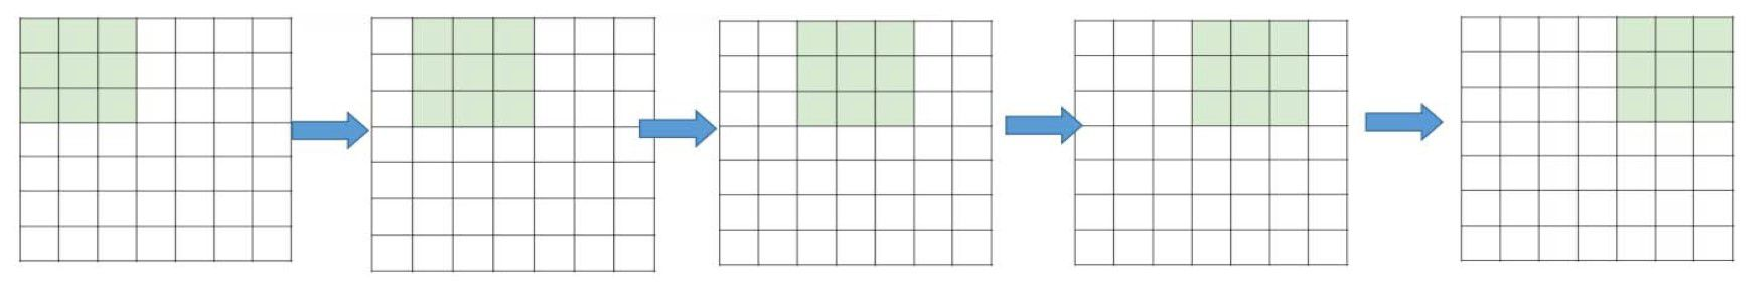
\includegraphics[width=0.8\linewidth]{images/chapter2/filter.pdf}
	\caption{Zastosowanie filtra w sieci konwolucyjnej \cite{albawi2017understanding}}
	\label{fig:filter}
\end{figure}

\noindent Oprócz warstw konwolucyjnych, stosuje się też inne rodzaje warstw. Jedną z nich jest warstwa typu \textit{pooling}. Jej zadaniem jest zmniejszenie wymiarowości danych płynących przez sieć. W tym celu segmenty wejścia są agregowane, na przykład poprzez branie maksimum z ich wartości \cite{albawi2017understanding}.

Architektura sieci konwolucyjnej typowo składa się z kilku warstw konwolucyjnych przeplatanych z warstwami \textit{pooling}, a następnie kilku warstw klasycznych sieci neuronowych, w tym kontekście nazywanych warstwami \textit{fully connected}. Trójwymiarowa macierz wychodząca z warstwy konwolucyjnej jest spłaszczana do jednowymiarowego wektora w celu przekazania jej do warstwy \textit{fully connected}.

\begin{figure}[H]
	\centering
	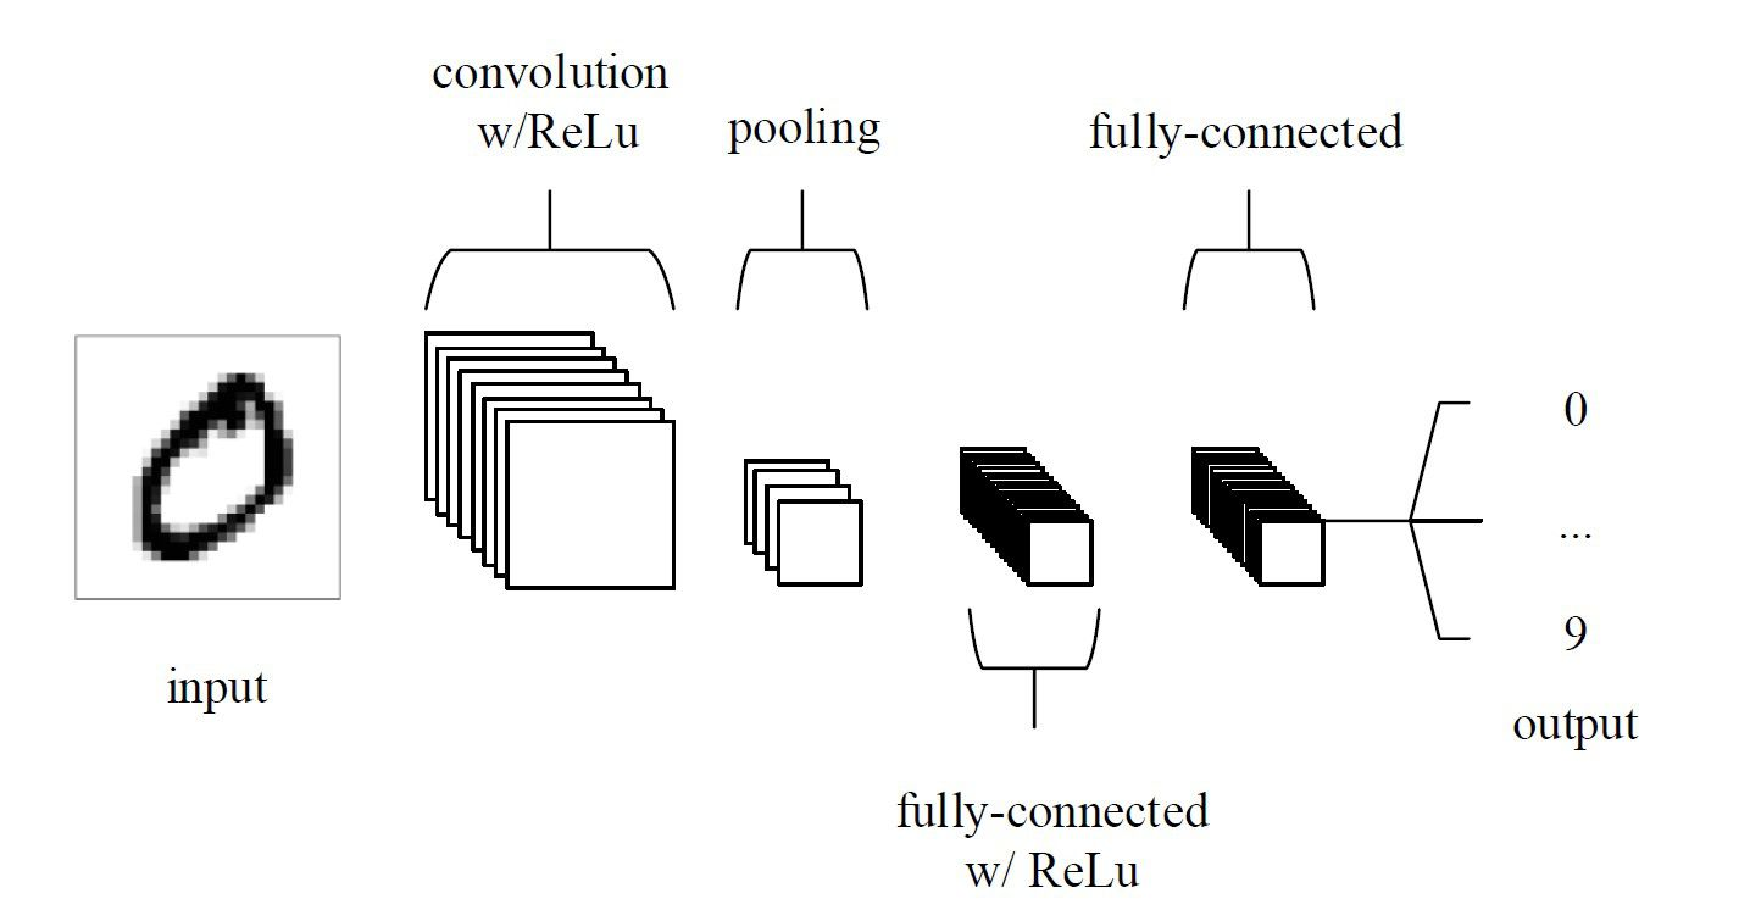
\includegraphics[width=0.8\linewidth]{images/chapter2/layered-conv.pdf}
	\caption{Pięciowarstwowa sieć konwolucyjna \cite{o2015introduction}}
	\label{fig:layered-conv}
\end{figure}

\subsection{Wykorzystanie sieci konwolucyjnych w przetwarzaniu języka naturalnego}
\label{subsec:word2vec}

Choć sieci konwolucyjne wymyślone zostały z intencją przetwarzania obrazów, w ostatnich latach wielokrotnie były wykorzystywane do przetwarzania tekstu \cite{minaee2019deep}. Wymaga to najpierw zanurzenia (\textit{embedding}) słów --- wyrażenia każdego słowa w postaci wektora liczb. Można wykorzystać do tego metodę Word2Vec \cite{mikolov2013efficient}. Polega ona na wytrenowaniu sieci neuronowej na korpusie tekstów, która dla danego słowa zwraca wektor liczb. Sieć trenowana jest w ten sposób, by wektory słów występujących w podobnym kontekście znajdowały się blisko siebie.

\begin{figure}[h]
	\centering
	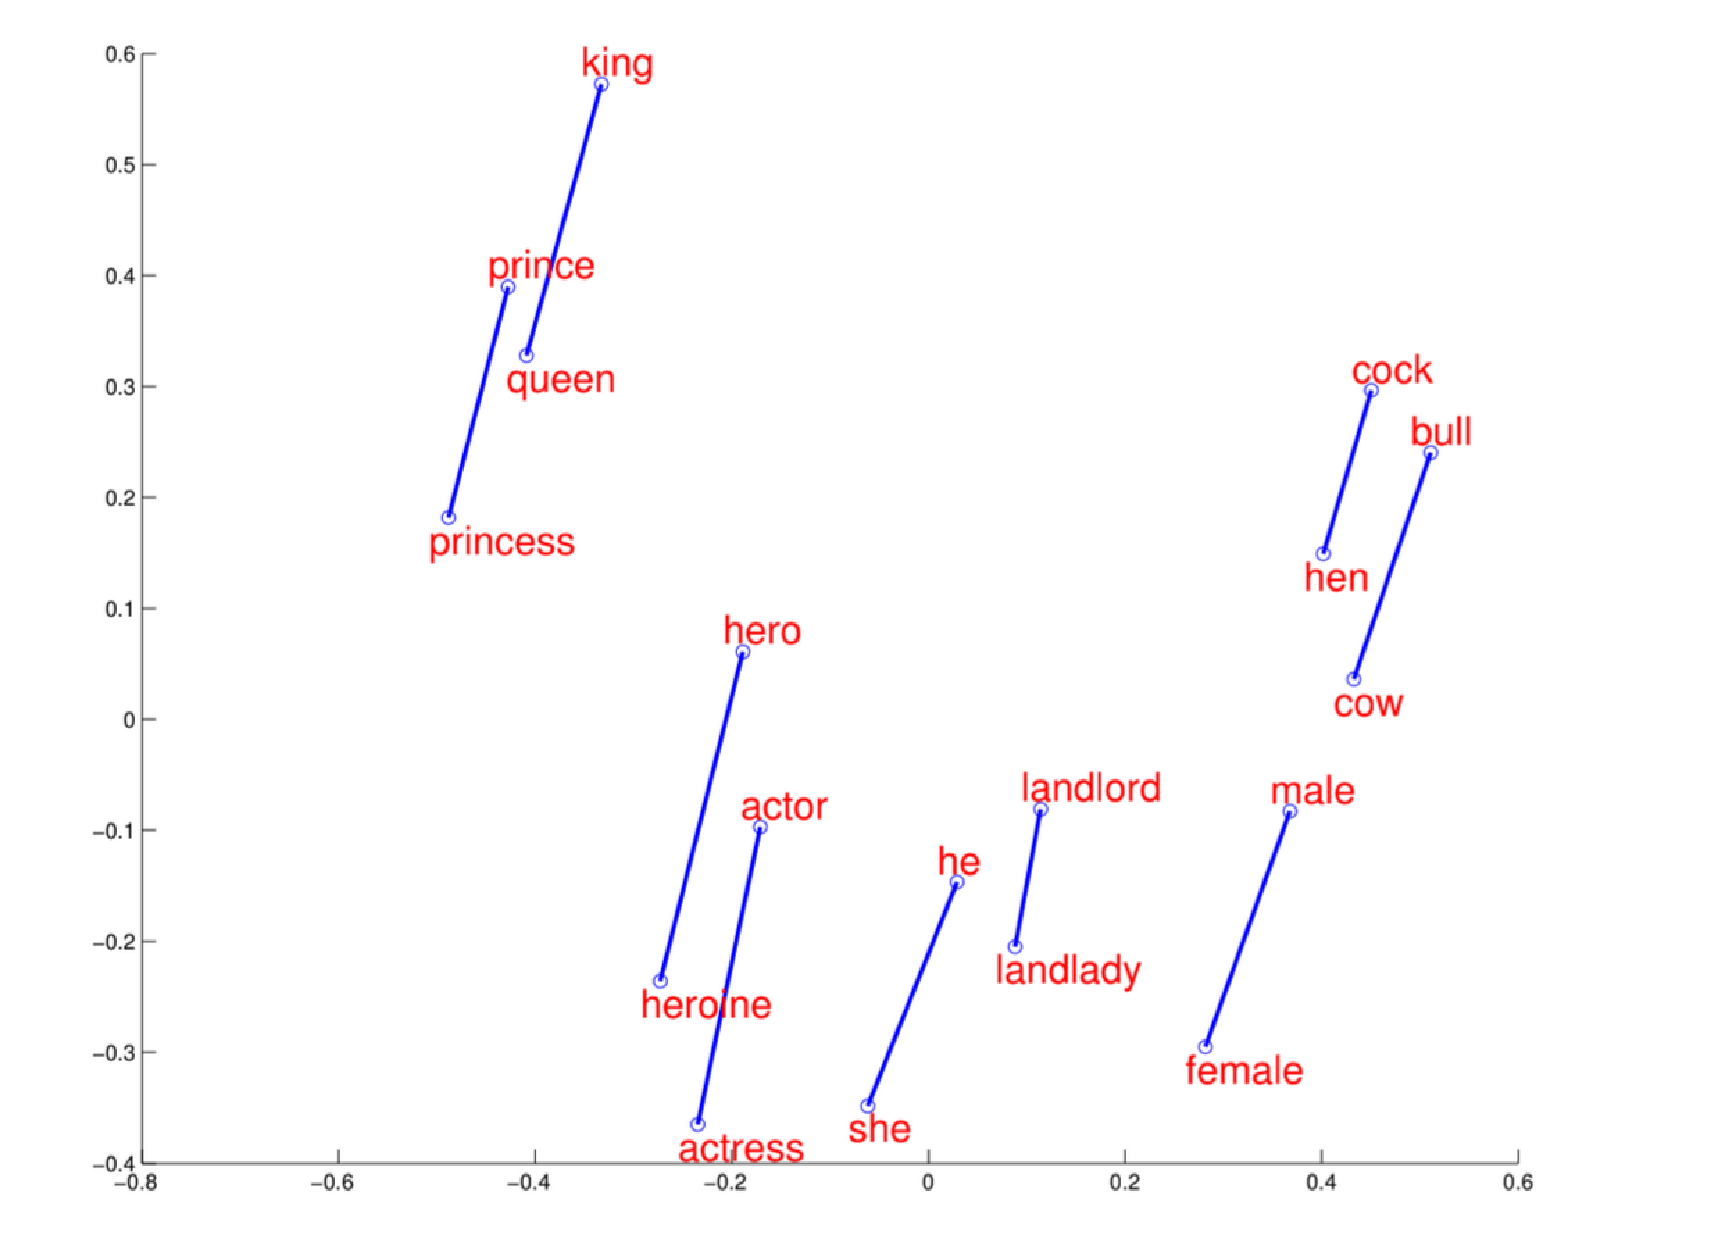
\includegraphics[width=0.8\linewidth]{images/chapter2/w2vpng.pdf}
	\caption{\href{https://drive.google.com/file/d/0B7XkCwpI5KDYRWRnd1RzWXQ2TWc/edit?resourcekey=0-oGRnY6qG7yWEqCXOHFKPcw}
		{Wizualizacja działania metody Word2vec}}
	\label{fig:word2vec}
\end{figure}

W przypadku tekstu, wejściem dla sieci konwolucyjnej będzie macierz nie trójwymiarowa, a dwuwymiarowa. Zamiast dwuwymiarowego obrazu używany jest jednowymiarowy tekst. Podczas gdy w przypadku obrazów każdy piksel reprezentowany jest za pomocą trzech liczb (R, G, B), każde słowo tekstu wejściowego jest wyrażone odpowiadającym mu wektorem zanurzenia.

W przypadku obrazów, pojedynczy filtr aplikowany jest do pikseli znajdujących się blisko siebie. Intuicyjnie, każdy piksel należy interpretować w kontekście jego otoczenia. W przypadku tekstów, analogicznie filtr aplikowany jest do słów znajdujących się blisko siebie. Jedyną różnicą jest że dla obrazów otoczenie ma dwa wymiary --- szerokość i wysokość, zaś dla tekstów jest to tylko jeden wymiar.

\subsection{Implementacja}

\subsubsection{Word2Vec}
\label{subsubsec:w2v}

W niniejszej pracy w stworzenia wektorów używanych do reprezentacji słów w nazszych modelach użyłyśmy implementacji algorytmu w języku Python zawartej w klasie \verb_gensim.models.Word2Vec_ z biblioteki \verb_gensim_. 
\\Zdecydowałyśmy się na własne wytrenowanie modelu na słowniku z danych treningowych, w związku z tym, że konktekst słów używanych w recenzjach filmowych często różni się od tych wykorzystywanych w różnego rodzaju artykułach (na których zazwyczaj trenowane są dostępne modele).

\subsubsection{Sieć konwolucyjna} 

W ramach niniejszej pracy wykorzystałyśmy bibliotekę \verb_keras_, która jest jedną z najczęściej używanych deep-learningowych bibliotek w języku Python. Pozwala ona na proste dodawanie kolejnych warst sieci, w celu tworzenia skomplikowanych modeli.
Do implementacji sieci konwolucyjnej użyłyśmy następujących funkcji:

\begin{itemize}
	\item \verb_keras.models.Sequential_ budowanie modelu, do którego następnie dodawane są kolejne warstwy. Kolejne sekwencje warstw na wejściu przyjmują wyjścia z warstw poprzednich.
	
	\item \verb_keras.layers.Embedding_ pierwsza warstwa modelu, której wejściem jest lista słów treningowych oraz sposób ich wektoryzacji (wynik działania modelu Word2vec), a wyjściem słowa przetłumaczone na wektory
	
	\item \verb_keras.layers.Conv1D_ warstwa konwolucyjna  aplikująca filtry o wysokości $1$
	
	\item \verb_keras.layers.GlobalMaxPooling1D_ warstwa typu \textit{pooling}, biorąca maksymalną wartość z dla każdego filtra 
	
	\item \verb_keras.layers.Dropout_ warstwa wykorzystana w celu zapobiegnięcia przetrenowania sieci
	
	\item \verb_keras.layers.Dense_ kolejnymi warstwami są tzw. warstwy \textit{fully-connected}. 
	
\end{itemize}


\section{Sieć LSTM}
\label{sec:lstm}

Długoterminowa pamięć krótkoterminowa (\textit{Long short-term memory}, dalej LSTM) to rekurencyjna sieć neuronowa. Została zaprojektowana z myślą o przetwarzaniu wejścia o zmiennej długości. Wejście do sieci przetwarzane jest sekwencyjnie --- wyjście z sieci dla dotychczasowo przetworzonej sekwencji wpływa na zachowanie modelu dla dalszej części sekwencji. Dzięki temu LSTM bardzo dobrze nadaje się do przetwarzania tekstu.

W tej sekcji najpierw przybliżony jest koncept rekurencyjnej sieci neuronowej, następnie opisana jest konstrukcja sieci LSTM oraz jej zastosowanie w przetwarzaniu języka naturalnego. Na końcu podane są szczegóły implementacji sieci na potrzeby niniejszej pracy.

\subsection{Rekurencyjna sieć neuronowa}
\label{subsec:rnn}

Rekurencyjne sieci neuronowe są typem sieci neuronowych specjalizujących się w przetwarzaniu sekwencji danych \cite{goodfellow2016deep}. 
W rekurencyjnej sieci neuronowej, neurony są połączone w sposób tworzący skierowany cykl. Jako wejście sieć przyjmuje sekwencję elementów --- na przykład wektory reprezentujące kolejne słowa tekstu. Aplikacja sieci rekurencyjnej dla danej sekwencji polega na wprowadzeniu do sieci po kolei każdego z elementów. Otrzymane wyjście sieci --- wektor stanu --- jest każdorazowo wprowadzany do niej wraz z kolejnym przetwarzanym elementem sekwencji. Ponadto, wektor stanu jest przetwarzany dodatkowymi neuronami w celu otrzymania kolejnego wektora wyjściowego. Zauważmy, że tak zdefiniowana sieć rekurencyjna pozwala uzyskać na wyjściu sekwencje o zmiennej długości. Jednak w przypadku klasyfikacji interesuje nas jedynie ostatni wektor wyjściowy.

\begin{figure}[H]
	\centering
	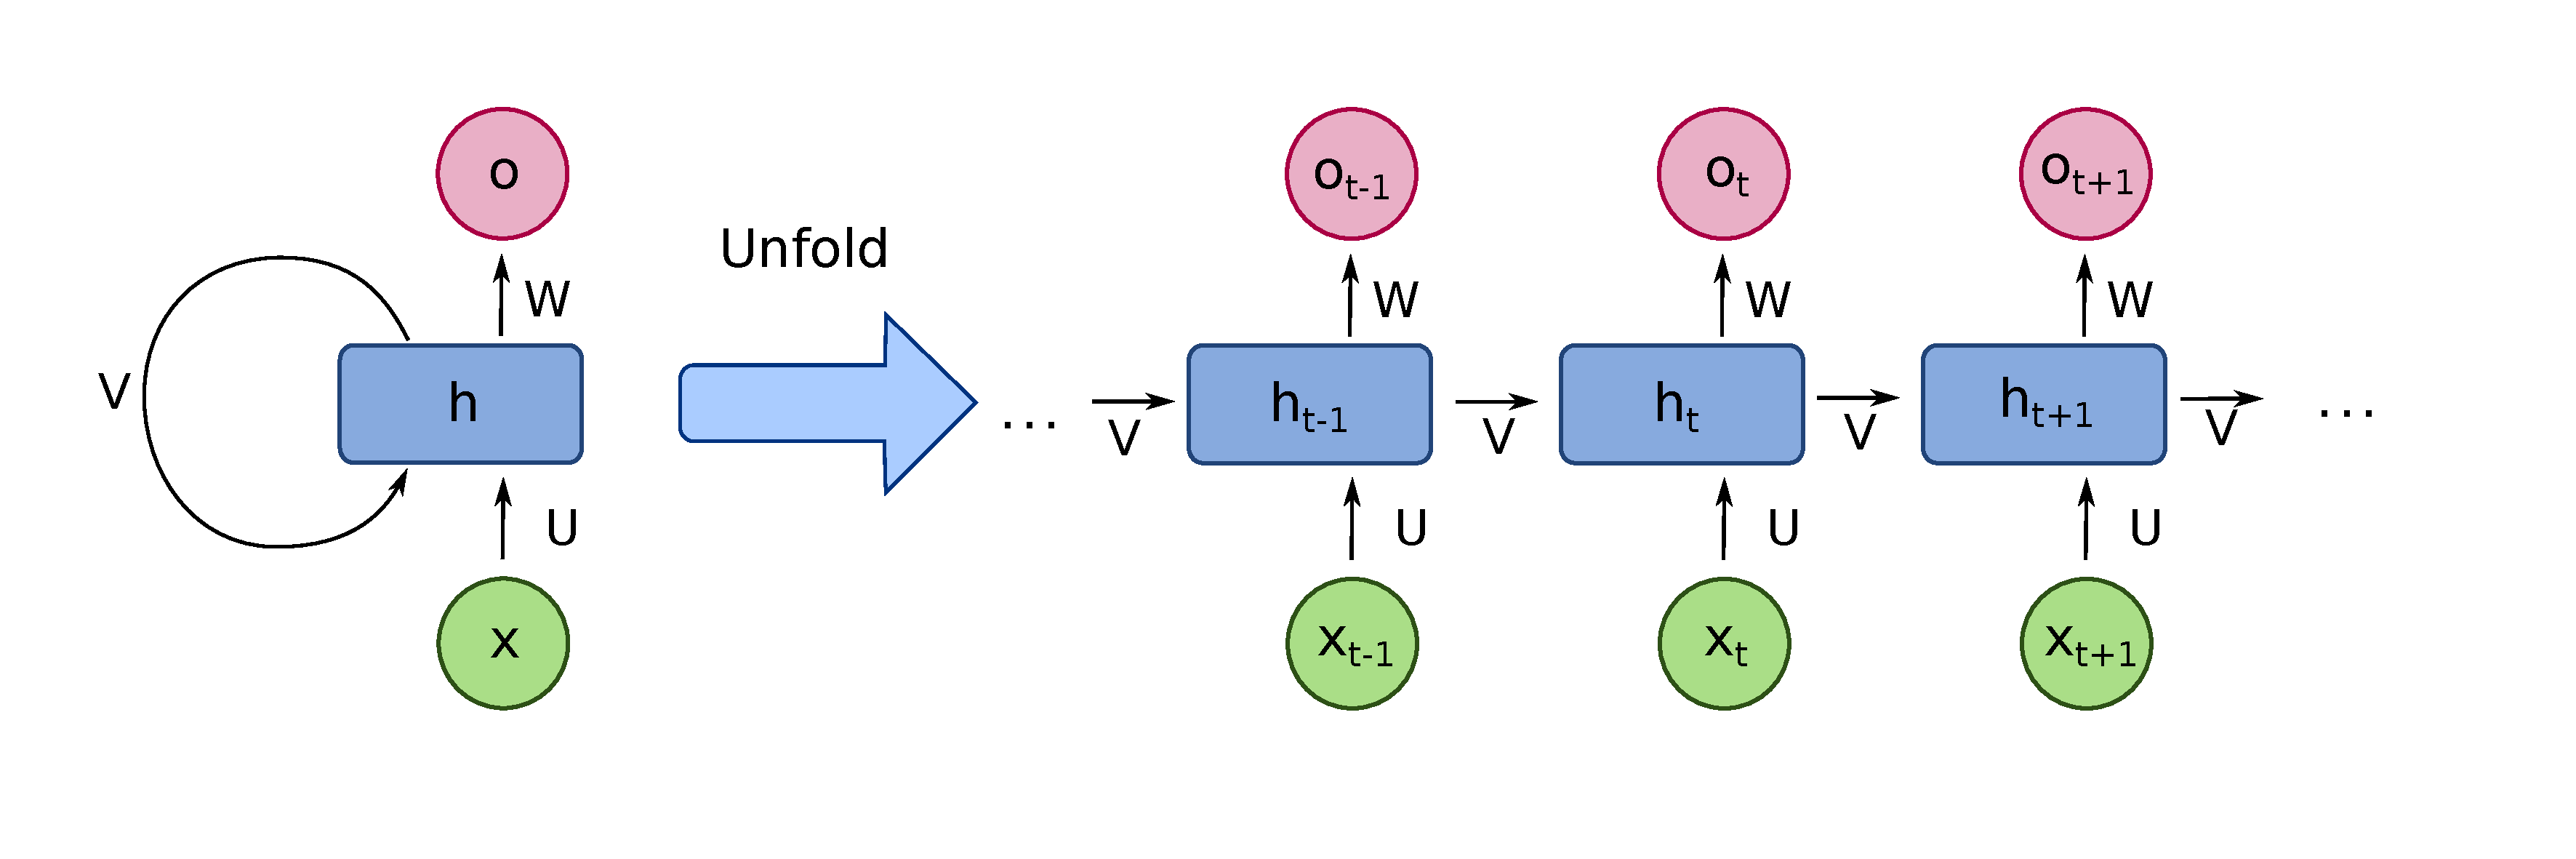
\includegraphics[width=0.95\linewidth]{images/chapter2/rnn.pdf}
	\caption{\href{https://commons.m.wikimedia.org/wiki/Artificial_neural_network} {Schemat działania rekurencyjnej sieci neuronowej z wektorem wejściowym $x$, wektorem wyjściowym $o$, wektorem stanu $h$ oraz macierzami wag $U, V, W$. Po lewej stronie przedstawiony został uprosznony model sieci, po prawej widzimy aplikację sieci dla kolejnych wektorów z sekwencji wejściowej}}
	\label{fig:rnn}
\end{figure}
\noindent Uczenie rekurencyjnej sieci neuronowej przebiega tak samo jak uczenie klasycznej sieci neuronowej, poprzez mechanizm propagacji wstecznej. Podczas uczenia sieci rekurencyjnej istnieje jednak duże ryzyko wystąpienia zjawiska zanikającego gradientu (\textit{vanishing gradient problem}) \cite{hochreiter1997long}. Problem ten może wystąpić także w klasycznych, nie rekurencyjnych sieciach neuronowych. Polega on na tym, że aktualizacje wag docierające do wcześniejszych (bliższych wejścia) warstw sieci stają się zbyt małe by znacząco zmienić jej zachowanie --- tym samym uniemożliwiając uczenie. W przypadku sieci rekurencyjnych problem jest bardziej dotkliwy, ponieważ dla przetworzenia całej sekwencji wejściowej są użyte te same wagi. Jeśli więc wagi te są mniejsze niż 1, dla wczesnych elementów sekwencji aktualizacje będą zbiegać do zera. (W przypadku wag większych niż 1, będą zbiegać do nieskończoności, co nazywane jest problemem eksplodującego gradientu). Konstrukcja LSTM opisana w następnej sekcji jest jednym ze sposobów przeciwdziałania temu zjawisku.

\subsection{Konstrukcja LSTM}

Model LSTM ma możliwość zapisania i odczytania stanu związanego z dawno przetworzonymi elementami wejściowymi. W kolejnych krokach aplikacji LSTM, oprócz dotychczasowego wyjścia przekazywany jest też wektor stanu pamięci. Po wczytaniu kolejnego elementu z sekwencji wejściowej, sieć może “zdecydować” czy odczytać informację z pamięci, czy ją nadpisać, i czy ją zresetować. Jest to zrealizowane poprzez specjalne bramki, które dla obecnego wejścia zwracają wartość 0 lub 1 (poprzez zaaplikowanie funkcji sigmoidailnej). Kolejna bramka oblicza jaką wartością nadpisać zawartość pamięci.

\subsection{Zastosowanie LSTM w przetwarzaniu języka naturalnego}

Zgodnie z jego oryginalnym przeznaczeniem, LSTM można zaaplikować do przetwarzania tekstów --- ciągów słów. Ponieważ na wejściu LSTM oczekuje sekwencji wektorów, tekst należy najpierw odpowiednio przetworzyć, na przykład za pomocą Word2Vec (Sekcja. \ref{subsec:word2vec}).

\subsection{Implementacja}

Tak jak w przypadku, wykorzystałyśmy tutaj bibliotekę \verb_keras_, poza opisanymi wcześniej funkcjami wykorzystałyśmy także dodatkową wartwę \verb_keras.layers.LSTM_. Implementuje ona rekurencyjną sieć LSTM, pozwala na zdefiniowanie wielkości wektora wyjściowego oraz prawdopodobieństwa \textit{dropoutu}.

\section{Połączenie sieci konwolucyjnej i LSTM}
\label{sec:cnn-lstm}

Częstym podejściem stosowanym w uczeniu maszynowym w celu poprawy jakości predykcji jest tzw. ensembling \cite{opitz1999popular}. Polega on na połączeniu wielu wytrenowanych modeli predykcyjnych w jeden. W publikacji \cite{minaee2019deep} autorzy opisują podejście w którym uśredniają predykcję z sieci konwolucyjnej oraz z modelu LSTM, uzyskując ostatecznie lepszy wynik na zbiorze testowym niż każdy z tych modeli z osobna.

W niniejszej pracy, podejście to zostało odtworzone za pomocą języka Python z wykorzystaniem bibliotek \verb_numpy_ oraz \verb_pandas_.

\begin{figure}[H]
	\centering
	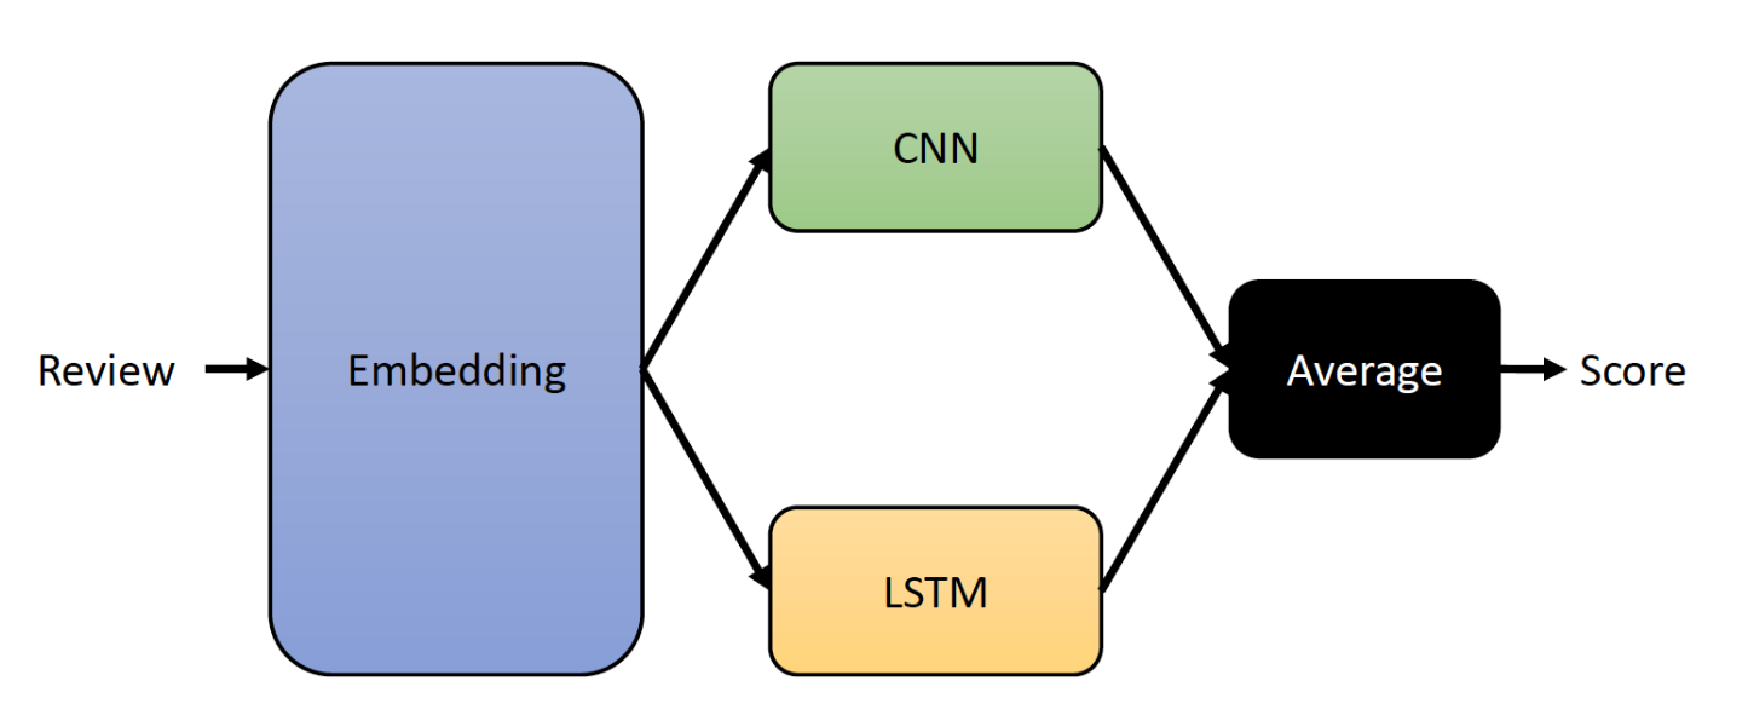
\includegraphics[width=1\linewidth]{images/chapter2/ensemble.pdf}
	\caption{Połączenie sieci konwolucyjnej i LSTM \cite{minaee2019deep}}
	\label{fig:ensemble}
\end{figure}
\chapter{Analiza i modelowanie}
W rozdziale tym opisane jest wykonane przez nas modelowanie. Wspieramy się tutaj wybranymi fragmentami kodu, natomiast cały kod dostępny jest w oddzielnym pliku. Wersje używanych bibliotek wylistowane są w Załączniku \ref{appendix} na końcu pracy inżynierskiej.

\section{Wstępne przygotowanie zbioru danych} 
W pierwszym etapie, nazwijmy wstępnym do tworzenia modeli, stworzyłyśmy notatnik w Google Colab zintegrowany z Dykiem Google i wczytałyśmy dane do \verb|DataFrame|'a.

\begin{lstlisting}[language=Python,frame=single, breaklines=true,caption=Wczytywanie surowych danych z Dysku Google do DataFrame'a.,label=code:readData]
import pandas as pd
from google.colab import drive
drive.mount('/content/drive')

data_file = "drive/MyDrive/IMDB_Dataset.csv"
data = pd.read_csv(data_file, header=0, low_memory=False)
\end{lstlisting}

\noindent Surowe dane przedstawione są na poniższym rysunku (Rysunek. \ref{fig:rawDataset}). \\ \\
\noindent Jak widać zbiór danych składa się z dwóch interesujących nas kolumn. Kolumna pierwsza o nazwie \textit{review} (dtype: object) zawiera surowe treści recenzji filmów wraz z tagami w języku HTML, natomiast kolumna druga o nazwie \textit{sentiment} zawiera informację, czy dana recenzja uznawana jest jako pozytywna czy negatywna --- etykieta (dtype: object). \\

%%%  ------------> obrazek
\begin{figure}[H]
	\centering
	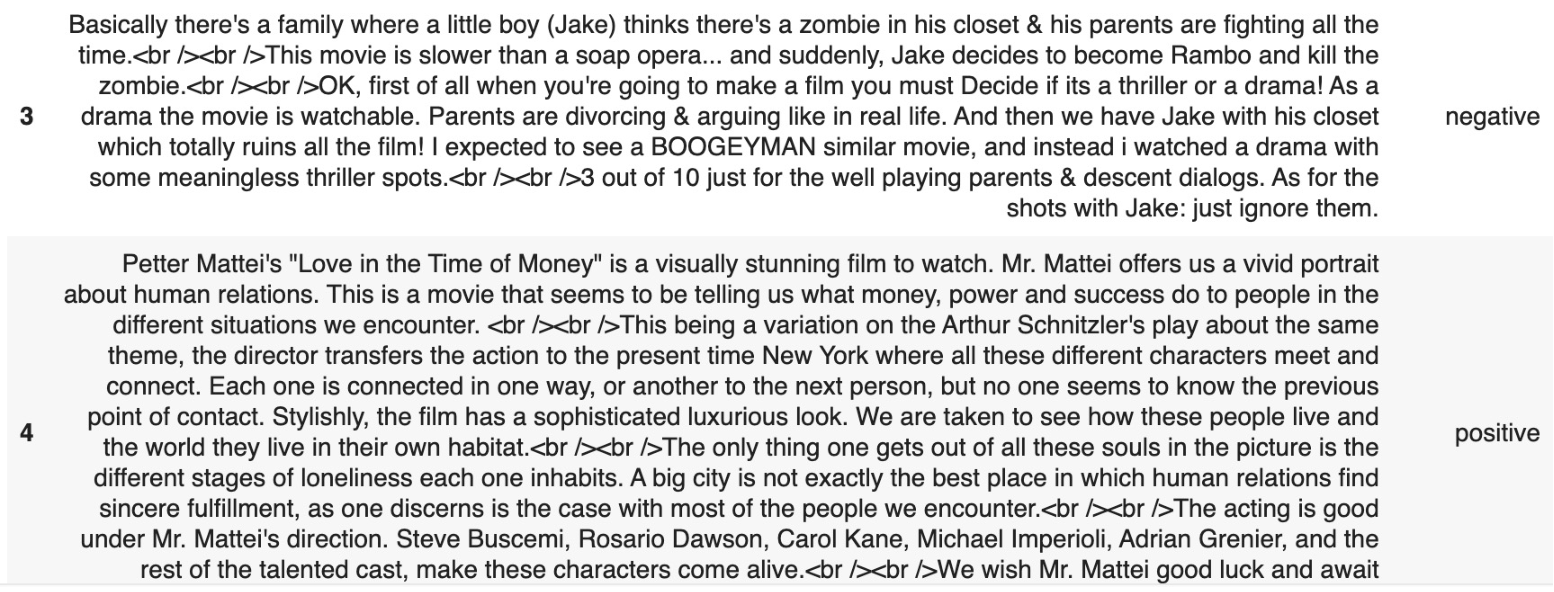
\includegraphics[width=0.95\linewidth]{images/chapter3/raw-data-example.pdf}
	\caption{Przykładowe próbki z surowego zbioru danych recenzji filmowych IMDB.}
	\label{fig:rawDataset}
\end{figure}


\noindent Jako że model matematyczny działa na wartościach liczbowych, kolumnę etykiet słownych zamieniłyśmy na etykiety w postaci liczb, gdzie etykieta 0 oznacza recenzję negatywną, a etykieta 1 pozytywną (zmiana dtype z object na int64). Na tym etapie usunęłyśmy również tagi HTML wykorzystując pakiet \verb|bs4|.


\begin{lstlisting}[language=Python,frame=single, breaklines=true, caption=Zmiana etykiet z typu obiekt na typ liczbowy.,label=code:labelChange]
labels = labels.replace("negative", 0)
labels = labels.replace("positive", 1)

from bs4 import BeautifulSoup
reviews = reviews.apply(lambda text: BeautifulSoup(text).get_text())
reviews.head()
\end{lstlisting}

%%%  ------------> obrazek
\begin{figure}[H]
	\centering
	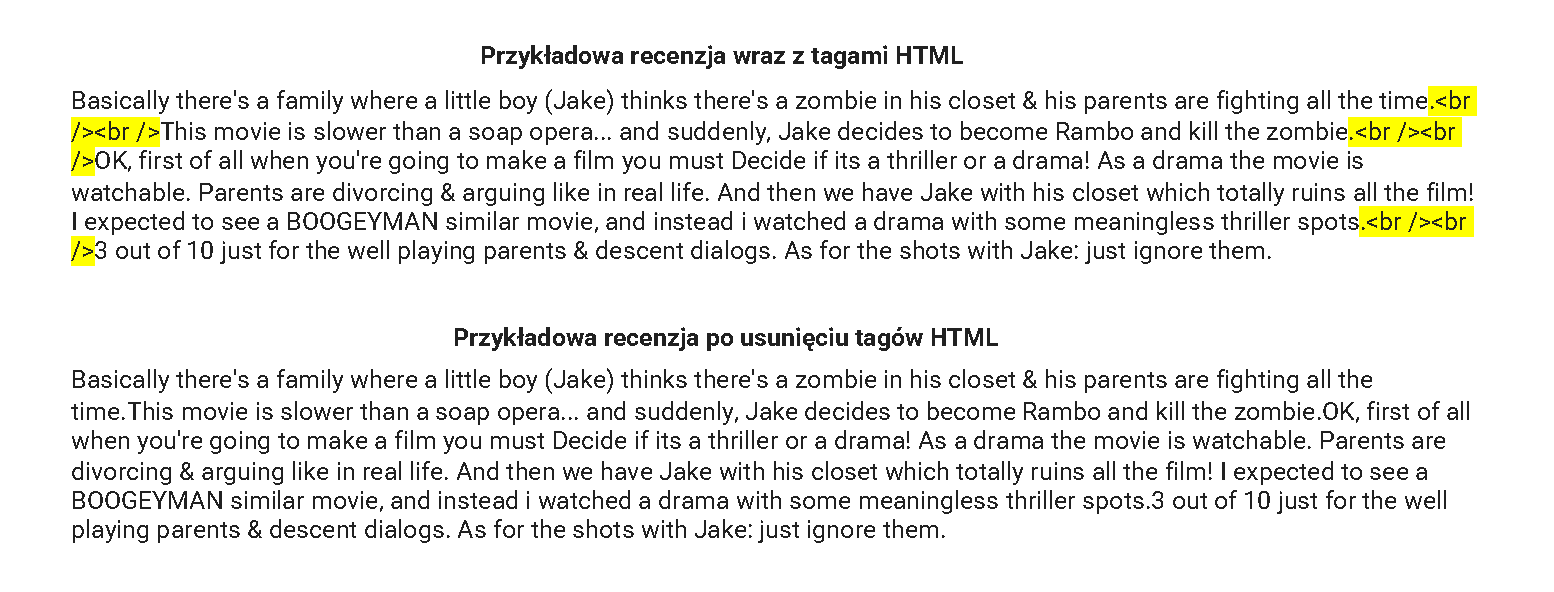
\includegraphics[width=0.95\linewidth]{images/chapter3/cleaned-data-example.pdf}
	\caption{Przykładowa recenzja przed usunięciem tagów HTML (surowa) oraz po usunięciu tagów.}
	\label{fig:cleaned}
\end{figure}

\noindent Przy okazji sprawdziłyśmy, czy zbiór jest dobrze zbalansowany --- czy liczba recenzji pozytywnych i negatywnych jest porównywalna. W kolejnym etapie podzieliłyśmy zbiór danych na dane treningowe i testowe w proporcji 80:20 używając metody \verb|train_test_split| z biblioteki \verb|Pandas| i ponownie sprawdziłyśmy, czy po wykonanym podziale nasze podzbiory są zbalansowane (train: 20 044 recenzje pozytywne i 19 956 recenzji negatywnych oraz test: 4 956 recenzji pozytywnych i 5 044 recenzje negatywne).

\begin{lstlisting}[language=Python,frame=single, breaklines=true, caption=Podział danych na zbiór treningowy i testowy.,label=code:split]
from sklearn.model_selection import train_test_split
train_data, test_data, train_labels, test_labels = train_test_split(reviews, labels, test_size=0.2, random_state=1)

train_labels = train_labels.astype('int')
test_labels = test_labels.astype('int')
\end{lstlisting}

\noindent Następnie bazując na wbudowanej liście angielskich słów stop-words rozbudowanej o znaki interpunkcyjne i kilka własnych znaków (głównie cudzysłowów), usunęłyśmy wyrazy popularnie występujące a więc i nic nie wnoszące, po czym dokonałyśmy prostej wektoryzacji używając klasy \verb|CountVectorizer|.

\begin{lstlisting}[language=Python,frame=single, breaklines=true, caption=Wektoryzacja zbiorów danych --- treningowego i testowego.,label=code:vectorization]
from sklearn.feature_extraction.text import CountVectorizer
count_vectorizer = CountVectorizer(stop_words=english_stopwords) 
train_data_count = count_vectorizer.fit_transform(train_data)
test_data_count = count_vectorizer.transform(test_data)
\end{lstlisting}



\section{Modelowanie}
Po wstępnym przygotowaniu danych przyszedł czas na modelowanie. Stworzyłyśmy 4 rodzaje modeli oraz dla każdego z nich wykonałyśmy optymalizacje hiperparametrów aby otrzymać jak najlepsze wyniki. W pierwszej kolejności stworzyłyśmy model wykorzystujący układ drzew decyzyjnych --- Las Losowy (\textit{Random Forest}).

\subsection{Las losowy}

Model klasyfikujący stworzyłyśmy używając klasy \verb|RandomForestClassifier| z pakietu \verb|sklearn.ensemble|. Dokładny opis tego algorytmu znajduje sie w rozdziale \ref{chapter:2} w sekcji \ref{sec:rf}.

\noindent Przy użyciu klasy \verb|Randomized| \verb|SearchCV| optymalizowałyśmy hiperparametry. Testowałyśmy działanie modelu dla różnych liczb estymatorów (n\_estimators)  wynoszących 10, 30 i 100, 300, 1000 oraz różnych głębokości drzew decyzyjnych (max\_depth) wynoszących 4, 8, 16, 32, 64, None (bez limitu głębości).

\begin{lstlisting}[language=Python,frame=single, breaklines=true, caption=Optymalizacja hiperparametrów RF (RandomizedSearchCV).,label=code:rf-hiper]
rf_params_count = {
	"n_estimators": [10, 30, 100, 300, 1000],
	"max_depth": [4, 8, 16, 32, 64, None]
}

rf_search_count = RandomizedSearchCV(RandomForestClassifier(), rf_params_count,refit= True, verbose= 3)
rf_search_count.fit(train_data_count, count)
rf_params_results_count = pd.DataFrame(rf_search_count.cv_results_)
rf_params_results_count.sort_values("rank_test_score").head(1)
\end{lstlisting}


\begin{table}
	\caption{Wyniki optymalizacji dla dwóch najlepszych iteracji --- z głębokością drzewa 16 i 64.}
	\begin{center}
		\begin{tabular}{c  c  || c || c || c  c  c  c  c  || c  || c }
			\hline
			$\overline{t_{fit}}$&$\overline{t_{sc}}$ &\textbf{N} & \textbf{D}	& sc$_1$&	sc$_2$ &sc$_3$ &	sc$_4$ &	sc$_5$	& \textbf{$\overline{sc}$ }&	$\pm$	\\
			\hline
			685.14	&	0.05	&	\textbf{1000}& \textbf{64}	&	0.874	& 0.870 &	0.866&	0.88 &	0.869 &	\textbf{0.869}&	0.003 \\
			103.46& 		0.05 &		\textbf{1000}	& \textbf{16}	& 0.859 &	0.855 &	0.854 &	0.854 &	0.868& 	\textbf{0.856}& 0.002 \\
			\hline
		\end{tabular} \\
		{\scriptsize 	sc --- score, t --- time (s), N --- n\_estimators, D --- max\_depth}
	\end{center}
\end{table}


\noindent Jak widać najlepszy wynik (0.87) został otrzymany dla liczby estymatorów równej 1000 oraz głębokości drzewa równej 64. Jednakże wynik otrzymany przy użyciu 4$\times$ mniejszej głębokości (16) był niewiele niższy (0.86), a średni czas trenowanie prawie 7$\times$ krótszy --- jedynie 103.5 s w porównaniu do 685s. Widząc takie rezultaty, należy się zastanowić czy użycie drzew o mniejszej maksymalnej głębokości nie jest korzystniejsze. Trzeba pamiętać o tym, że drzewa decyzyjne mają tendencje do nadmiernego dopasowywania się do danych treningowych, a im głębsze drzewa tym o to przeuczenie łatwiej.


\begin{lstlisting}[language=Python,frame=single, breaklines=true, caption=Trenowanie modelu lasu losowego dla 1000 estymatorów i głębokości 64.,label=code:rf-train]
random_forest_count = RandomForestClassifier(n_estimators = 1000, max_depth=64, verbose=True)
random_forest_count.fit(train_data_count, train_labels)
\end{lstlisting}

\begin{Verbatim}
RandomForestClassifier(
			bootstrap=True,
			ccp_alpha=0.0,
			class_weight=None,
			criterion='gini',
			max_depth=64,
			max_features='auto',
			max_leaf_nodes=None,
			max_samples=None,
			min_impurity_decrease=0.0,
			min_impurity_split=None,
			min_samples_leaf=1,
			min_samples_split=2,
			min_weight_fraction_leaf=0.0,
			n_estimators=1000,
			n_jobs=None,
			oob_score=False,
			random_state=None,
			verbose=True,
			warm_start=False
			)
\end{Verbatim}


\noindent Trenowanie zajęło 13. 8 minuty. Następnie przy użyciu wytrenowanego modelu wykonałysmy predykcję.


\begin{lstlisting}[language=Python,frame=single, breaklines=true, caption=Predykcja z użyciem wytrenowanego modelu lasu losowego.,label=code:rf-pred]
random_forest_predictions_count = random_forest_count.predict(test_data_count)
\end{lstlisting}


%%%  ------------> obrazek
\begin{figure}[H]
	\centering
	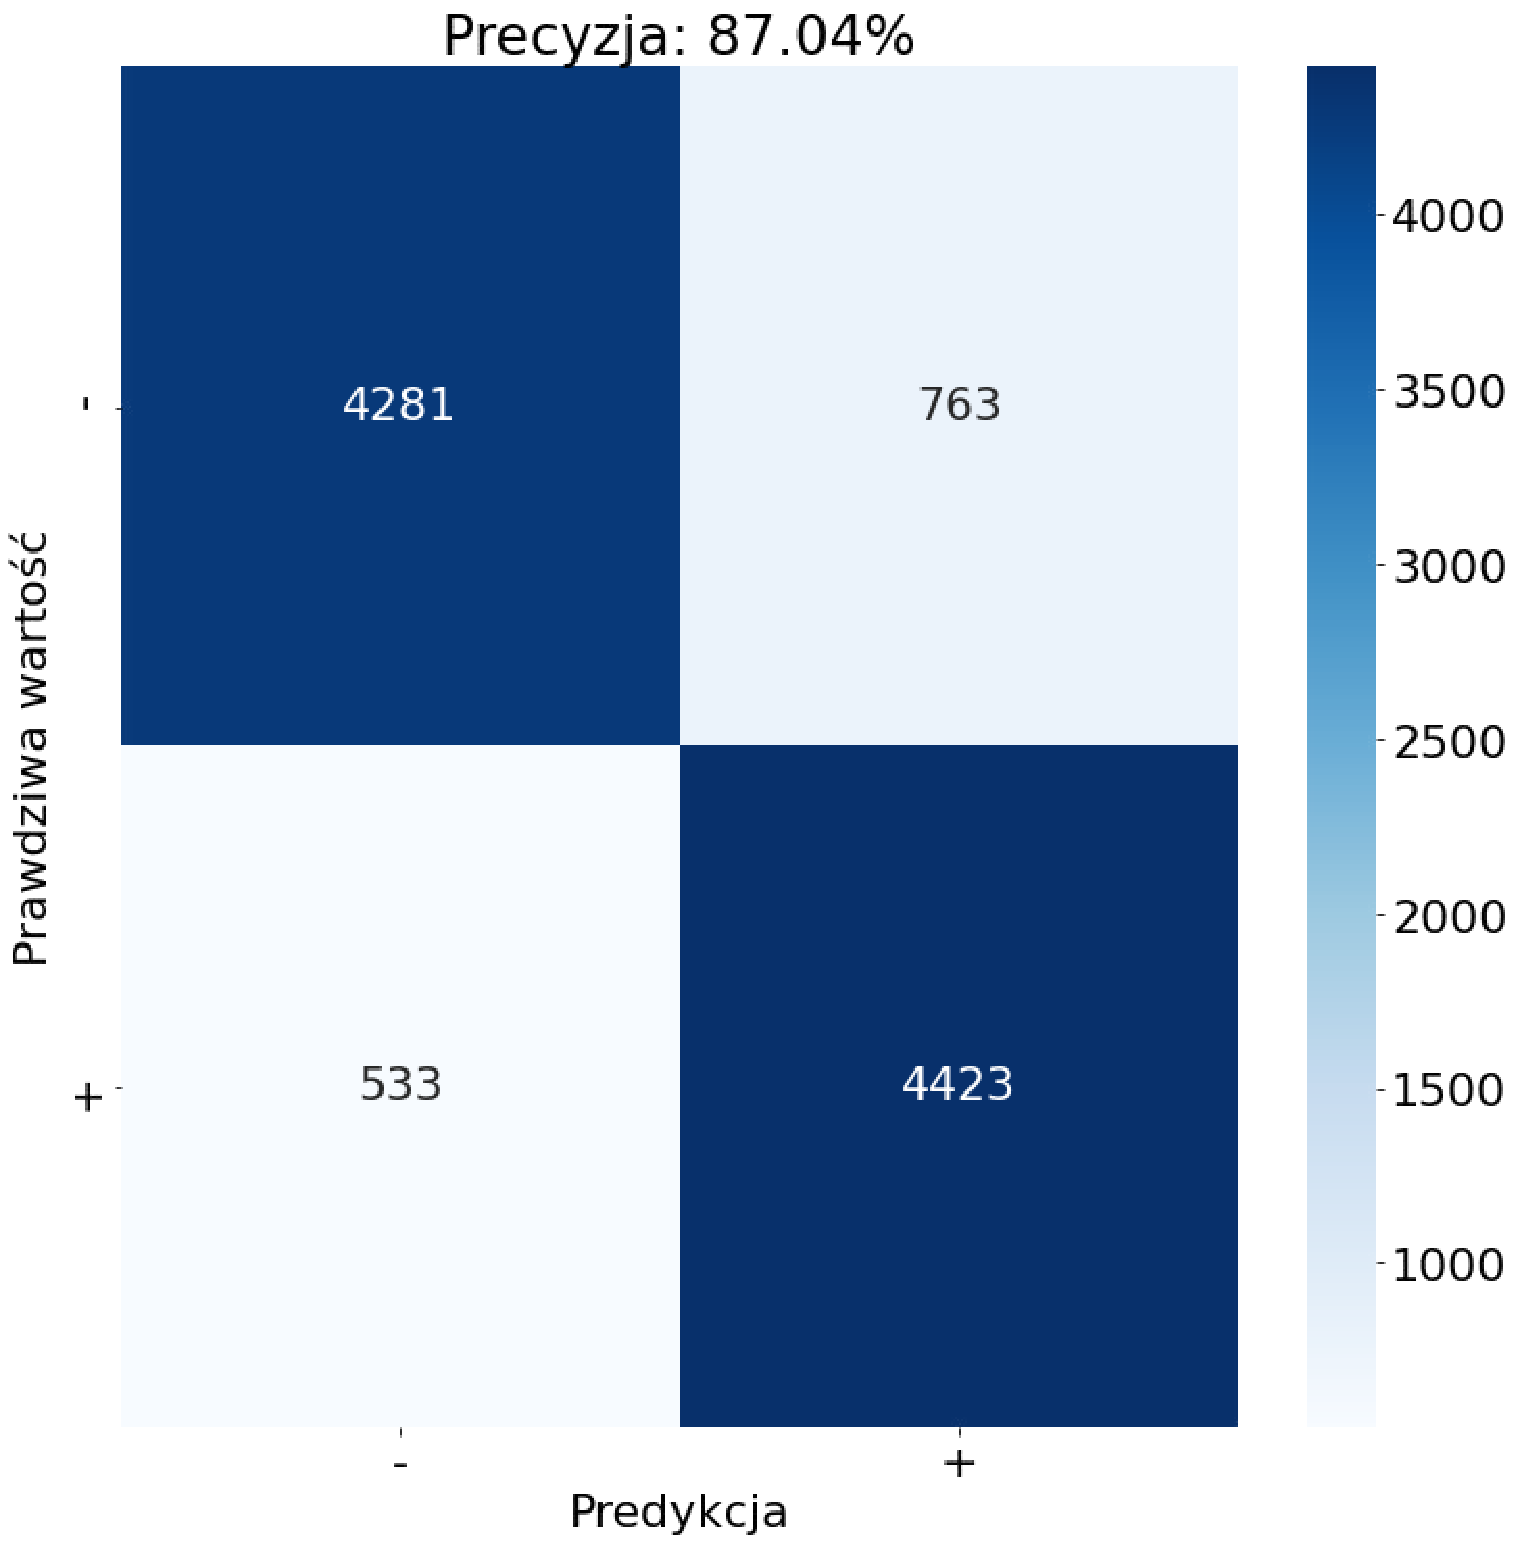
\includegraphics[width=0.5\linewidth]{images/chapter3/rf-macierz.pdf}
	\caption{Wyniki klasyfikacji z użyciem lasu losowego dla n\_estimators=1000 i max\_depth=64. Trening modelu zajął 13.8 minuty.}
	\label{fig:macierz-rf}
\end{figure}

\noindent Kolorem granatowym zostały oznaczone wartości przewidziane prawidłowo przez skonstruowany przez nas model --- 4423 wartości zostały zaklasyfikowane prawidłowo jako pozytywne i 4281 wartości zostały zaklasyfikowane prawidłowo jako negatywne, co po zsumowaniu daje 8704 prawidłowo sklasyfikowane wartości na 10~000 przykładów. Tak więc precyzja predykcji wynosi 87.04\%. Ponadto 763 przykładów zostało błędnie sklasyfikowanych jako pozytywne i 533 błędnie jako negatywne (ćwiartki w kolorze błękitnym). Całkowity czas trenowania modelu zajął tutaj prawie 14 minut. Wydaje się nam, że jest to dosyć długi czas jak na stosunkowo mały (40~000 przykładów) zbiór treningowy.

\noindent W związku z tym, dla porównania wykonałyśmy również analogiczne modelowanie (fitowanie) dla maksymalnej głębokości drzew wynoszącej 32. Czas uległ znacznemu skróceniu. Trenowanie tego samego zbioru zajęło niecałe 4 minuty, a osiągnięta precyzja wyniosła 86.65\%, a więc była tylko o 0.39\% mniejsza niż dla 2$\times$ głębszych drzew. Szczegółowe wyniki przedstawione są w załączonym notatniku Google Colab. Wynik ten wyraźnie sugeruje, że należy się zawsze zastanowić nad sensem dużej głębokości drzew, gdyż w płytszymi drzewami również można osiągnąć zadowalające wyniki, a przy tym znacznie zredukować czas wykonywanych obliczeń.

\noindent Przy pomocy zaimplementowanej przez nas dedykowanej metody (Listing. \ref{code:rf-prior}) został też wyznaczony priorytet cech (\textit{feature importance}), na bazie których następowały podziały w kolejnych węzłach drzew decyzyjnych.

\begin{lstlisting}[language=Python,frame=single, breaklines=true, caption=Metoda do wyznaczania i wizualizacji priorytetu cech dla drzewa decyzyjnego.,label=code:rf-prior]
def plot_feature_importance(model, vectorizer):
	feature_importance = np.array(model.feature_importances_)
	feature_names = np.array(vectorizer.get_feature_names())
	data = pd.DataFrame({'feature_names': feature_names, 'feature_importance': feature_importance})
	
	max_data = data.nlargest(20, ['feature_importance'])
	
	max_data.plot(kind='barh', x='feature_names', y='feature_importance', color=blue_0)
	plt.show()

plot_feature_importance(random_forest_count, count_vectorizer)
\end{lstlisting}


%%%  ------------> obrazek
\begin{figure}[H]
	\centering
	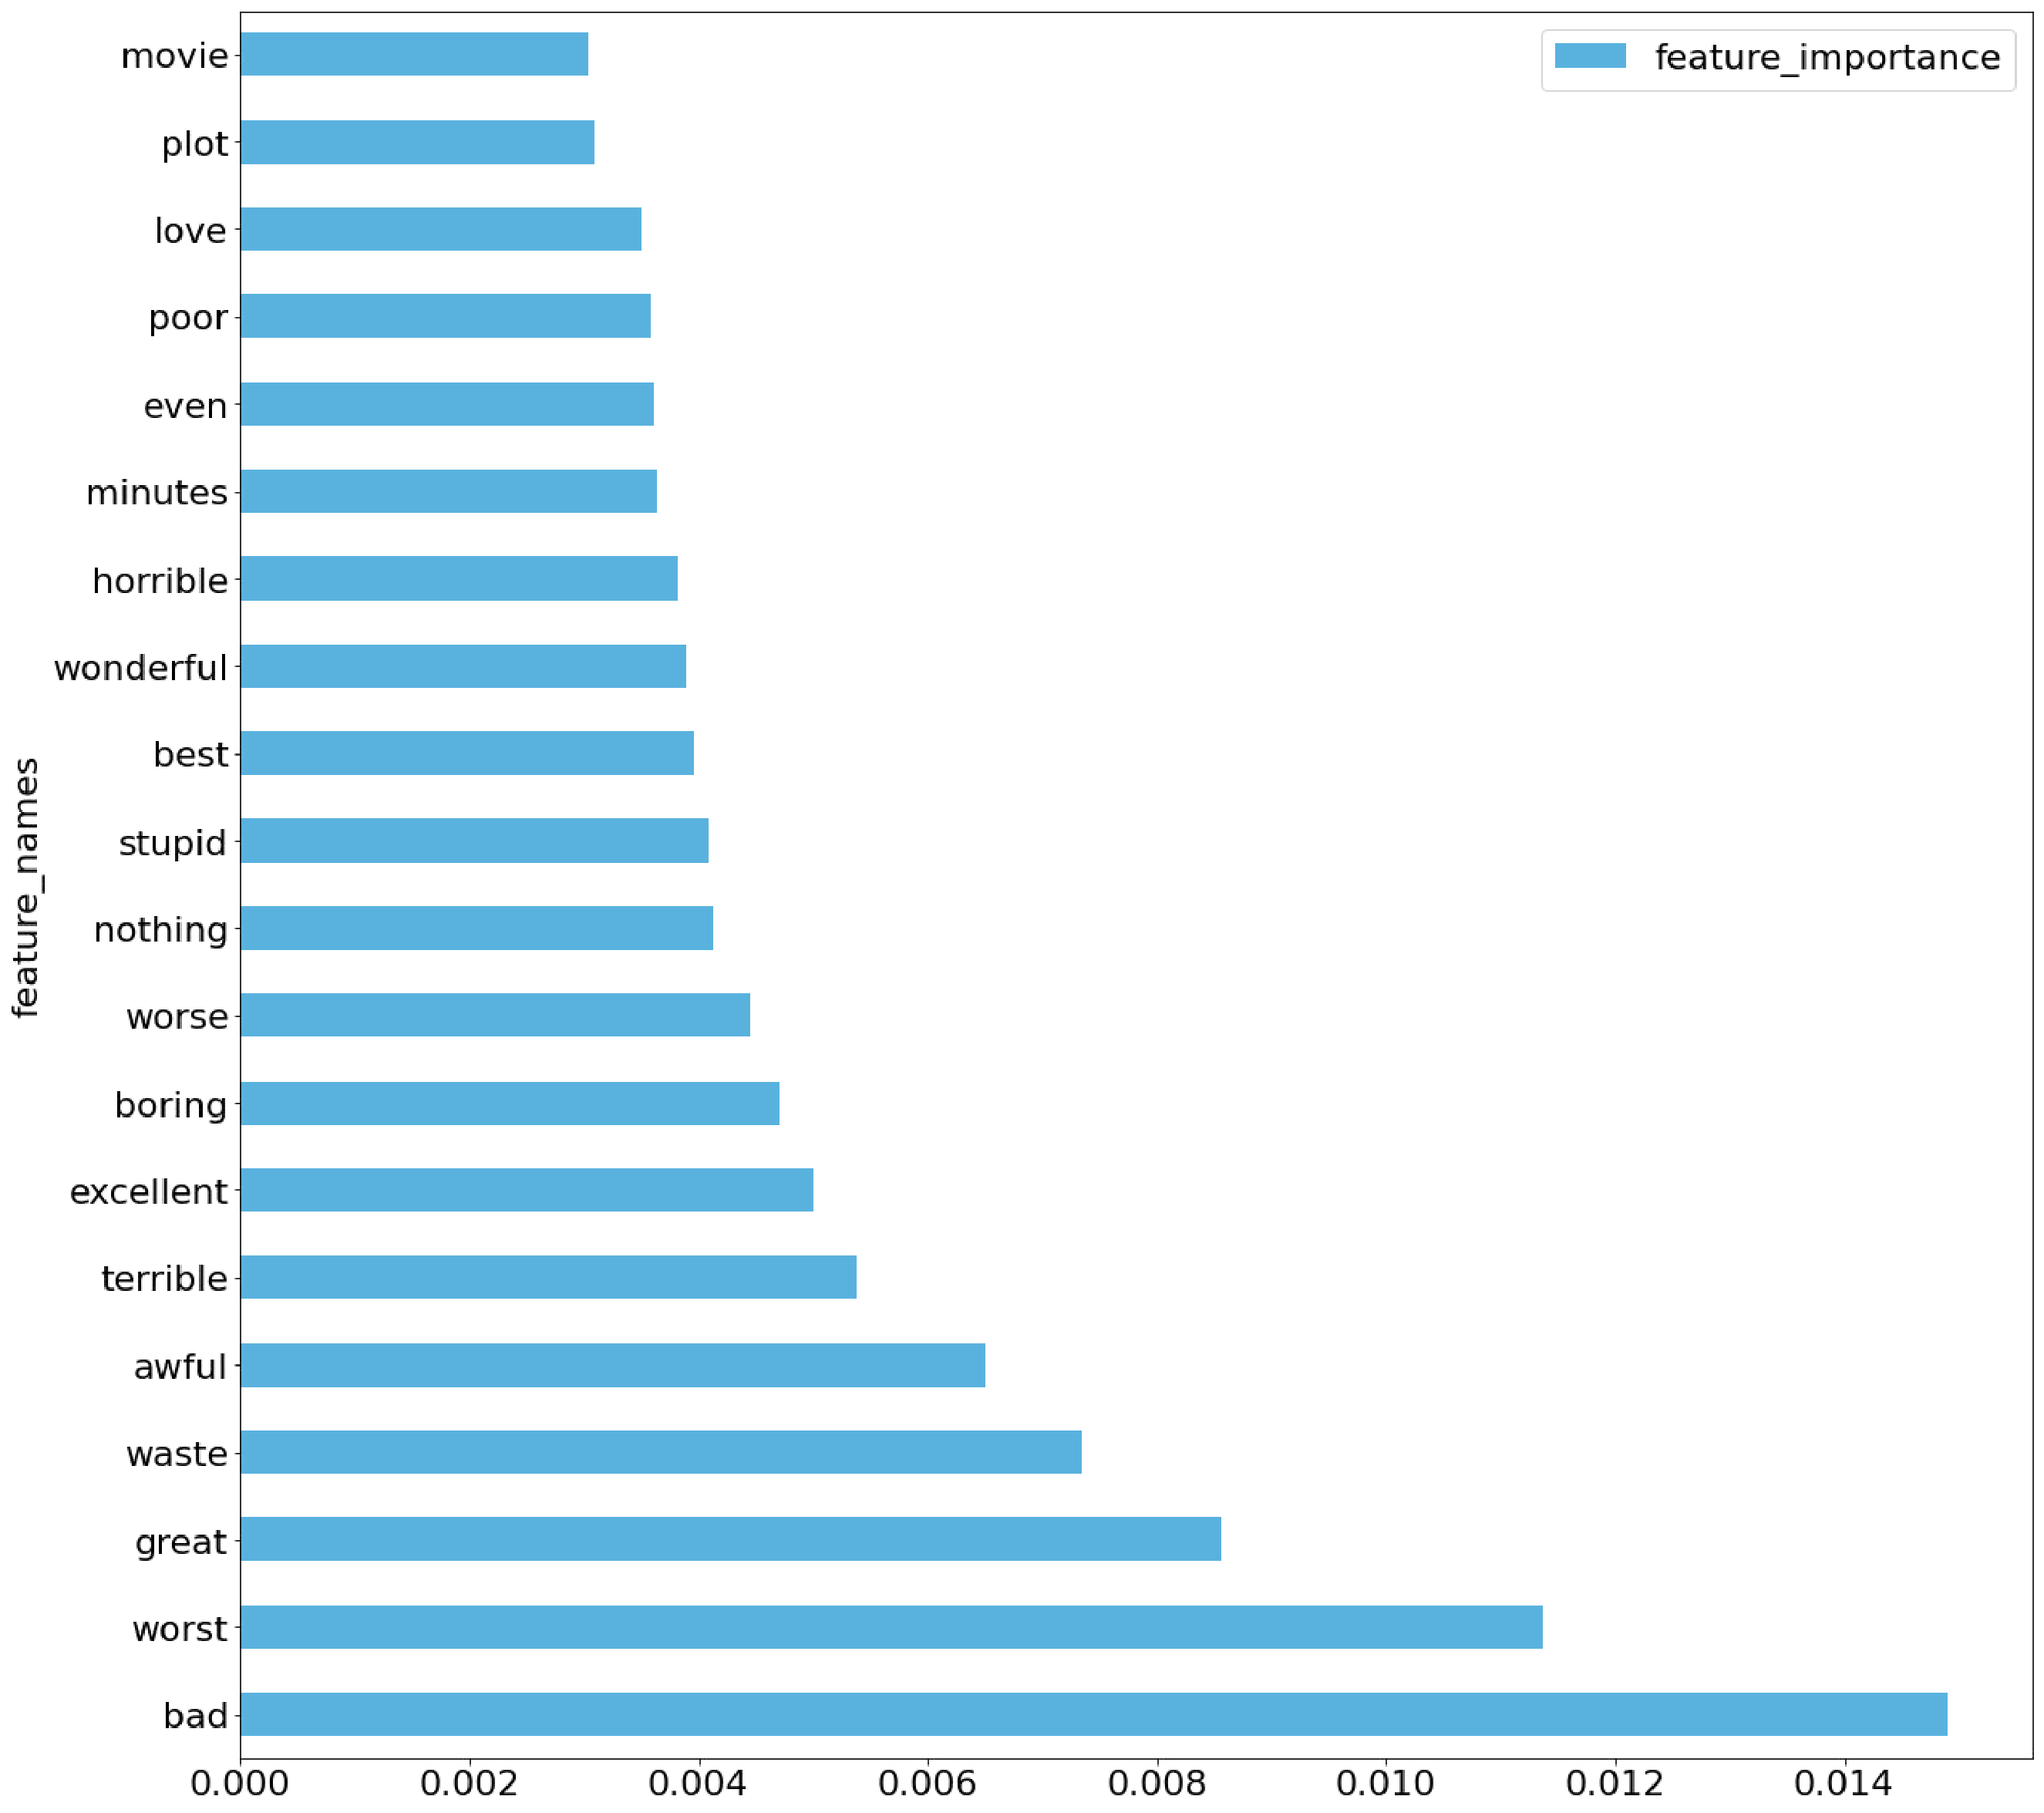
\includegraphics[width=0.55\linewidth]{images/chapter3/rf-feature-import.pdf}
	\caption{Ważność cech w drzewach decyzyjnych.}
	\label{fig:rf-fi}
\end{figure}

\noindent Znalazłysmy też ciekawe narzędzie --- bibliotekę \verb|LIME| --- które umożliwia zwizualizowanie wydźwięków kluczowych słów, które posłużyły do sklasyfikowania danej recenzji jako pozytywnej lub negatywnej. Poszczególne słowa są w tym przypadku oznaczone albo kolorem pomarańczowym (jeżeli są pozytywne) albo niebieskim (gdy są negatywne). Intensywność koloru mówi o tym jak bardzo jwydźwięk ten jest pozytywny lub negatywny. Na poniższym rysunku (Rysunek. \ref{fig:rf-lime}) znajduję się wizualizacja dla przykładowej recenzji pozytywnej (góra) oraz negatywnej (dół).

%%%  ------------> obrazek
\begin{figure}[H]
	\centering
	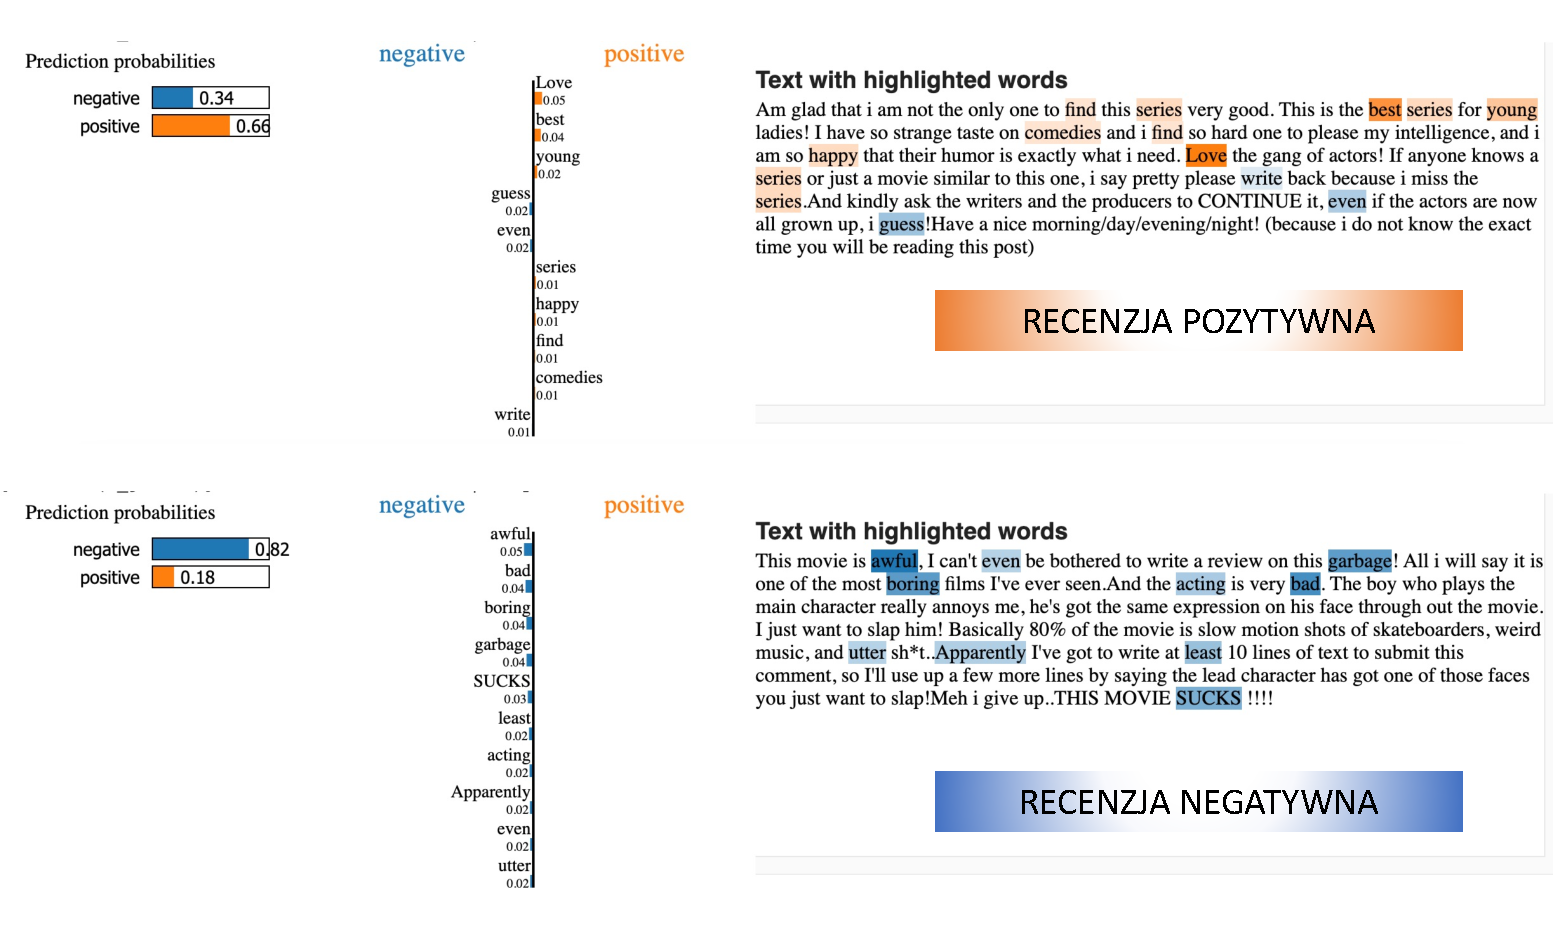
\includegraphics[width=0.8\linewidth]{images/chapter3/rf-lime.pdf}
	\caption{Wykres LIME wydźwięków kluczowych słów dla przykładowej recenzji pozytywnej (góra) oraz negatywnej (dół).}
	\label{fig:rf-lime}
\end{figure}

\noindent Istnieje również możliwość wykonania wizualizacji drzew decyzyjnych, co w prostu sposób pozwala interpretować i wyciągać wnioski. Jednakże głębokość naszych drzew uniemożliwia przedstawienie ich w sposób czytelny, dlatego wizualizacja została pominięta.

\subsection{SVM}
Kolejny model klasyfikacyjny stworzyłyśmy używając klasy \verb|LinearSVC| z pakietu \verb|sklearn.svm|. Dodatkowo przy użyciu klasy \verb|RandomizedSearchCV| oraz  \verb|GridSearchCV| szukałyśmy optymalnego parametru 'C'. Parametr 'C' informuje o tym, jak bardzo chce się uniknąć błędnej klasyfikacji każdego przykładu ze zbioru treningowego \cite{paramC}. Dla dużych wartości 'C' optymalizator wybiera hiperpłaszczyznę o mniejszym marginesie, jeśli ta hiperpłaszczyzna lepiej radzi sobie z prawidłowym sklasyfikowaniem wszystkich punktów treningowych. Przeciwnie, bardzo mała wartość 'C' spowoduje, że optymalizator będzie szukał hiperpłaszczyzny oddzielającej o większym marginesie, nawet jeśli ta hiperpłaszczyzna błędnie zaklasyfikuje większą liczbę punktów (Rysunek. \ref{fig:param-C}). Parametr 'C' jest zasadniczo parametrem regularyzacji, który kontroluje kompromis między osiągnięciem małego błędu dopasowania modelu na danych uczących a minimalizacją norm wag w równaniu modelu.

%%%  ------------> obrazek
\begin{figure}[H]
	\centering
	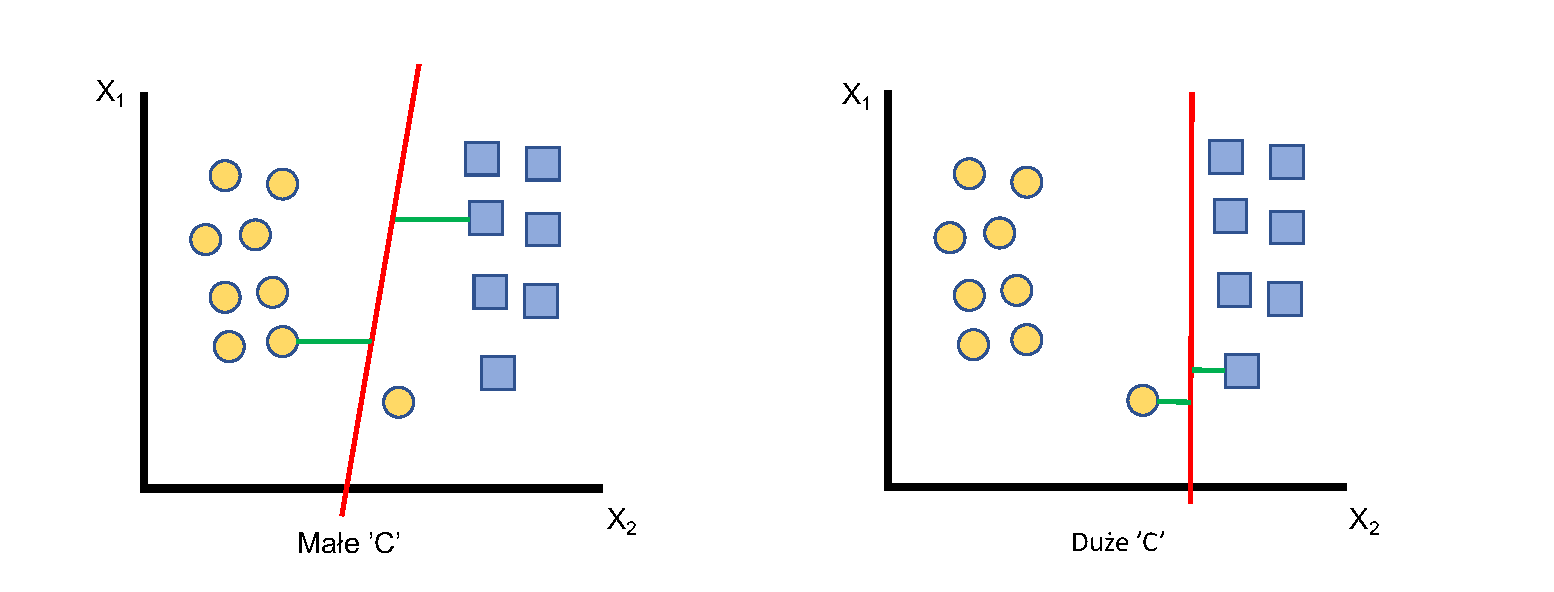
\includegraphics[width=0.85\linewidth]{images/chapter3/param-C.pdf}
	\caption{Idea obrazująca parametr 'C' --- płaszczyzny dla małej (lewy) i dużej (prawy) wartości parametru 'C'.}
	\label{fig:param-C}
\end{figure}


\noindent Pierwsza optymalizacja została wykonana z użyciem klasy \verb|RandomizedSearchCV| dla: \verb|params = {'C': scipy.stats.expon(scale=10)}|.


\begin{lstlisting}[language=Python,frame=single, breaklines=true, caption=Optymalizacja hiperparametrów SVM (RandomizedSearchCV).,label=code:svm]
from sklearn.svm import LinearSVC
import scipy
from sklearn.model_selection import RandomizedSearchCV

params = {'C': scipy.stats.expon(scale=10)}

grid_count2 = RandomizedSearchCV(LinearSVC(max_iter=5000), params, refit= True, verbose= 3)
grid_count2.fit(train_data_count, train_labels)
param_results = pd.DataFrame(grid_count2.cv_results_)
param_results.sort_values("rank_test_score").head(1)
\end{lstlisting}

\bigskip
\begin{table} [H]
	\caption{Wyniki optymalizacji dla najlepszych iteracji RandomizedSearchCV.}
	\begin{center}
		\begin{tabular}{c  c || c || c  c  c  c  c  || c  || c }
			\hline
			$\overline{t_{fit}}$&$\overline{t_{sc}}$ &\textbf{C} &	sc$_1$&	sc$_2$ &sc$_3$ &	sc$_4$ &	sc$_5$	& \textbf{$\overline{sc}$ }&	$\pm$	\\
			\hline
			10.9&	0.005  & \textbf{0.533} & 0.865 &	0.865 &	0.868 &	0.863 &	0.867 &	\textbf{0.866} &	0.002 \\
			18.2&	0.005&	\textbf{2.29}&	0.861 &	0.862 &	0.864 &	0.856&	0.861&	\textbf{0.861}&	0.002 \\
			\hline
		\end{tabular} \\
		{\scriptsize sc --- score, t --- time (s)}
	\end{center}
\end{table}

\noindent Ze względu na to, że model osiągał znacząco lepsze wyniki z niskimi wartościami parametru 'C', zdecydowałyśmy się na dalszą optymalizację --- tym razem przy użyciu \verb|GridSearchCV| dla: \verb|params = {'C': np.linspace(0, 1, num=1000)}|.

\begin{lstlisting}[language=Python,frame=single, breaklines=true, caption=Optymalizacja hiperparametrów SVM (GridSearchCV).,label=code:svm1]
from sklearn.svm import LinearSVC
import scipy
from sklearn.model_selection import GridSearchCV

params = {'C': np.linspace(0, 1, num=1000)}

grid_count2 = GridSearchCV(LinearSVC(max_iter=500),  params, verbose= 3)
grid_count2.fit(train_data_count, train_labels)
param_results = pd.DataFrame(grid_count2.cv_results_)
param_results.sort_values('rank_test_score').head(1)
\end{lstlisting}

\bigskip
\begin{table} [H]
	\caption{Wyniki optymalizacji dla najlepszych iteracji GridSearchCV.}
	\begin{center}
		\begin{tabular}{c  c || c || c  c  c  c  c  || c  || c }
			\hline
			$\overline{t_{fit}}$&$\overline{t_{sc}}$ &\textbf{C} &	sc$_1$&	sc$_2$ &sc$_3$ &	sc$_4$ &	sc$_5$	& \textbf{$\overline{sc}$ }&	$\pm$	\\
			\hline
			0.44&	0.006&	\textbf{0.003}&	0.889 &	0.895 &	0.894 &	0.889&	0.891&	\textbf{0.891}&	0.002 \\
			0.49&	0.006&	\textbf{0.004}&	0.889 &	0.894 &	0.894 &	0.889&	0.891&	\textbf{0.891}&	0.002 \\
			\hline
		\end{tabular} \\
		{\scriptsize sc --- score, t --- time (s)}
	\end{center}
\end{table}

\noindent Jak widać, najlepsze wyniki otrzymałyśmy dla parametru 'C', który wynosi $\approx$0.003, a dokładnie 0.00300300300\\3003003, w związku z czym zecydowałyśmy się go użyć w dalszym modelowaniu.
Poniżej znajdują się fragmenty kodu odpowiadające trenowaniu (fitowaniu) modelu \verb|LinearSVC| (Listing. \ref{code:svc-train}) oraz predykcji wartości wyjścia (Listing. \ref{code:svc-pred}).

\bigskip

\begin{lstlisting}[language=Python,frame=single, breaklines=true, caption=Trening SVM dla C 0.003003003003003003.,label=code:svc-train]
svc_classifier_count = LinearSVC(max_iter=500, C=0.003003003003003003)
svc_classifier_count.fit(train_data_count, train_labels)
\end{lstlisting}

\bigskip
\begin{Verbatim}
LinearSVC(
	C=0.003003003003003003,
	class_weight=None,
	dual=True,
	fit_intercept=True, 
	intercept_scaling=1,
	loss='squared_hinge', 
	max_iter=500, 
	multi_class='ovr', 
	penalty='l2', 
	random_state=None, 
	tol=0.0001, 
	verbose=0
	)
\end{Verbatim}

\bigskip
\begin{lstlisting}[language=Python,frame=single, breaklines=true, caption=Predykcja SVM dla C 0.003003003003003003.,label=code:svc-pred]
svc_predictions_count = svc_classifier_count.predict(test_data_count)
print_metrics(svc_predictions_count)
\end{lstlisting}

\noindent Na rysunku (Rysunek. \ref{fig:macierz-svc}) przedstawiona jest macierz omyłek (pomyłek) zestawiająca wartości prawdziwe oraz te otrzymane w wyniku predykcji wraz z zależnościami pomiędzy nimi.

%%%  ------------> obrazek
\begin{figure}[H]
	\centering
	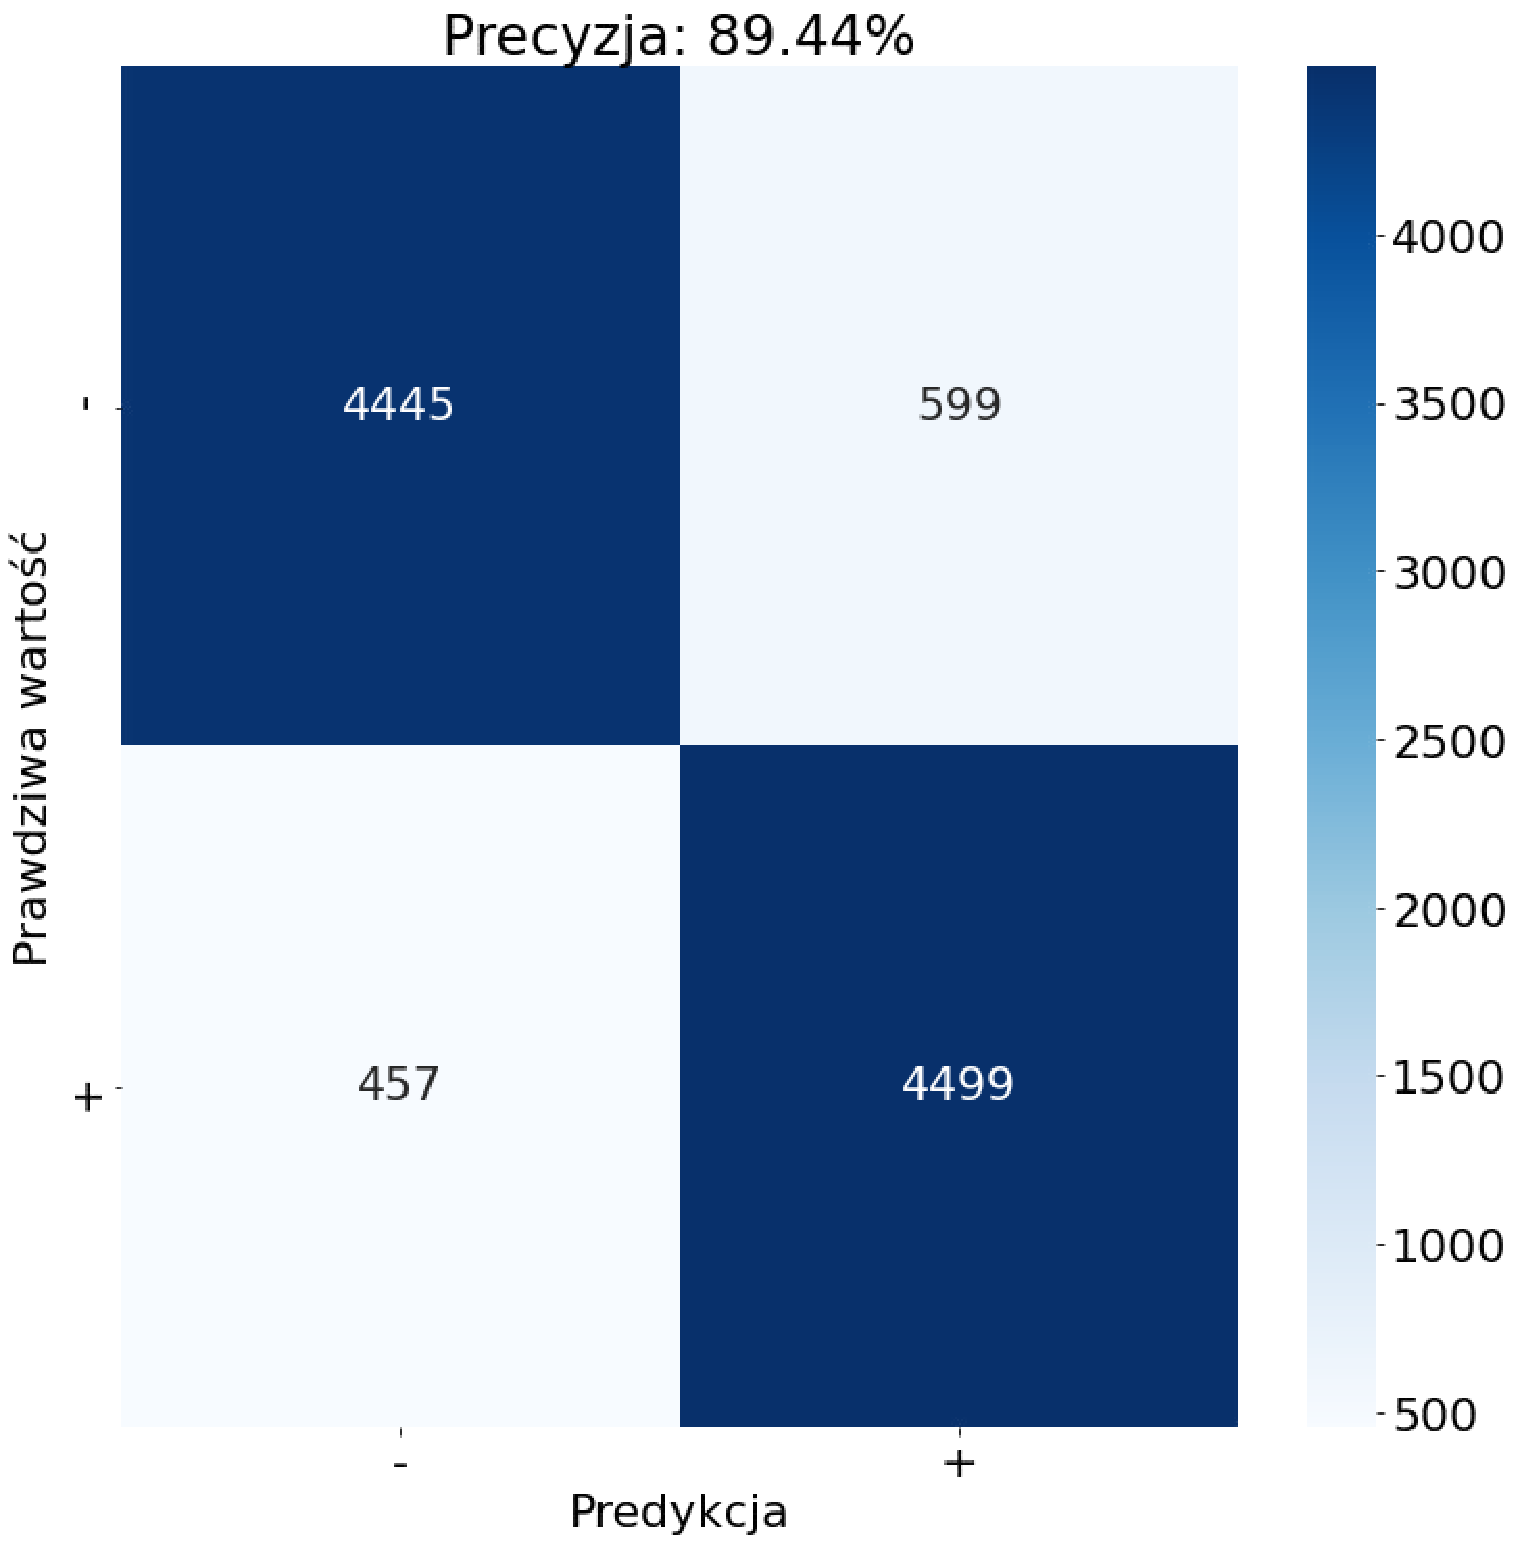
\includegraphics[width=0.5\linewidth]{images/chapter3/svc-macierz.pdf}
	\caption{Wyniki klasyfikacji z użyciem maszyny wektorów nośnych dla parametru C $\approx$ 0.003.}
	\label{fig:macierz-svc}
\end{figure}

\noindent Kolorem granatowym zostały oznaczone wartości przewidziane prawidłowo przez skonstruowany przez nas model --- 4499 wartości zostały zaklasyfikowane prawidłowo jako pozytywne i 4445 wartości zostały zaklasyfikowane prawidłowo jako negatywne, co po zsumowaniu daje 8944 prawidłowo sklasyfikowane wartości na 10~000 przykładów. Tak więc precyzja predykcji wynosi 89.44\%. Wynik wydaje się być logiczny. Ponadto 599 przykładów zostało błędnie sklasyfikowanych jako pozytywne i 457 błędnie jako negatywne (ćwiartki w kolorze błękitnym).

\noindent Na poniższym listingu (Listing. \ref{code:svc-visual}) przedstawiona jest implementacja metody \verb|plot_| \verb|coefficients(...)|, która umożliwia wykonanie wizualizacji najistotniejszych słów po klasyfikacji, które mają wydźwięk negatywny (kolor niebieski) lub pozytywny (kolor różowy).

\begin{lstlisting}[language=Python,frame=single, breaklines=true, caption=Wizualizacja SVM.,label=code:svc-visual]
from sklearn.feature_extraction.text import CountVectorizer
from sklearn.svm import LinearSVC
import matplotlib.pyplot as plt

def plot_coefficients(classifier, feature_names, top_features=20):
	coef = classifier.coef_.ravel()
	top_positive_coefficients = np.argsort(coef)[-top_features:]
	top_negative_coefficients = np.argsort(coef)[:top_features]
	top_coefficients = np.hstack([top_negative_coefficients, top_positive_coefficients])
	
	
	# create plot
	plt.figure(figsize=(15, 5))
	colors = [blue_0 if c < 0 else pink_0 for c in coef[top_coefficients]]
	plt.bar(np.arange(2 * top_features), coef[top_coefficients], color=colors)
	feature_names = np.array(feature_names)
	plt.xticks(np.arange(1, 1 + 2 * top_features), feature_names[top_coefficients], rotation=60, ha='right')
	plt.show()

plot_coefficients(svc_classifier_count, count_vectorizer.get_feature_names())	
\end{lstlisting}

%%%  ------------> obrazek
\begin{figure}[H]
	\centering
	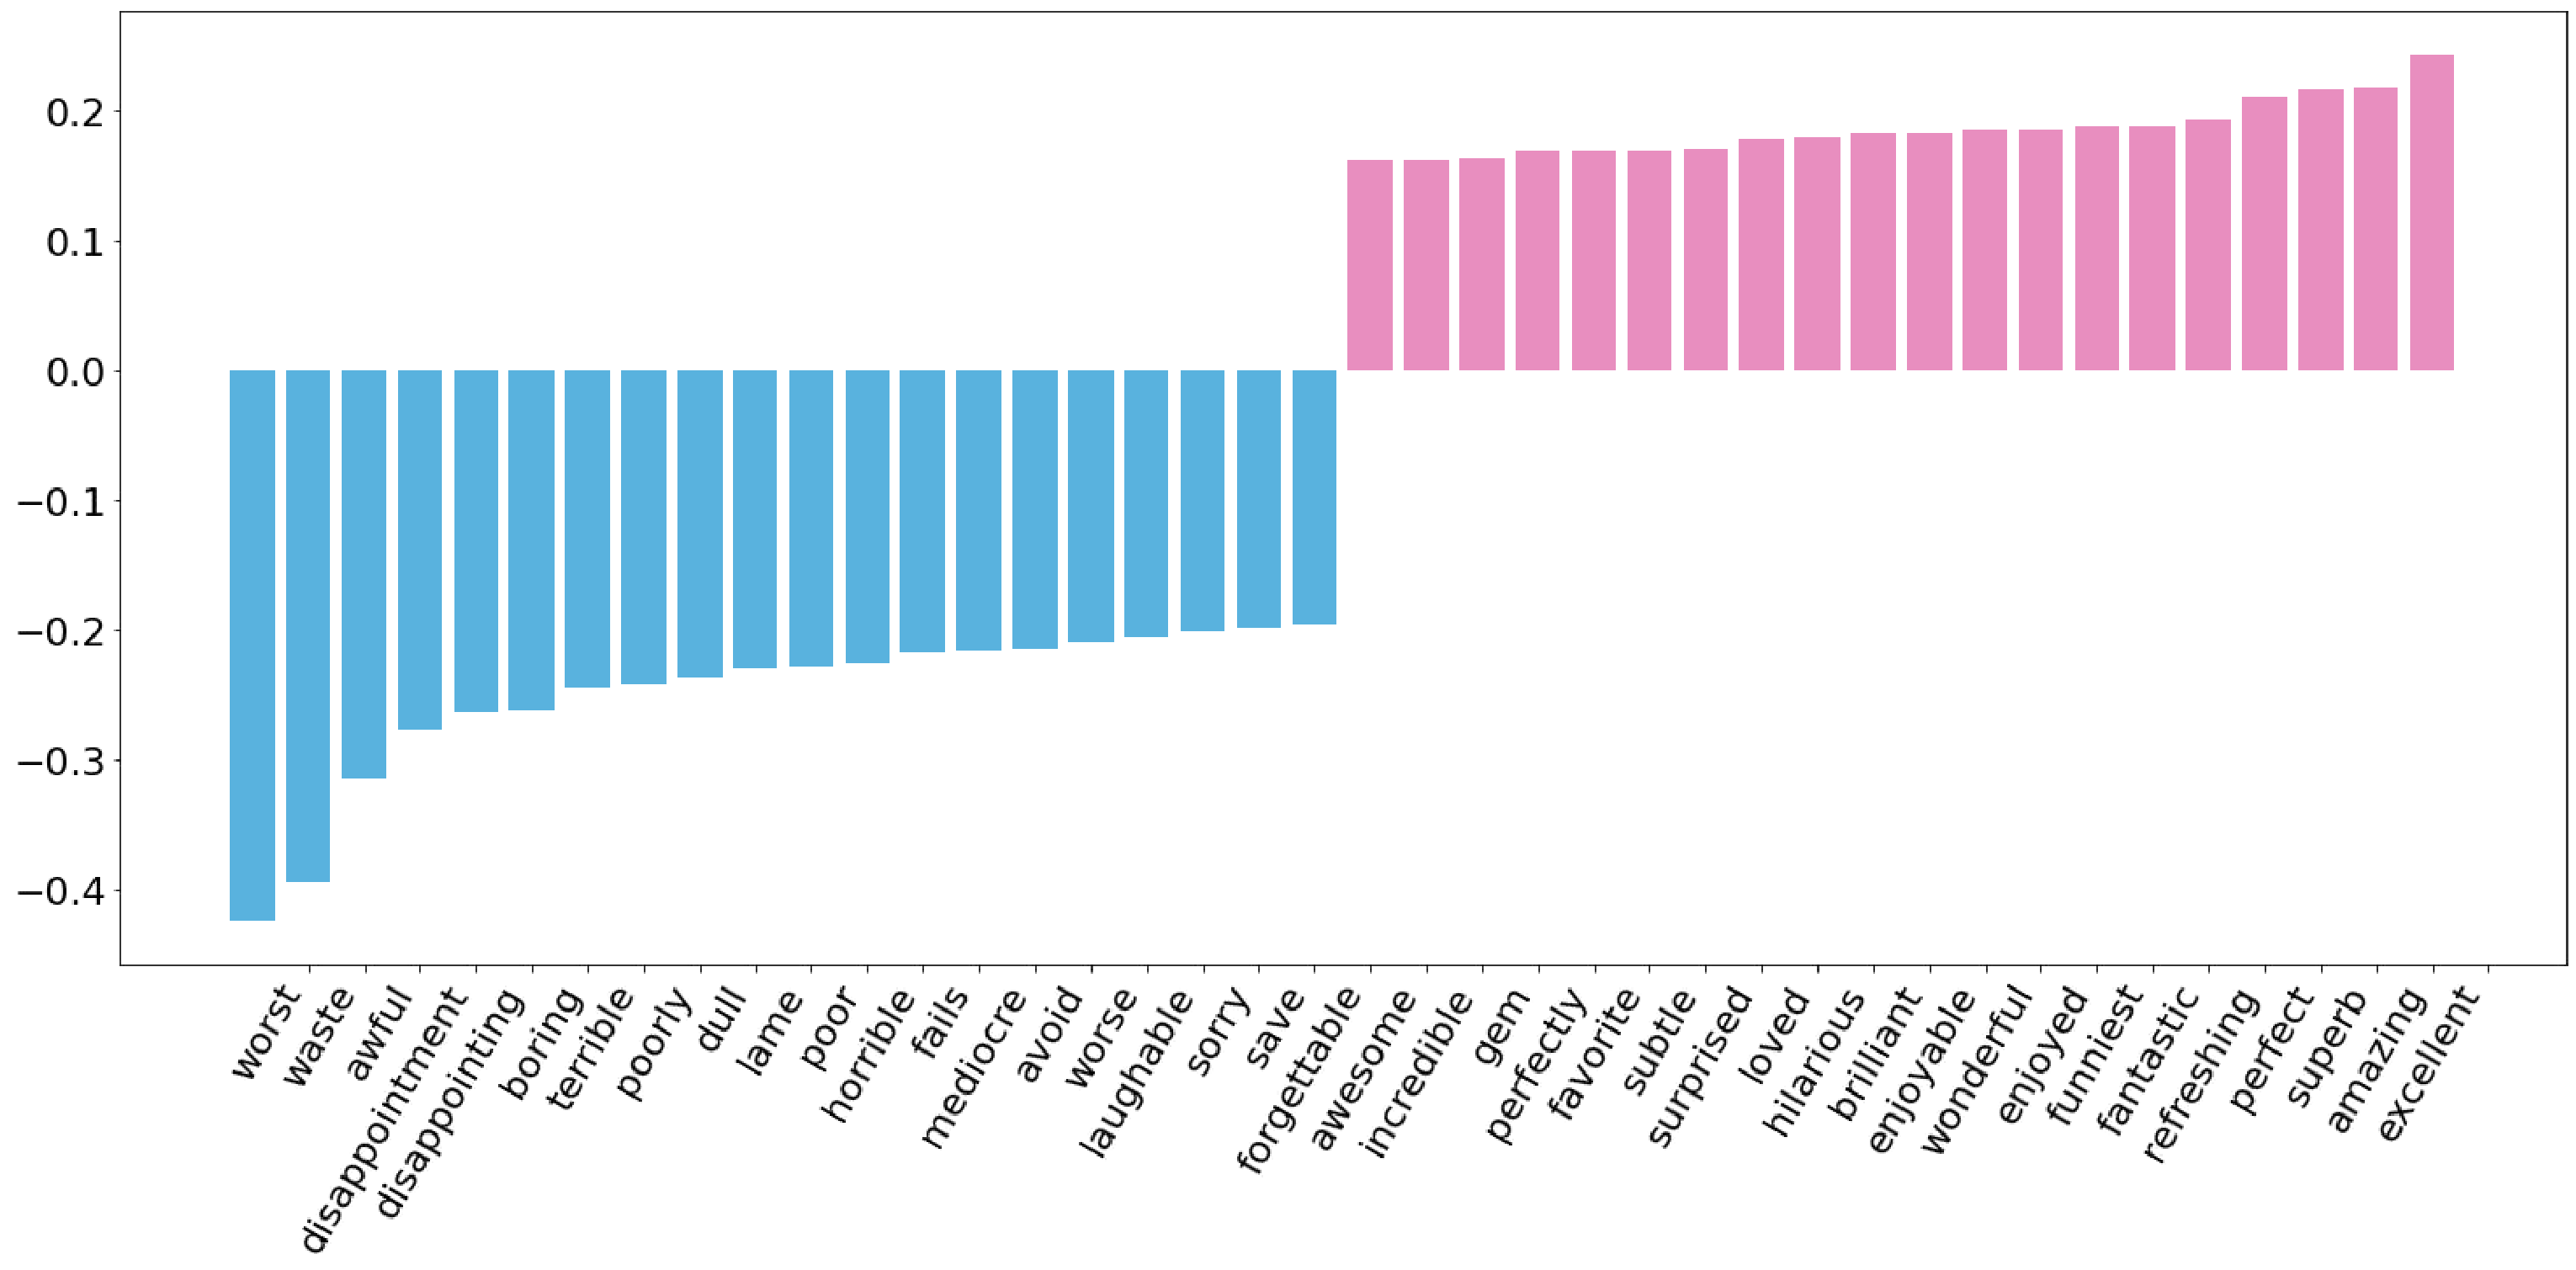
\includegraphics[width=1\linewidth]{images/chapter3/svc-visual.pdf}
	\caption{Wizualizacja wydźwięku pozytywnego lub negatywnego wyrazów (SVM).}
	\label{fig:visual-svc}
\end{figure}



\subsection{Sieci neuronowe}
W kolejnych etapach stworzyłysmy modele sieci neuronowych a dokładniej konwolucyjnej sieci neuronowej (subsekcja \ref{subsec:cnn}), sieci LSTM --- długoterminowej pamięci krótkoterminowej, która jest typem sieci rekurencyjnej (sekcja \ref{sec:lstm}) oraz zamodelowałyśmy wyniki połączenia tych dwóch rodzajów sieci razem (sekcja \ref{sec:cnn-lstm}).

\noindent Jako że użycie sieci neuronowych wymaga najpierw wyrażenia każdego słowa w postaci wektora liczb (\textit{embedding}), zastosowałyśmy metodę Word2Vec \cite{mikolov2013efficient}. Żeby osiągnąć pożądany rezultat zaimplementowałysmy metodą \verb|get_lists_of_words(data)|, do której zaaplikowałyśmy nasze dane treningowe i w rezultacie otrzymałyśmy listę słów.

\begin{lstlisting}[language=Python,frame=single, breaklines=true, caption=Stworzenie listy słów dla modelu Word2Vec.,label=code:w2v-wordlist]
import re
def get_lists_of_words(data):
	clean_reviews = data.map(lambda review: re.sub(r'([^a-z|\s])+', '', review.lower()))
	return [review.split() for review in clean_reviews]

train_data_list_of_words = get_lists_of_words(train_data)
\end{lstlisting}	

\noindent Następnie wytrenowałysmy model \verb|Word2Vec| na tej stworzonej liście słów.
\begin{lstlisting}[language=Python,frame=single, breaklines=true, caption=Trenowanie modelu Word2Vec.,label=code:w2v]
import gensim
word2vec_model = gensim.models.Word2Vec(
				train_data_list_of_words,
				size=150,  
				window=10, 
				min_count=2, 
				workers=10
				)

word2vec_model.train(train_data_list_of_words,total_examples=len(train_data_list_of_words),epochs=10)
\end{lstlisting}

\noindent Wytrenowane wektory słów są przechowywane w instancji KeyedVectors jako, w naszym przypadku, \verb|word2vec_model.wv|. Ten obiekt zasadniczo zawiera mapowanie między słowami i osadzaniami/ zagłębieniami (\textit{embeddings}).


\noindent Pakiet gensim zapewnia też wiele przydatnych metod. Na przykład dzięki metodzie \verb|most_similar('słowo')| umożliwia znajdowanie słów najbardziej zbliżonych do podanego w parametrze słowa (Listing. \ref{code:similar-different}, linia 1) oraz dzięki metodzie \verb|doesnt_match| \verb|([słowa])| słowo/a, które nie pasuje/ą do reszty słów na liście (Listing. \ref{code:similar-different}, linia 2).

\begin{lstlisting}[language=Python,frame=single, breaklines=true, caption=Znajdowanie najbardziej zbliżonych i nie pasujących słów.,label=code:similar-different]
word2vec_model.wv.most_similar('actor')
word2vec_model.wv.doesnt_match(['good', 'nice','small', 'fine'])
\end{lstlisting}

\noindent Słowa najbardziej zbliżone do słowa actor:
\begin{Verbatim}
[('actress', 0.5977960824966431),
('performer', 0.5925692915916443),
('role', 0.5761367678642273),
('comedian', 0.5694815516471863),
('performance', 0.5201245546340942),
('newcomer', 0.4978533387184143),
('actors', 0.4970739483833313),
('impersonation', 0.47669658064842224),
('thespian', 0.47024333477020264),
('foxx', 0.46994471549987793)]
\end{Verbatim}

\noindent Słowo nie pasujące do reszty:
\begin{Verbatim}
small
\end{Verbatim}

\begin{lstlisting}[language=Python,frame=single, breaklines=true, caption=Generacja wektora słów --- model Word2Vec.,label=code:w2v-results]
word_vectors = pd.DataFrame(word2vec_model[word2vec_model.wv.vocab], word2vec_model.wv.vocab)
\end{lstlisting}

%%%  ------------> obrazek
\begin{figure}[H]
	\centering
	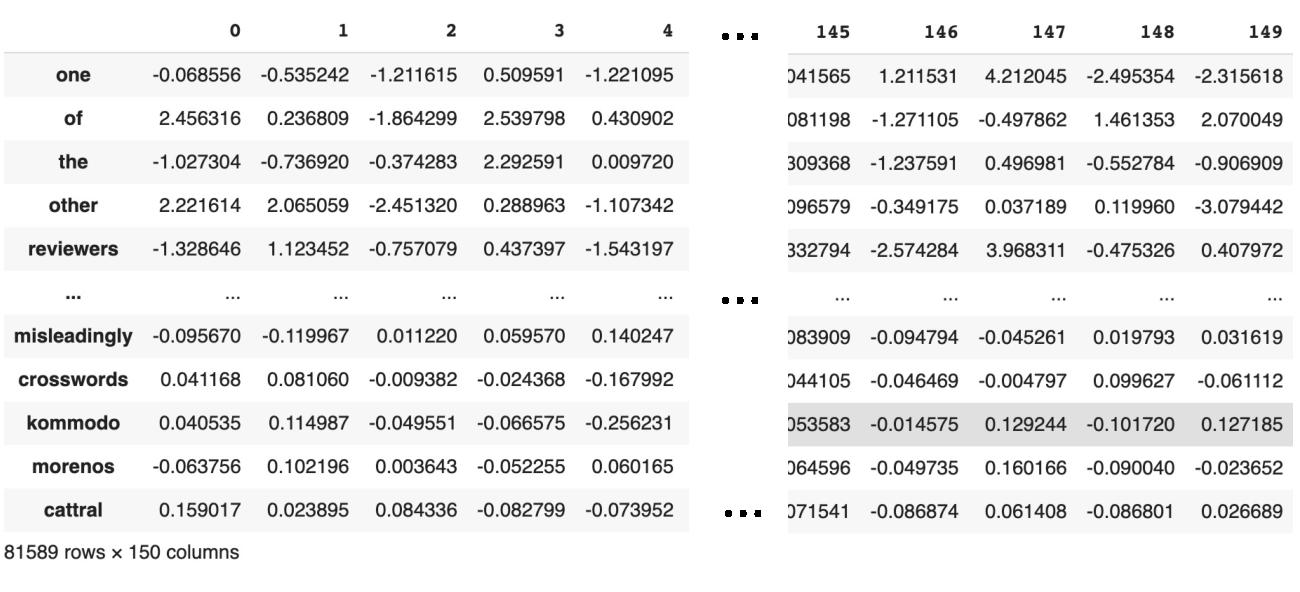
\includegraphics[width=1\linewidth]{images/chapter3/w2v-dframe.pdf}
	\caption{Wyniki modelu Word2Vec --- wektory słów, dla size=150.}
	\label{fig:w2v-dframe}
\end{figure}

\noindent Rezultaty działania modelu można również wizualizować, ale najpierw należy zmniejszyć wymiarowość wektorów --- w naszym przypadku ze 150 wymiarów do 2. Można to zrobić przy użyciu klasy \verb|TSNE| z pakietu \verb|sklearn.manifold| (Listing. \ref{code:tsne}), która pozwoli wygenerować odpowiednie punkty, które można później przedstawić w formie wykresu.

\begin{lstlisting}[language=Python,frame=single, breaklines=true, caption=Zmniejszenie wymiarowości wektorów słów do punktów.,label=code:tsne]
from sklearn.manifold import TSNE
tsne = TSNE(perplexity = 30, n_components=2, init='pca', n_iter=50000, method='exact')tsne = TSNE(perplexity = 30, n_components=2, init='pca', n_iter=50000, method='exact')

points = tsne.fit_transform(np.array(word_vectors)[1000:1500,:])
\end{lstlisting}

\noindent Możliwe jest wygenerowanie wykresu/ grafiki, na której zaznaczone są słowa (wszystkie lub wybrany podzbiór). Słowa o podobnym znaczeniu powinny tworzyć skupiska --- znajdować się blisko siebie. Jednakże, jeżeli stworzy się taką grafikę dla zbyt dużej liczby słów, to staje się ona mało czytelna. Idea tej wizualizacji dla 500 przykładowych słów z naszego zbioru znajduje się poniżej (Rysunek. \ref{fig:w2v-kropki}). Jak widać, przy tym powiększeniu grafika ta jest mało użyteczna. Po odpowiednim (dużym) powiększeniu można znaleźć pewne skupiska słów i zależności.

%%%  ------------> obrazek
\begin{figure}[H]
	\centering
	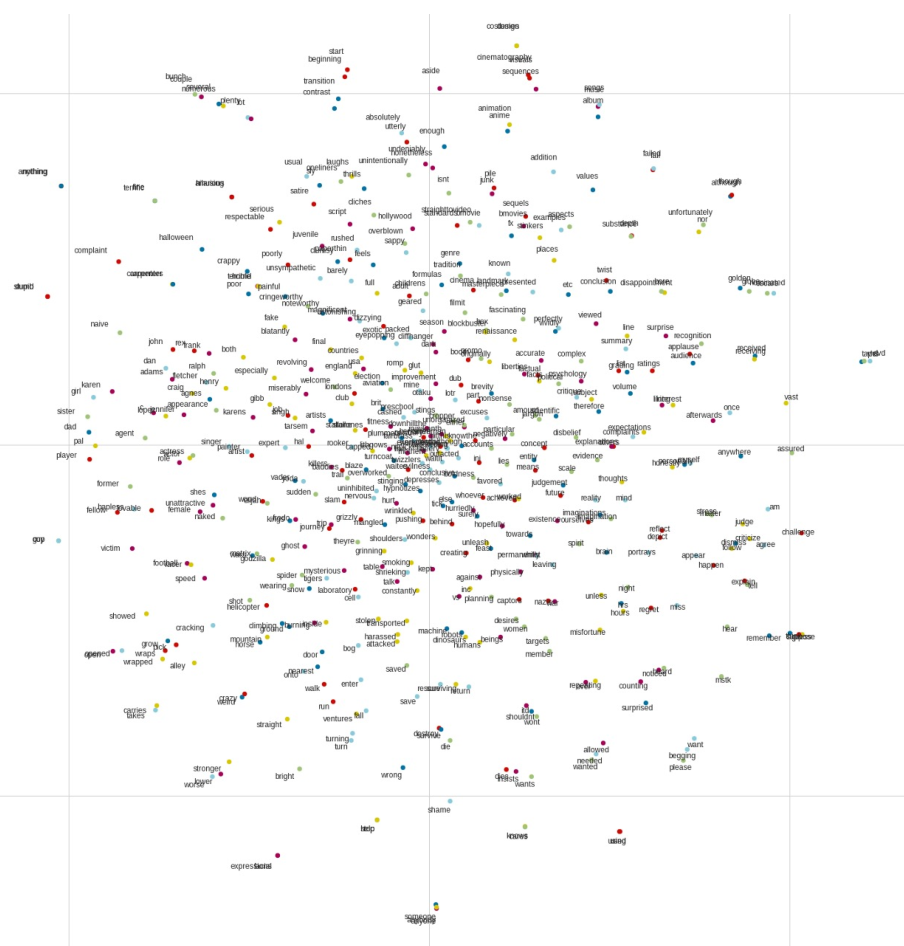
\includegraphics[width=0.95\linewidth]{images/chapter3/w2v-kropki.pdf}
	\caption{Wizualizacja W2V}
	\label{fig:w2v-kropki}
\end{figure}


\noindent Podobnie może być przydatny również rozkład długości recenzji (wyrażony jako liczba słów w recenzji).  Taką zależnośc również można zwizualizować z zaznaczeniem wybranych percentyli (Rysunek. \ref{fig:w2v-percentyle}). W naszym przypadku łatwo zauważyć, że połowa recenzji ma 170 słów lub mniej, 25\% recenzji ma długość między 171 a 273 słowa, kolejne 15\% recenzji ma długość pomiędzy 274 a 441 słów, a 10\% jest dłuższych niż 441 słów. Wyraźnie dominują tu recenzje krótkie. W sumie 75\% recenzji jest co najwyżej średniej długości (do 273 słów).

%%%  ------------> obrazek
\begin{figure}[H]
	\centering
	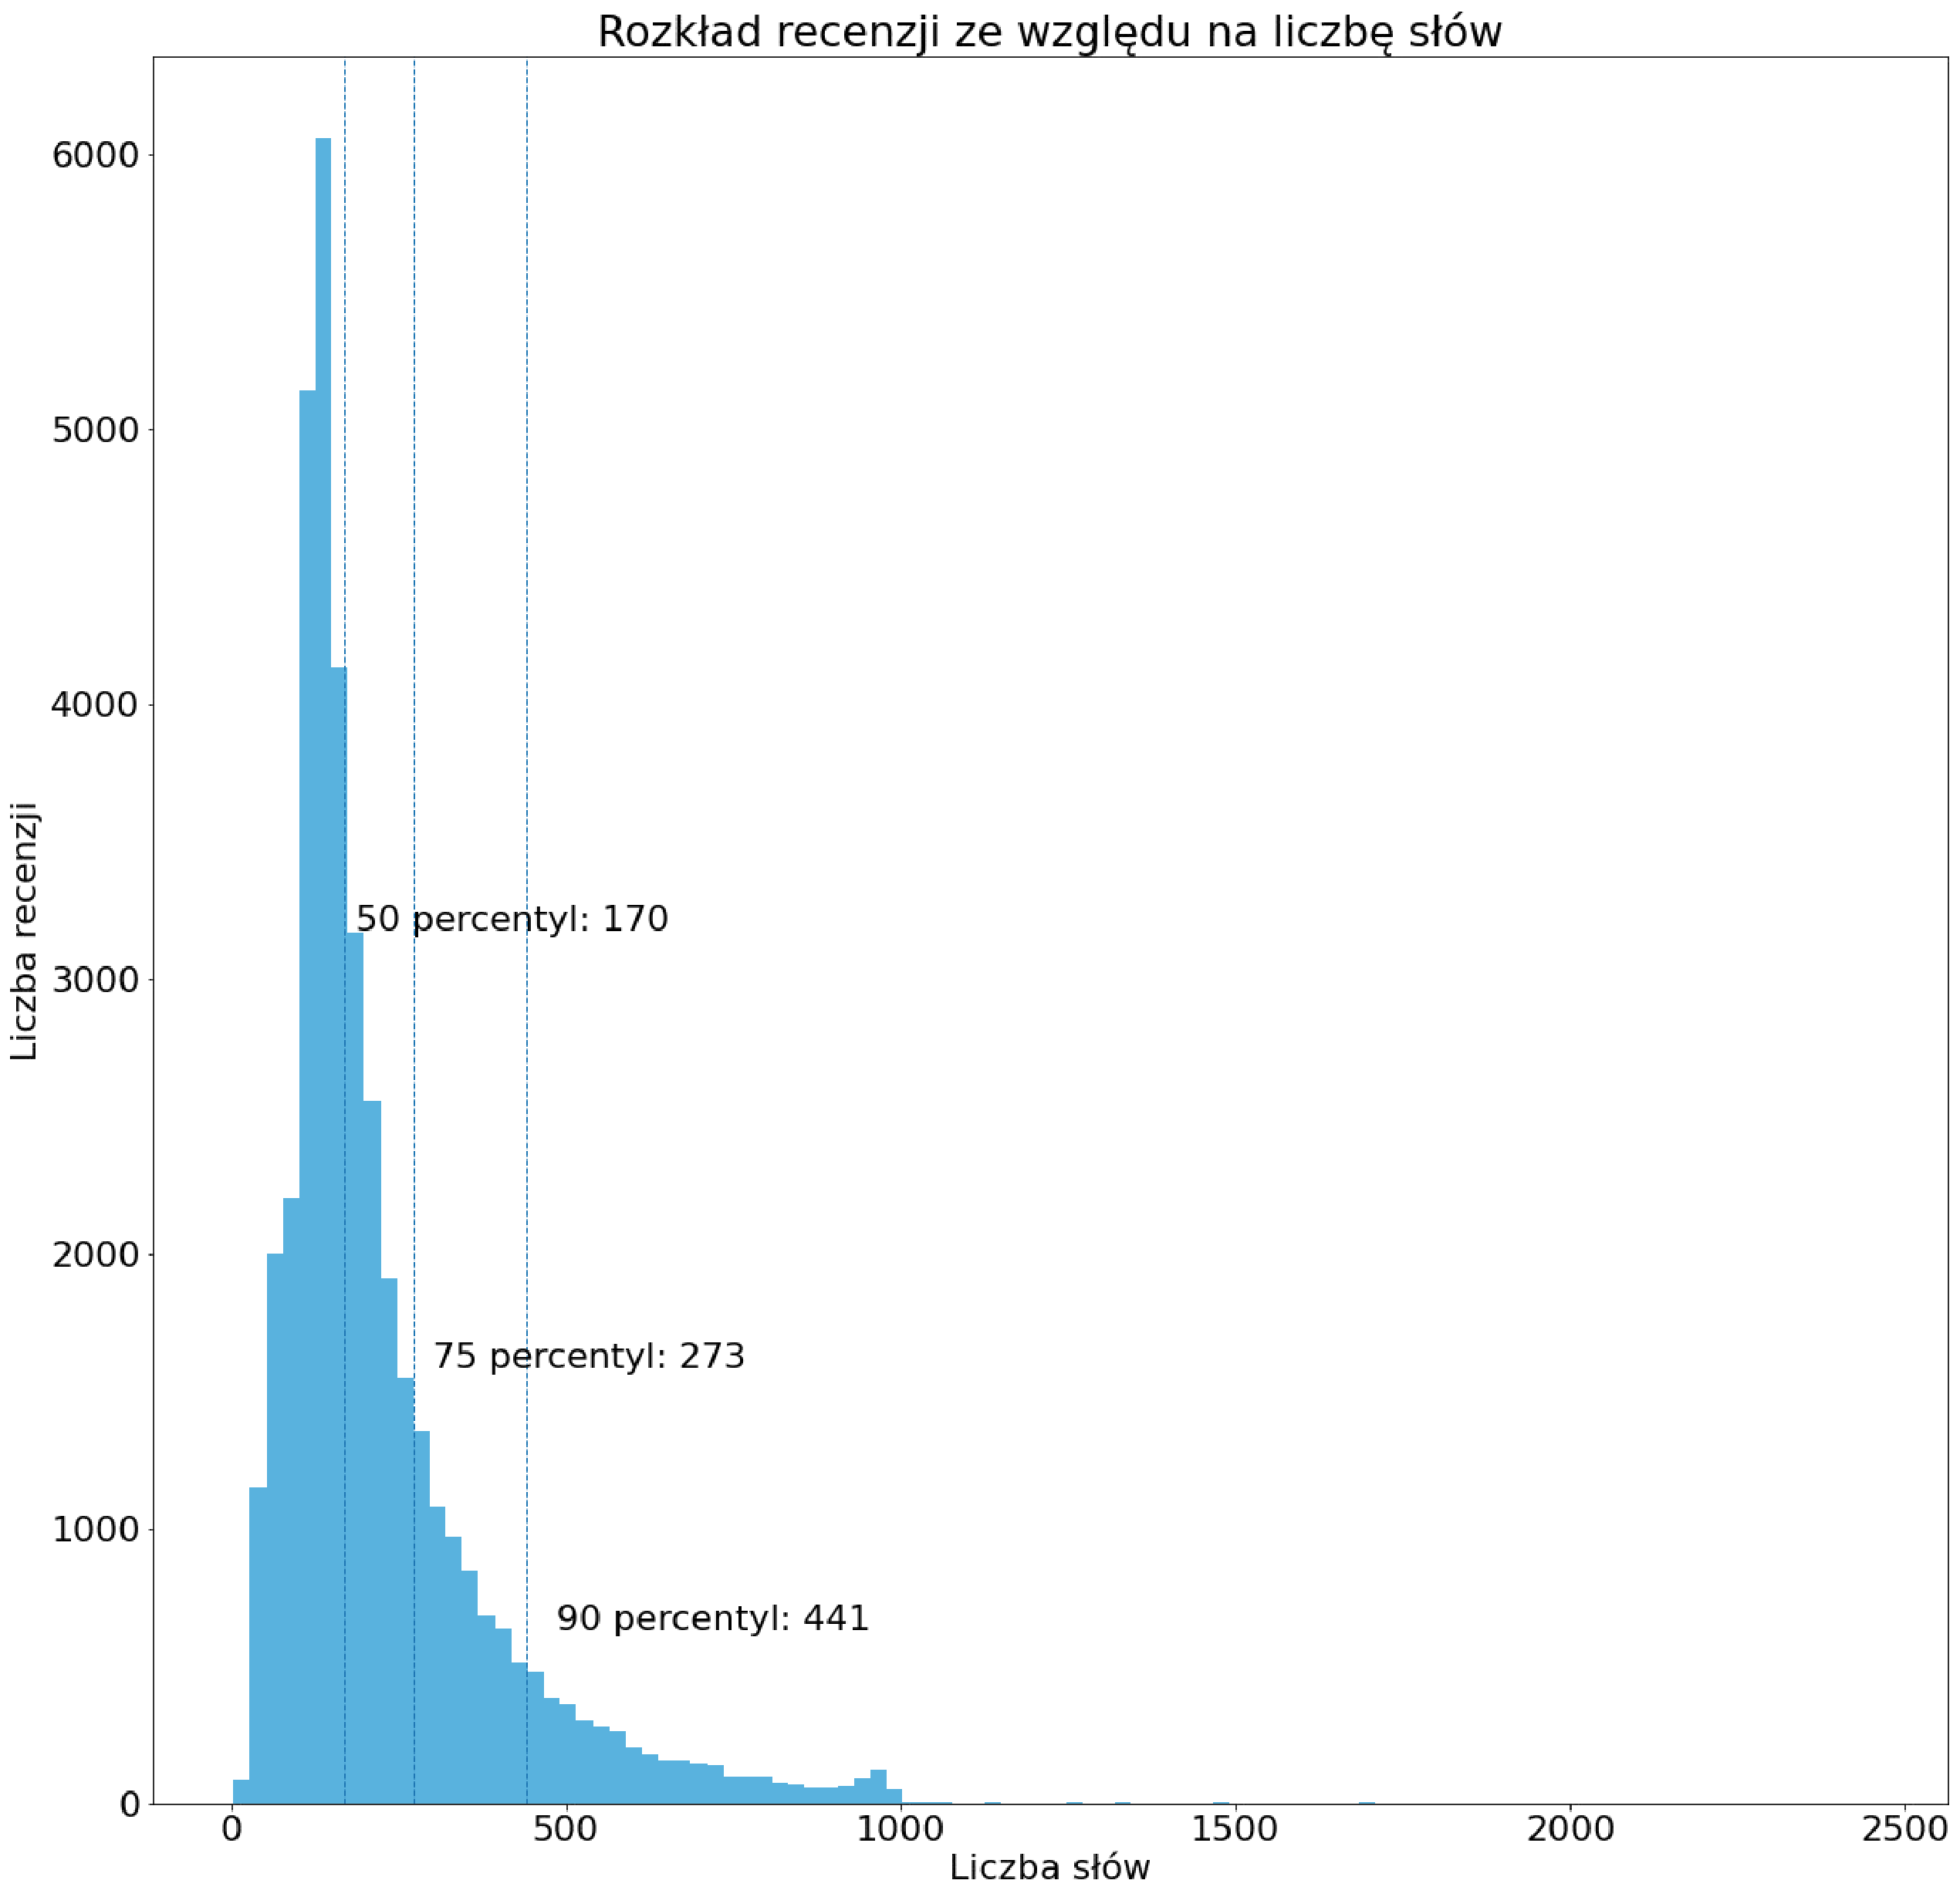
\includegraphics[width=0.75\linewidth]{images/chapter3/w2v-percentyle.pdf}
	\caption{Wizualizacja rozkładu liczby słów w recenzjach.}
	\label{fig:w2v-percentyle}
\end{figure}

\noindent Tak więc tworząc macierze danych do trenowania modeli sieci neuronowych ustaliłyśmy 273 słowa jako górną granicę (maksymalny wymiar).

\subsubsection{Konwolucyjna sieć neuronowa}

\noindent W wyniku wykonania szeregu przekształceń (dokładna procedura znajduje się w notebooku Google Colab w części Data Preparation dla sieci neuronowych) otrzymałyśmy dwie macierze danych treningową --- \verb|train_data_matrix| i testową --- \verb|test_data_matrix|.
Następnie zdefiniowałysmy funkcję \verb|cnn_model| i przy użyciu biblioteki \verb|keras| stworzyłyśmy model konwolucyjnej sieci neuronowej. W warstwie konwolucyjnej wykorzystałyśmy 128 filtrów o długości 5 oraz funkcję aktywacji ReLu. Następnie, wykorzystałyśmy warstwę \textit{global max pooling} oraz \textit{dropout} z prawdopodobieństwen 0.2.  Użyłyśmy również 10 warstw ukrytych z funkcją aktywacji ReLu oraz ostatniej warstwy wyjściowej z sigmoidalną warstwą aktywacji (dokładne parametry na Listingu. \ref{code:cnn}). Jako funkcji straty użyłyśmy \verb|binary_crossentropy|,a metryką sukcesu ponownie zostało \verb|accuracy|.

\begin{lstlisting}[language=Python,frame=single, breaklines=true, caption=Model CNN.,label=code:cnn]
def cnn_model():
	embed_size=150
	model = Sequential()
	model.add(layers.Embedding(embedding_matrix_size + 1, embed_size, weights=[embedding_matrix]))
	model.add(layers.Conv1D(128, 5, activation='relu'))
	model.add(layers.GlobalMaxPooling1D())
	model.add(layers.Dropout(0.2))
	model.add(layers.Dense(10, activation='relu'))
	model.add(layers.Dense(1, activation='sigmoid'))
	
	model.compile(loss='binary_crossentropy',
	metrics=['accuracy'])
	
	return model
\end{lstlisting}

\begin{Verbatim}
Model: 'Sequential'
Layer (type)                 Output Shape              Param #   
=================================================================
embedding_6 (Embedding)      (None, None, 150)         10894350  
_________________________________________________________________
conv1d_6 (Conv1D)            (None, None, 128)         96128     
_________________________________________________________________
global_max_pooling1d_6 (Glob (None, 128)               0         
_________________________________________________________________
dropout_4 (Dropout)          (None, 128)               0         
_________________________________________________________________
dense_12 (Dense)             (None, 10)                1290      
_________________________________________________________________
dense_13 (Dense)             (None, 1)                 11        
=================================================================
Total params: 10,991,779
Trainable params: 10,991,779
Non-trainable params: 0
\end{Verbatim}

\noindent Powyższy model został skompilowany. Jak widać składa się z prawie 11 milionów trenowalnych parametrów, a następnie wytrenowany. 

\begin{lstlisting}[language=Python,frame=single, breaklines=true, caption=Trening modelu CNN.,label=code:cnn-trening]
cnn_model = cnn_model().fit(
			train_data_matrix,
			train_labels,
			epochs=8,
			verbose=True,
			batch_size=100
			)
\end{lstlisting}

\begin{Verbatim}
Epoch 1/8 - 169s 418ms/step - loss: 0.5815 - accuracy: 0.6748
Epoch 2/8 - 166s 416ms/step - loss: 0.3491 - accuracy: 0.8466
Epoch 3/8 - 166s 415ms/step - loss: 0.2954 - accuracy: 0.8750
Epoch 4/8 - 166s 414ms/step - loss: 0.2593 - accuracy: 0.8930
Epoch 5/8 - 166s 415ms/step - loss: 0.2279 - accuracy: 0.9069
Epoch 6/8 - 165s 412ms/step - loss: 0.1989 - accuracy: 0.9192
Epoch 7/8 - 164s 409ms/step - loss: 0.1729 - accuracy: 0.9316
Epoch 8/8 - 165s 412ms/step - loss: 0.1499 - accuracy: 0.9415
\end{Verbatim}

\noindent Ostatnią czynnością jaką zrobiłyśmy dla tego modelu była predykcja klas w oparciu o zbiór testowy (Listing. \ref{code:cnn-pred}).

\begin{lstlisting}[language=Python,frame=single, breaklines=true, caption=Predykcja z użyciem modelu CNN.,label=code:cnn-pred]
cnn_predictions = cnn_model.predict_classes(test_data_matrix)
\end{lstlisting}

\noindent Wyniki przedstawione są w macierzy omyłek (Rysunek. \ref{fig:cnn-macierz}).

\noindent Kolorem granatowym zostały oznaczone wartości przewidziane prawidłowo przez skonstruowany przez nas model --- 4412 wartości zostały zaklasyfikowane prawidłowo jako pozytywne i 4512 wartości zostały zaklasyfikowane prawidłowo jako negatywne, co po zsumowaniu daje 8924 prawidłowo sklasyfikowane wartości na 10~000 przykładów. Tak więc precyzja predykcji wynosi 89.24\%. Ponadto 532 przykładów zostało błędnie sklasyfikowanych jako pozytywne i 544 błędnie jako negatywne (ćwiartki w kolorze błękitnym). Całkowity czas trenowania modelu zajął tutaj nieco ponad 22 minuty (średnio około 2 minuty i 46 sekund na 1 epokę). Jest to czas dłuższy niż dla dotychczasowych dwóch modeli, ale trzeba tu podkreślić, że model ten posiadał prawie 11 milionów trenowalnych parametrów.
%%%  ------------> obrazek
\begin{figure}[H]
	\centering
	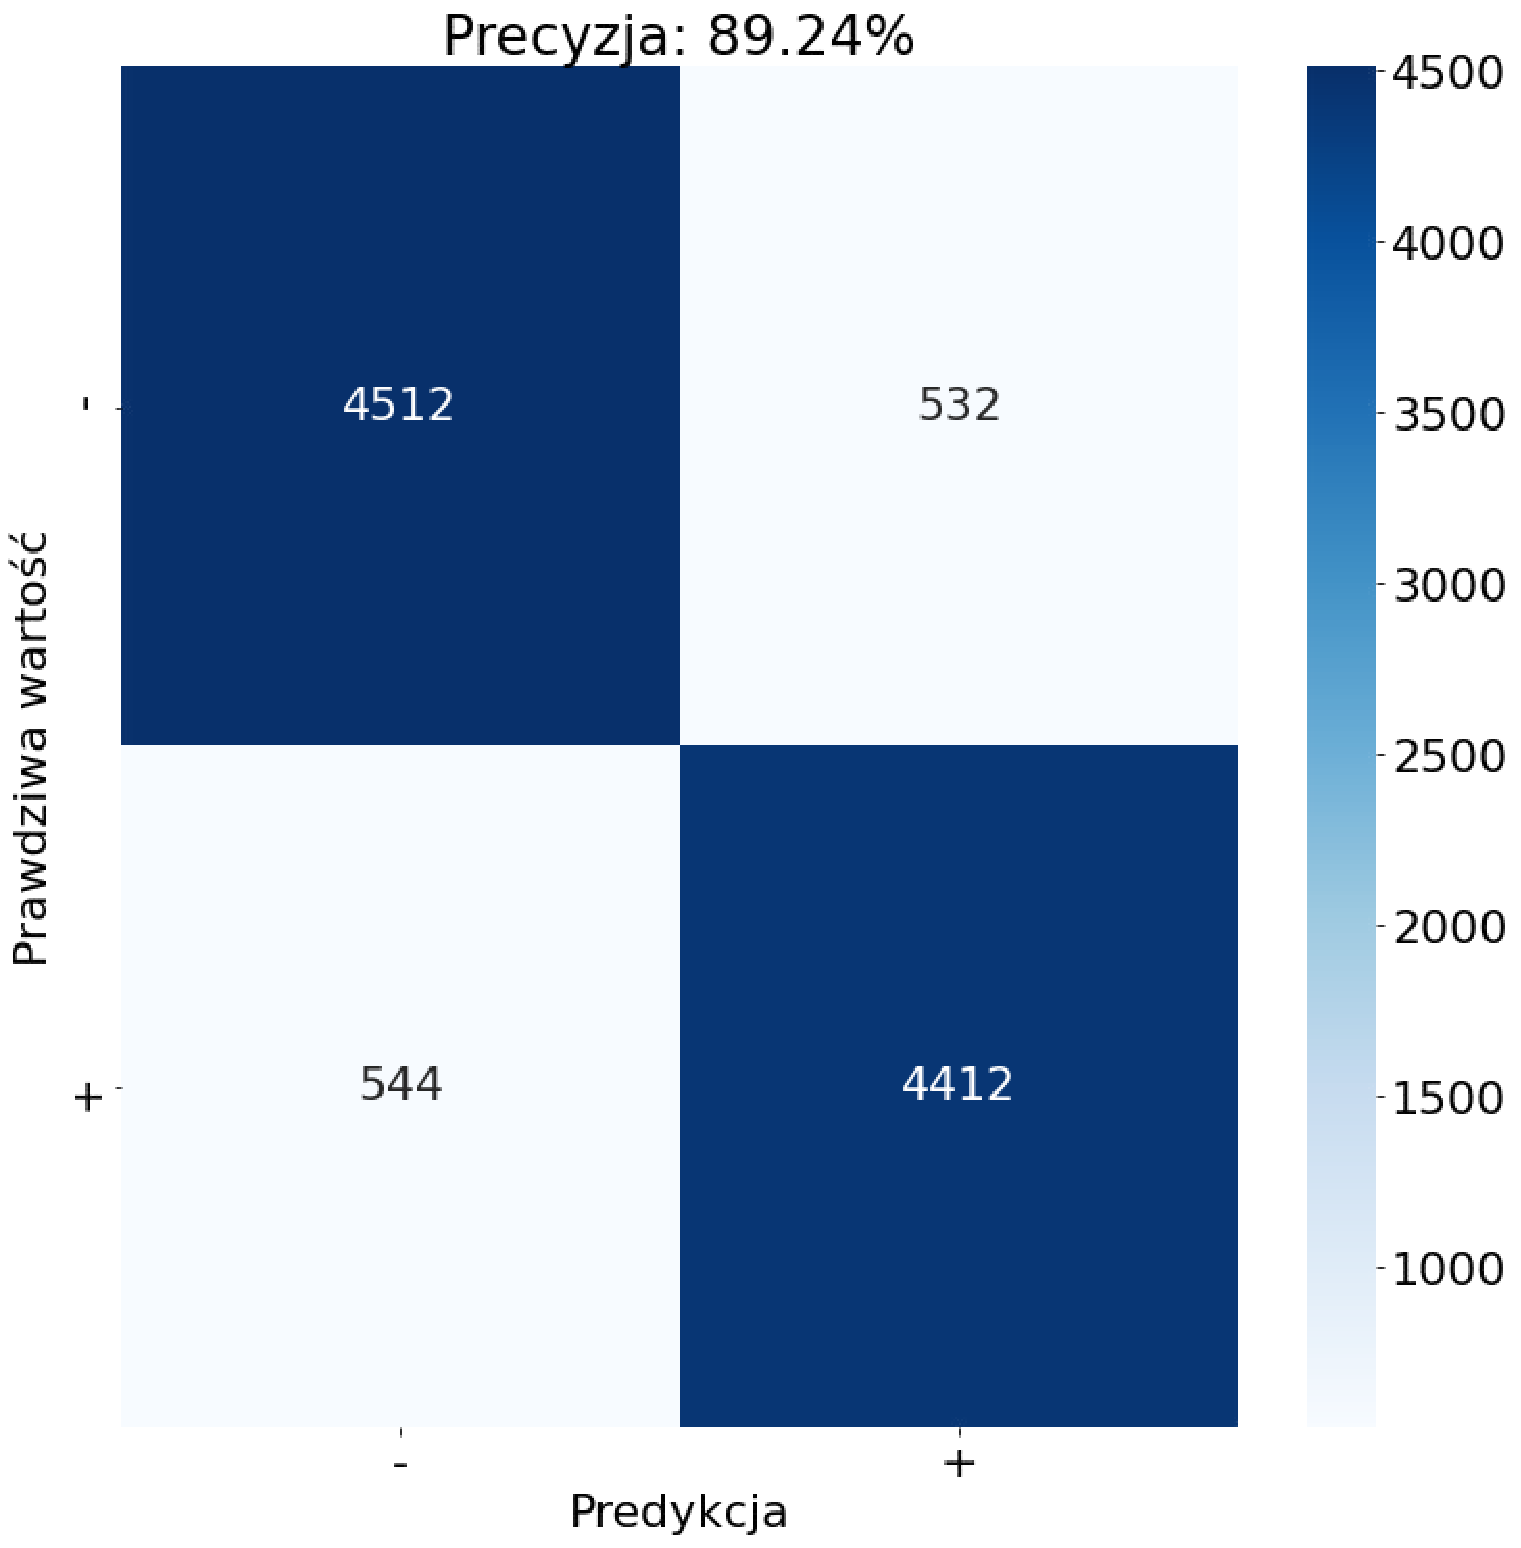
\includegraphics[width=0.5\linewidth]{images/chapter3/cnn-macierz.pdf}
	\caption{Wyniki klasyfikacji z użyciem konwolucyjnej sieci neuronowej.}
	\label{fig:cnn-macierz}
\end{figure}




%----------------- LSTM ----------------
\subsubsection{LSTM}

Model LSTM został zaimplementowany podobnie jak model konwolucyjny z użyciem \verb|Sequential()|. Zdefiniowałyśmy funkcję \verb|model_lstsm| i przy użyciu biblioteki \verb|keras| stworzyłyśmy model sieci neuronowej LSTM. Zamiast warstwy konwolucyjnej, używamy tutaj warstwy LSTM z wektorem wyjściowym o długości 128. Jako że jest to model rekurencyjny ustawiłyśmy dodatkowy parametr \verb|recurrent_dropout| na wartość 0.2. Ostatnia warstwa --- wyjściowa ma sigmoidalną aktywację (dokładne parametry na Listingu. \ref{code:lstm}). Jako funkcji straty ponownie użyłyśmy \verb|binary_crossentropy|, a jako metryki sukcesu \verb|accuracy|.

\begin{lstlisting}[language=Python,frame=single, breaklines=true, caption=Model LSTM.,label=code:lstm]
def lstsm_model():
	embed_size=150
	model = Sequential()
	model.add(layers.Embedding(embedding_matrix_size + 1, embed_size, weights=[embedding_matrix]))
	model.add(layers.LSTM(128, dropout=0.2, recurrent_dropout=0.2))
	model.add(layers.Dense(1, activation='sigmoid'))
	print(model.summary())
	model.compile(loss='binary_crossentropy',
	metrics=['accuracy'])
	return model
\end{lstlisting}

\newpage
\begin{Verbatim}
Model: 'Sequential'
Layer (type)                 Output Shape              Param #   
=================================================================
embedding_4 (Embedding)      (None, None, 150)         10894350  
_________________________________________________________________
lstm (LSTM)                  (None, 128)               142848    
_________________________________________________________________
dense_8 (Dense)              (None, 1)                 129       
=================================================================
Total params: 11,037,327
Trainable params: 11,037,327
Non-trainable params: 0
\end{Verbatim}


\noindent Powyższy model został skompilowany. Jak widać składa się z ponad 11 milionów trenowalnych parametrów, a następnie wytrenowany. 

\begin{lstlisting}[language=Python,frame=single, breaklines=true, caption=Trening modelu LSTM.,label=code:lstm-trening]
lstm_model = lstsm_model().fit(
			train_data_matrix,
			train_labels,
			epochs=8,
			verbose=True,
			batch_size=100
			)
\end{lstlisting}

\begin{Verbatim}
Epoch 1/8 - 583s 1s/step - loss: 0.5784 - accuracy: 0.6985
Epoch 2/8 - 576s 1s/step - loss: 0.4081 - accuracy: 0.8310
Epoch 3/8 - 583s 1s/step - loss: 0.3197 - accuracy: 0.8699
Epoch 4/8 - 577s 1s/step - loss: 0.2765 - accuracy: 0.8904
Epoch 5/8 - 575s 1s/step - loss: 0.2416 - accuracy: 0.9055
Epoch 6/8 - 577s 1s/step - loss: 0.2169 - accuracy: 0.9155
Epoch 7/8 - 569s 1s/step - loss: 0.1934 - accuracy: 0.9259
Epoch 8/8 - 564s 1s/step - loss: 0.1702 - accuracy: 0.9358
\end{Verbatim}

\noindent Ostatnią czynnością jaką zrobiłyśmy dla tego modelu była predykcja klas w oparciu o zbiór testowy (Listing. \ref{code:cnn-pred}).

\begin{lstlisting}[language=Python,frame=single, breaklines=true, caption=Predykcja z użyciem modelu LSTM.,label=code:lstm-pred]
lstm_predict_data = lstm_model.predict(test_data_matrix)
\end{lstlisting}

Poniżej przedstawiłyśmy macierz omyłek.

\begin{figure}[H]
	\centering
	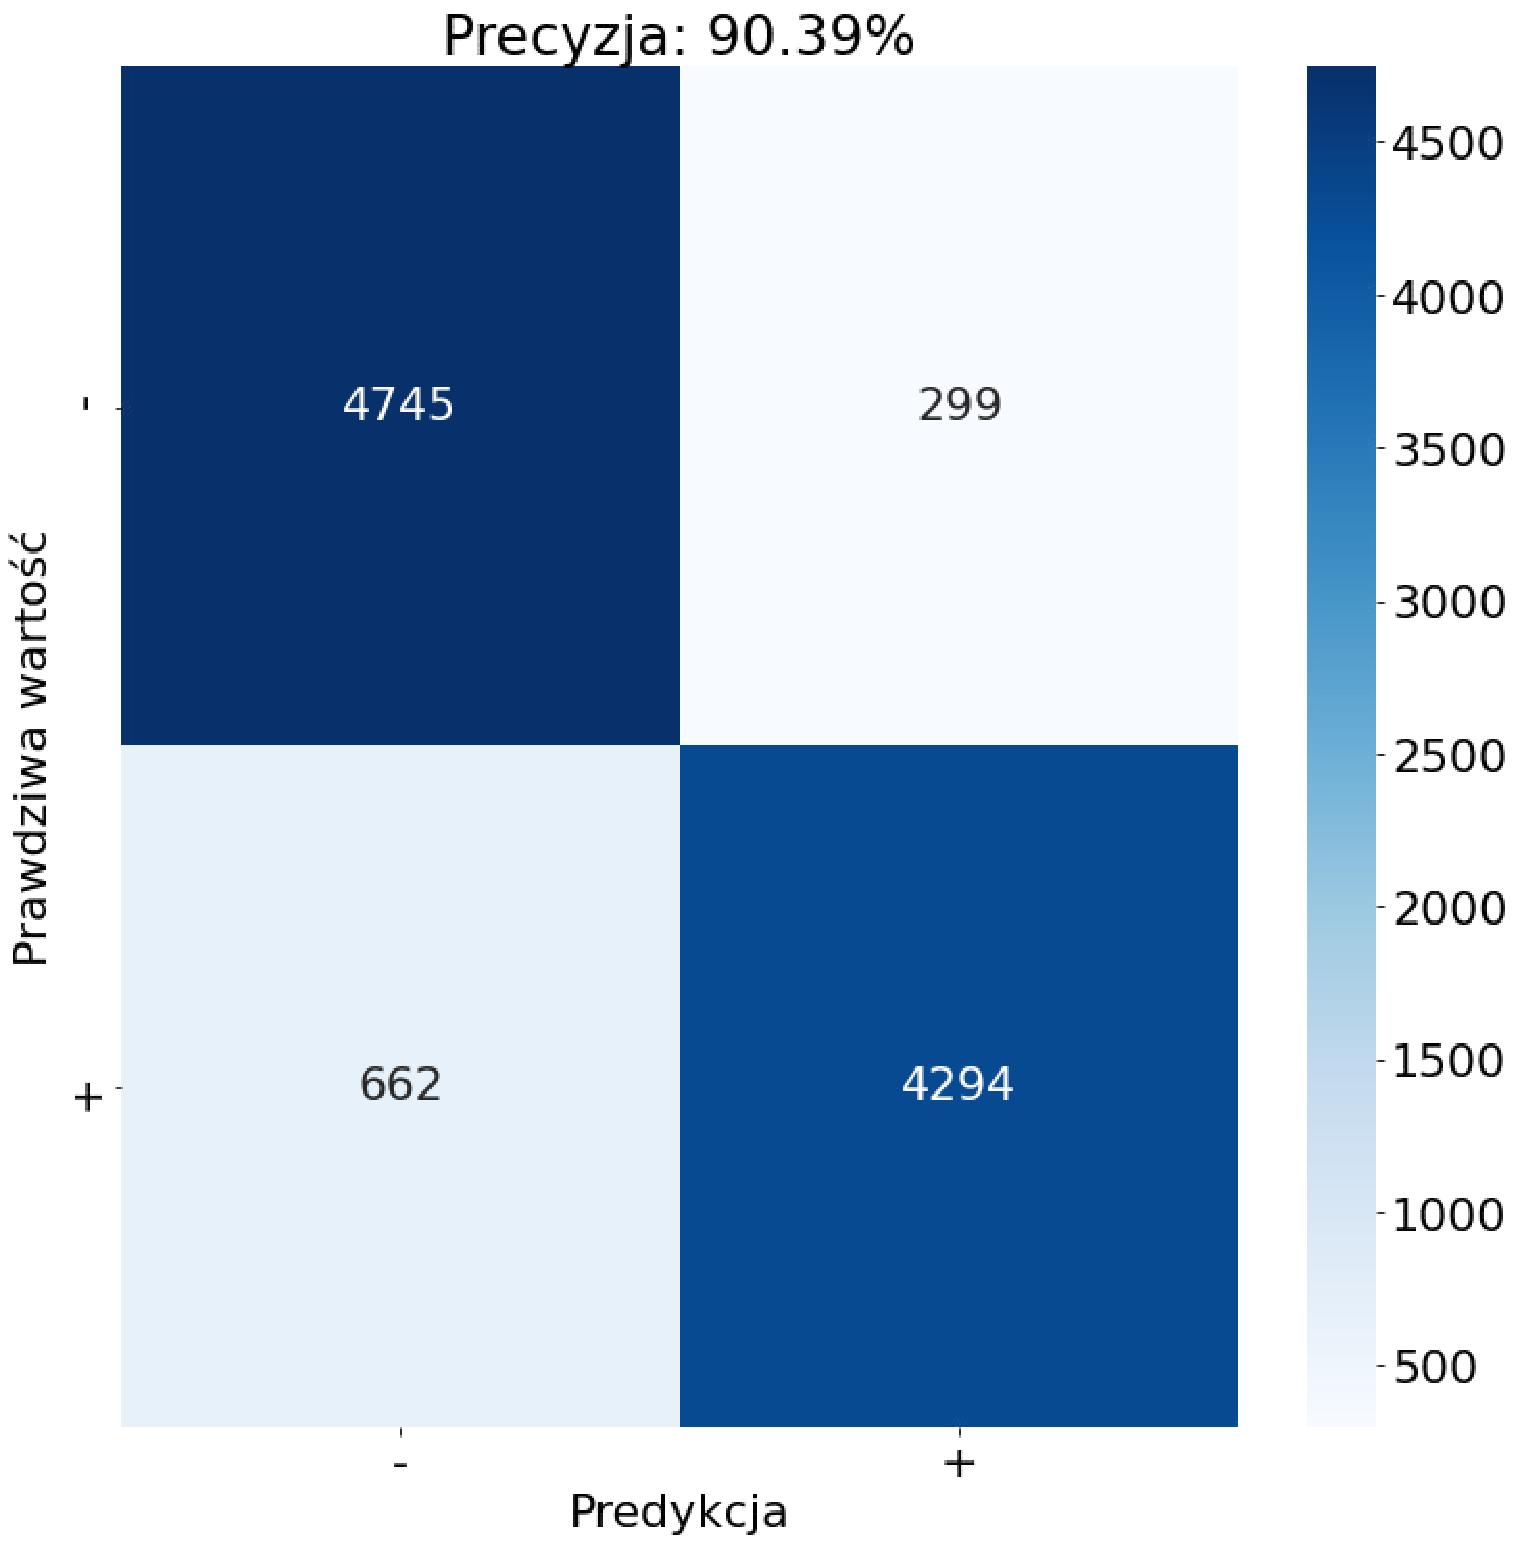
\includegraphics[width=0.5\linewidth]{images/chapter3/lstm-macierz.pdf}
	\caption{Wyniki klasyfikacji z użyciem sieci LSTM.}
	\label{fig:lstm-macierz}
\end{figure}

\noindent Kolorem granatowym zostały oznaczone wartości przewidziane prawidłowo przez skonstruowany przez nas model --- 4294 wartości zostały zaklasyfikowane prawidłowo jako pozytywne i 4745 wartości zostały zaklasyfikowane prawidłowo jako negatywne, co po zsumowaniu daje 9039 prawidłowo sklasyfikowane wartości na 10~000 przykładów. Tak więc precyzja predykcji wynosi 90.39\%. Ponadto 299 przykładów zostało błędnie sklasyfikowanych jako pozytywne i 662 błędnie jako negatywne (ćwiartki w kolorze błękitnym). Całkowity czas trenowania modelu zajął tutaj ponad 76 minut (średnio około 9 minut i 35 sekund na 1 epokę). Jest to czas znacznie dłuższy niż dla dotychczasowych modeli --- lecz model jest również najbardziej zaawansowany i składa się z ponad 11 mln parametrów.


%--------------- CNN-LSTM Ensemble -------------
\subsubsection{CNN--LSTM Ensemble}
Jako ostatnią próbę polepszenia naszych predykcji, mimo, że wartości bliskie 90\%, to bardzo wysokie wyniki, zastosowałyśmy połączenie działania modeli CNN i LSTSM (CNN-LSTM Ensemble).

\begin{lstlisting}[language=Python,frame=single, breaklines=true, caption=Model stworzony przez połączenie CCN z LSTM.,label=code:cnn-lstm]
cnn_lstm_predictions = pd.DataFrame(cnn_predict_data, columns=['CNN'], index= range(0,len(test_data)))
cnn_lstm_predictions['LSTM'] = pd.DataFrame(lstm_predict_data, index= range(0,len(test_data)))
cnn_lstm_predictions['AVG'] = cnn_lstm_predictions.mean(axis=1)
cnn_lstm_predictions['Prediction'] = np.where(cnn_lstm_predictions['AVG']>0.5, 1, 0)
cnn_lstm_predictions
\end{lstlisting}


\begin{figure}[H]
	\centering
	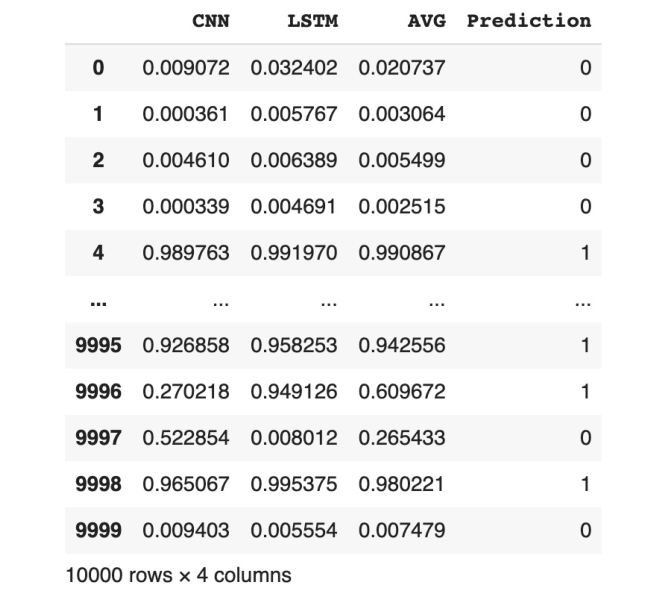
\includegraphics[width=0.55\linewidth]{images/chapter3/cnn-lstm.pdf}
	\caption{Wyniki połączenia modeli CNN i LSTM.}
	\label{fig:cnn-lstm}
\end{figure}


\noindent Zgodnie z naszą intuicją, osiągnęłyśmy pożądany efekt. Precyzja osiągnięta z tego połączenie wyniosła 90.98\%. Jest to najwyższy wynik wśród tych, które osiągnęłyśmy.

\begin{figure}[H]
	\centering
	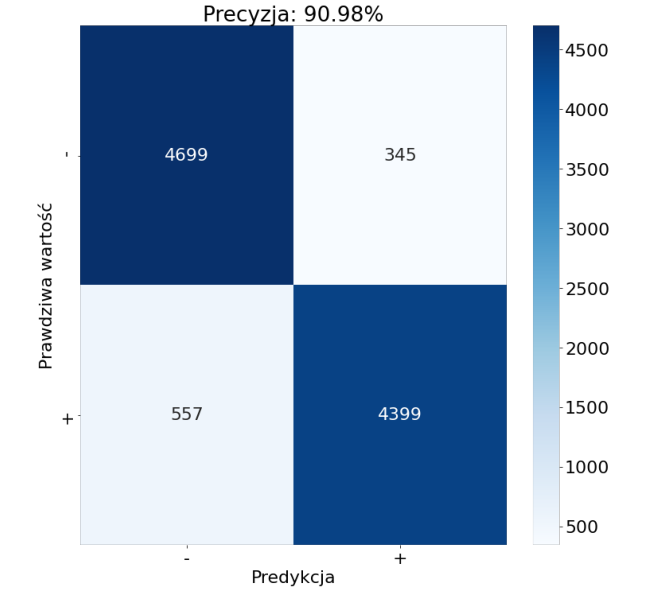
\includegraphics[width=0.55\linewidth]{images/chapter3/cnn-lstm-macierz.pdf}
	\caption{Macierz omyłek dla wyników z połączonych modeli CNN i LSTM.}
	\label{fig:cnn-lstm-macierz}
\end{figure}

\noindent Tradycyjnie kolorem granatowym zostały oznaczone wartości przewidziane prawidłowo przez skonstruowany przez nas model --- 4399 wartości zostały zaklasyfikowane prawidłowo jako pozytywne i 4699 wartości zostały zaklasyfikowane prawidłowo jako negatywne, co po zsumowaniu daje 9098 prawidłowo sklasyfikowane wartości na 10~000 przykładów. Tak więc precyzja predykcji wynosi 90.98\%. Ponadto 345 przykładów zostało błędnie sklasyfikowanych jako pozytywne i 557 błędnie jako negatywne. Został tu osiągnięty najlepszy wynik jeżeli chodzi o precyzję predykcji. Jednakże minus jest tu taki, że trzeba wytrenować zarówno sieć konwolucyjną jak i rekurencyjną, co sumarycznie zajmuje znacznie więcej czasu niż zajmowało to dla prostszych modeli, które dawały nie dużo gorsze wyniki. 

\section{Porównanie wyników dla wszystkich modeli}
W celu wyciągnięcia finalnych wniosków, porównałyśmy niektóre odpowiadające parametry stworzonych przez nas modeli. Te najważniejsze i decydujące zostały zestawione w poniższej tabeli (Tabela. \ref{tab:porównanie}). Modele posortowane zostały na podstawie precyzji --- od najmniej wydajnego do najbardziej wydajnego. 

\begin{table} [H]
	\caption{Porównanie czasów trenowania i precyzji wszystkich 5 modeli.}
	\label{tab:porównanie}
	\begin{center}
		\begin{tabular}{c | c c c c c c}
			\hline
			&  RF (D=32)      &  RF (D=64)  &       CNN         &     SVM         &    LSTM        &    CNN--LSTM \\
			\hline
			czas         &  4 min.       &   14 min.         &      22 min.     &     1 sek.        &    76 min.     &   22 + 76 min. \\
			precyzja  &  86.65\%       &    87.04\%     &    89.24\%     &     89.44\%    &   90.39\%     &     90.98\% \\
			\hline
		\end{tabular}  \\
		{\scriptsize 	RF --- Random Forest Classifier (maksymalna głębokość = 32 lub 64), SVM --- Support Vector Machine Classifier, CNN --- Convolutional Neural Network, LSTM --- Long Short-Term Memory\\}
	\end{center}
\end{table}

\noindent Nie zawsze bardziej skomplikowany model jest lepszy. W przypadku naszego zbioru danych oraz modeli widać, że różnice w precyzjach między skrajnymi modelami wynoszą tylko 4.33\%, natomiast czasy trenowania tych modeli znacznie się różnią. Pytaniem, które się tu nasuwa jest: jak by się wydłużyły te czasy gdybyśmy miały do czynienia z milionami przykładów trenujących? Należy się więc zawsze zastanowić, czy nie użyć prostszego modelu o nieco gorszej precyzji zyskując na czasie? \\
Godne uwagi jest działanie modelu klasyfikacyjnego wykorzystującego maszynę wektorów nośnych. Jak widać prosty liniowy model osiąglą precyzję równą aż 89.44\% (czyli jedynie 1.54\% gorszą od najlepszego modelu), przy czym całkowity czas trenowania wyniósł tylko 1 sekundę. Biorąc pod uwagę kompromis pomiędzy osiągniętą precyzją a czasem treningu, ten model uznałyśmy za najkorzystniejszy. \\


\begin{sidewaystable}
	\caption{Porównanie jednogłośności algorytmów.}
	\label{tab:porownanie-przyklady}
	\begin{tabular}{ |c|c|p{15cm}| c c c c c |}
		\hline
		nr rec.&	s &	rec.	&  	SVM &	RF &	CNN & LSTM & 	CNN--LSTM \\
		\hline
		35067& 0 & {\scriptsize I thought maybe... maybe this could be good. An early appearance by the Re-Animator (Jeffery Combs); many homage's to old horror movies; the Troma label on the front this movie could be a gem! I thought wrong.Frightmare is a boring, overplayed, half assed homage to the fright films of yore. The story is an old one, young people breaking into a house, getting drunk, making love, and tampering with things that shouldn't be tampered with. The oft recycled slasher film formula is used here, this time with a thought to be dead actor named Conrad Radzoff doing the killing. In fact, the performance by the Radzoff's actor Ferdy Mayne is the only redeeming quality of this film. He does the snooty Dracula style character very well. But as for the kids, its not so good, with Combs only having a minimal part.The film lacks entertainment value, and only features one cool character, and one or two scenes that can hold your attention. I do not recommend this film unless you are desperate for something to watch, and this is the only movie left at blockbuster.} &  0 & 0 & 0 &0 & 0 \\
		\hline
		
		12196 &		1 & {\scriptsize  Well, if you are one of those Katana's film-nuts (just like me) you sure will appreciate this metaphysical Katana swinging blood spitting samurai action flick.Starring Tadanobu Asano (Vital, Barren Illusion) \& Ryu Daisuke (Kagemusha). This samurai war between Heiki's clan versus Genji's clan touch the zenith in the final showdown at Gojo bridge. The body-count is countless.Demons, magic swords, Shinto priests versus Buddhist monks and the beautiful visions provided by maestro Sogo Ishii will do the rest.A good Japanese flick for a rainy summer night.} & 1 & 1 &1 &1&1 \\
		\hline
		49858&	1 & {\scriptsize  I liked this movie. That's pretty much all I can say about it. Lou Gossett did a good job, even though I'm still very disappointed in him after all the Iron Eagle movies. And even if I was smiling on the inside when the first main teenager dies (I won't give it away) it was done in a nice, fitting fashion. Pretty much everyone in this movie does a good job, so check it out! It's another one of those movies I found real cheap, so I bought it, and I recommend the same.} & 1&1&1&0&1\\	
		\hline
		46899 &		0&{\scriptsize  There is an inherent problem with commenting or reviewing a film such as this. I remember feeling the same way after disliking Dogma. If you do not like a film that is odd and controversial like Mulholland Dr., you are seen as "not getting it." Of course for those who have already seen this film you know that the entire point is not getting it anyway.I have heard from several different sources that the unique and likable aspect of this film is a dream-like quality it has. In other words, the plot isn't structured like other films. With the case of Mulholland Dr., it seems more like an unfocused collage made by a third grade boy who procrastinated until the last second to do his art project. It doesn't make sense, it isn't supposed to, but I know it was to be a TV series at first. It appears Lynch had a stack of unused film and decided to mash it in with a bunch of new stuff. You will notice that toward the end the nudity, sex and foul language increase. All things he would not have filmed for television.For a better film not told in a traditional, linear fashion, rent The Thin Red Line from 1998. That was a great film, this is not.Rating: 2 out of ten} & 0&0&1&1&1 \\
		\hline
	\end{tabular}
\end{sidewaystable}


\noindent Zauważyłyśmy również, że przypadku większości recenzji wszystkie modele rozstrzygały jednogłośnie o przynależności recenzji do danej klasy. Niemniej jednak, w przypadku niektórych recenzji różne modele różnie interpretowały ich wydźwięk i werdykt już nie był jednogłośny (Tabela. \ref{tab:porownanie-przyklady}). Powyżej znajdują się jedynie wybrane obrazujące to przykłady. Po analizie ustaliłysmy, że niezgodności występują w 138 przypadkach, gdzie prawidłowa wartość sentymentu była negatywna, a któryś z algorytmów przewidział wartość pozytywną, a odwrotna sytuacja miała miejsce w 99 przypadkach. \\

\bigskip
\noindent Inspirację do stworzenia modeli opartych o sieci neuronowe zaczerpnęłyśmy z publikacji \cite{minaee2019deep}, dlatego też osiągnięte przez nas wyniki dla odpowadających modeli porównałysmy z tymi, które otrzymali autorzy publikacji. Należy tutaj wspomnieć, że wykorzystali oni nieco inne warunki trenowania i testowania, a mianowicie podzielili wyjściowy zbiór w inny sposób --- 50\% recenzji użyli do trenowania a kolejne 50\% do wykonania testów. U nas natomiast trening odbywał sie na 80\% przykładów a testy obejmowały 20\%.

\begin{table} [H]
	\caption{Wyniki naszego modelowania vs. wyniki opublikowane przez Minaee et al. \cite{minaee2019deep}.  Parametrem porównywanym jest precyzja.}
	\begin{center}
		\begin{tabular}{c |c|c }
			\hline
			Model &  Nasze wyniki   &  Wyniki Minaee et al. \\
			\hline
			CNN & 89.24\% & 89.3\% \\ 
			LSTM & 90.39\% & 89\% \\ 
			CNN--LSTM &90.98\% & 90\%\\ 
			\hline
		\end{tabular}
	\end{center}
\end{table}

\noindent Jak widać udało nam się odtworzyć wyniki z przedmiotowej publikacji. Osiągnęłysmy wyniki porównywalne dla modelu CNN, a dla pozostałych dwóch nawet nieco lepsze niż autorzy. Jednak, tak jak wspominałyśmy, Minaee et al. mieli mniej przykładów żeby sie dobrze nauczyć a zarazem wiecej przykładów, w których ich modele miały szanse się pomylić. Osiągnięte przez nas różnice są de facto znikome, więc finalnie można ogłosić remis.
\chapter{Podsumowanie}

Celem ninejszej pracy było stworzenie i zbadanie przydatności klasycznych modeli machine learningowych oraz modeli wykorzystujących sieci neuronowe umożliwiających analizę sentymentu --- klasyfikację czy dana recenzja ma pozytywny czy negatywny wydźwięk --- recenzji filmowych z portalu IMDB (Internet Movie DataBase).
Cel został przez nas osiągnięty. Zoptymalizowałyśmy, wytrenowałyśmy i wykonałyśmy predykcję dla 5 modeli klasyfikacyjnych: (1) Lasu losowego z głębokością drzew 32 (RF),
	(2) Lasu losowego z głębokością drzew 64 (RF),
	(3) Maszyny Wektorów Nośnych (SVM),
	(4) Konwolucyjnej sieci neuronowej (CNN),
	(5) Rekurencyjnej sieci neuronowej (LSTM). Ponadto zasymulowałyśmy równeż działanie modelu powstałego z połączenia konwolucyjnej oraz rekurencyjnej sieci neuronowej (CNN--LSTM Ensemble) z sukcesem odtwarzając wyniki opisane w publikacji naukowej pod tytułem \textit{Deep-sentiment: Sentiment analysis using ensemble of cnn and bi-lstm models} z 2019 roku \cite{minaee2019deep}. \\

\bigskip 
\noindent W wyniku przeprowadzonych przez nas analiz oraz symulacji okazało się, że ze względu na precyzję predykcji, najlepszy rezultat otrzymałyśmy dla połączenia sieci neuronowych CNN--LSTM, natomiast najniższą precyzję uzyskałyśmy dla klasyfikatora wykorzystującego las losowy z drzewami o głębokości 32. Z kolei biorąc pod uwagę czas potrzebny do wytrenowania modelu, najlepszy okazał się model klasyfikacyjny wykorzystujący maszynę wektorów nośnych, a najdłużej zajęło trenowanie dwóch sieci neuronowych dla połączenia CNN--LSTM (obie po 11 milionów trenowanych parametrów).\\
Całościowo, biorąc pod uwagę oba czynniki, zdecydowanym faworytem okazał się klasyfikator SVM --- model liniowy, bardzo prosty, o małej liczbie parametrów. Osiągnął on precyzję aż 89.44\%, podczas, gdy czas jego trenowania wyniósł zaledwie 1 sekundę.\\

\bigskip
\noindent Wyraźnie widać, że nie zawsze model najmniej mylący się w predykcjach, jest najlepszy, ponieważ, czas jego trenowania może być zbyt długi i mało korzystny w połączeniu z wynikami osiąganymi przez model. Należy jeszcze podkreślić, że im większy jest wejściowy zbiór danych, tym dłuższe są czasy trenowania modeli, a co za tym idzie również różnice w czasach trenowania pomiędzy poszczególnymi modelami rosną. Gdy z kolei zależy nam na łatwej interpretowalności modelu, to dobrym algorytmem jest np. las losowy, który jest przejrzysty i zawsze można podejrzeć kryteria podziału zbiorów na poszczególne klasy. W naszym przypadku, modele zbudowane z jego pomocą dawały co prawda nieco gorsze rezultaty, ale były to wartości gorsze o kilka procent. \\

\bigskip
\noindent Podsumowując, nie ma rozwiązania idealnego. Żeby osiągać optymalne wyniki, trzeba prawie zawsze iść na kompromis. Należy też zawsze podejmować próby optymalizacji hiperparametrów, gdyż czynność ta może mieć kluczowe znaczenie w dostarczeniu dobrego lub chociazby optymalnego rozwiązania. Ponadto, ważnym faktem, który zawsze trzeba wziąć pod uwagę, jest to, że niektóre algorytmy ulegają łatwemu przetrenowaniu. Wysokie wyniki predykcji modelu, ale fałszywe wyniki nie wnoszą dużo wartości dodanej, a wręcz prowadzą do tego, że wyciągami nieprawidłowe wnioski. Na koniec --- warto pamiętać, że każdy model trzeba okresowo testować i dostosowywać jego działanie, gdyż dane, którymi model jest karmiony mogą się zmieniać, a wtedy może się zdarzyć, że model pogorszy swoje działanie, a w skrajnym przypadku straci swoją przydatność.
%now enable appendix numbering format and include any appendices
%\appendix

\addcontentsline{toc}{chapter}{Załącznik A}
\addcontentsline{toc}{section}{Zbiór danych}
\addcontentsline{toc}{section}{Środowisko obliczeniowe i biblioteki}
\chapter*{Załącznik A}
\label{appendix}

\section*{Zbiór danych}

Wejściowy zbiór danych pochodzi z serwisu \href{https://ai.stanford.edu/~amaas/data/sentiment/}{IMDB (imdb.com)}. Jest to popularny zbiór danych wykorzystywany jako benchmark wielu technik przetwarzania języka naturalnego. Składa się z pięćdziesięciu tysięcy recenzji różnych filmów (w języku angielskim). Każda recenzja oznaczona jest jako pozytywna bądź negatywna. Stosunek recenzji pozytywnych do negatywnych wynosi 1:1. Plik wejściowy ma format CSV z dwiema kolumnami: review --- zawiera fragment HTML z treścią recenzji, oraz sentiment --- zawiera wydźwięk recenzji --- odpowiednio positive lub negative. Plik z danymi załączony jest na płycie CD.


\section*{Środowisko obliczeniowe i biblioteki}
Wszystkie obliczenia opisane w ramach niniejszej pracy wykonano w środowisku Google Colab używając interaktywnego narzędzia Notebook. Ponadto użyto języka Python w wersji 3.6.8.
\noindent Wszystkie biblioteki wraz z wersjami zostały wyeksportowane przy pomocy komendy \verb|freeze| do pliku \verb|requirements.txt|, co pozwala na pełne i wierne odtworzenie stacku technologicznego, na którym pracowałysmy. Plik z bibliotekami i wersjami załączony jest na płycie CD.



%\include{appendix2}

%next line adds the Bibliography to the contents page
\addcontentsline{toc}{chapter}{Bibliografia}
%uncomment next line to change bibliography name to references
%\renewcommand{\bibname}{References}
\bibliography{refs}        %use a bibtex bibliography file refs.bib
\bibliographystyle{plain}  %use the plain bibliography style

\end{document}

